\documentclass[11pt, brazilian]{article}

    \usepackage[breakable]{tcolorbox}
    \usepackage{parskip} % Stop auto-indenting (to mimic markdown behaviour)
    \usepackage{babel}
    \usepackage{iftex}
    \ifPDFTeX
    	\usepackage[T1]{fontenc}
    	\usepackage{mathpazo}
    \else
    	\usepackage{fontspec}
    \fi

    % Basic figure setup, for now with no caption control since it's done
    % automatically by Pandoc (which extracts ![](path) syntax from Markdown).
    \usepackage{graphicx}
    % Maintain compatibility with old templates. Remove in nbconvert 6.0
    \let\Oldincludegraphics\includegraphics
    % Ensure that by default, figures have no caption (until we provide a
    % proper Figure object with a Caption API and a way to capture that
    % in the conversion process - todo).
    \usepackage{caption}
    \DeclareCaptionFormat{nocaption}{}
    \captionsetup{format=nocaption,aboveskip=0pt,belowskip=0pt}

    \usepackage[Export]{adjustbox} % Used to constrain images to a maximum size
    \adjustboxset{max size={0.9\linewidth}{0.9\paperheight}}
    \usepackage{float}
    \floatplacement{figure}{H} % forces figures to be placed at the correct location
    \usepackage{xcolor} % Allow colors to be defined
    \usepackage{enumerate} % Needed for markdown enumerations to work
    \usepackage{geometry} % Used to adjust the document margins
    \usepackage{amsmath} % Equations
    \usepackage{amssymb} % Equations
    \usepackage{textcomp} % defines textquotesingle
    % Hack from http://tex.stackexchange.com/a/47451/13684:
    \AtBeginDocument{%
        \def\PYZsq{\textquotesingle}% Upright quotes in Pygmentized code
    }
    \usepackage{upquote} % Upright quotes for verbatim code
    \usepackage{eurosym} % defines \euro
    \usepackage[mathletters]{ucs} % Extended unicode (utf-8) support
    \usepackage{fancyvrb} % verbatim replacement that allows latex
    \usepackage{grffile} % extends the file name processing of package graphics 
                         % to support a larger range
    \makeatletter % fix for grffile with XeLaTeX
    \def\Gread@@xetex#1{%
      \IfFileExists{"\Gin@base".bb}%
      {\Gread@eps{\Gin@base.bb}}%
      {\Gread@@xetex@aux#1}%
    }
    \makeatother

    % The hyperref package gives us a pdf with properly built
    % internal navigation ('pdf bookmarks' for the table of contents,
    % internal cross-reference links, web links for URLs, etc.)
    \usepackage{hyperref}
    % The default LaTeX title has an obnoxious amount of whitespace. By default,
    % titling removes some of it. It also provides customization options.
    \usepackage{titling}
    \usepackage{longtable} % longtable support required by pandoc >1.10
    \usepackage{booktabs}  % table support for pandoc > 1.12.2
    \usepackage[inline]{enumitem} % IRkernel/repr support (it uses the enumerate* environment)
    \usepackage[normalem]{ulem} % ulem is needed to support strikethroughs (\sout)
                                % normalem makes italics be italics, not underlines
    \usepackage{mathrsfs}
    \usepackage{pdfpages}
    

    
    % Colors for the hyperref package
    \definecolor{urlcolor}{rgb}{0,.145,.698}
    \definecolor{linkcolor}{rgb}{.71,0.21,0.01}
    \definecolor{citecolor}{rgb}{.12,.54,.11}

    % ANSI colors
    \definecolor{ansi-black}{HTML}{3E424D}
    \definecolor{ansi-black-intense}{HTML}{282C36}
    \definecolor{ansi-red}{HTML}{E75C58}
    \definecolor{ansi-red-intense}{HTML}{B22B31}
    \definecolor{ansi-green}{HTML}{00A250}
    \definecolor{ansi-green-intense}{HTML}{007427}
    \definecolor{ansi-yellow}{HTML}{DDB62B}
    \definecolor{ansi-yellow-intense}{HTML}{B27D12}
    \definecolor{ansi-blue}{HTML}{208FFB}
    \definecolor{ansi-blue-intense}{HTML}{0065CA}
    \definecolor{ansi-magenta}{HTML}{D160C4}
    \definecolor{ansi-magenta-intense}{HTML}{A03196}
    \definecolor{ansi-cyan}{HTML}{60C6C8}
    \definecolor{ansi-cyan-intense}{HTML}{258F8F}
    \definecolor{ansi-white}{HTML}{C5C1B4}
    \definecolor{ansi-white-intense}{HTML}{A1A6B2}
    \definecolor{ansi-default-inverse-fg}{HTML}{FFFFFF}
    \definecolor{ansi-default-inverse-bg}{HTML}{000000}

    % commands and environments needed by pandoc snippets
    % extracted from the output of `pandoc -s`
    \providecommand{\tightlist}{%
      \setlength{\itemsep}{0pt}\setlength{\parskip}{0pt}}
    \DefineVerbatimEnvironment{Highlighting}{Verbatim}{commandchars=\\\{\}}
    % Add ',fontsize=\small' for more characters per line
    \newenvironment{Shaded}{}{}
    \newcommand{\KeywordTok}[1]{\textcolor[rgb]{0.00,0.44,0.13}{\textbf{{#1}}}}
    \newcommand{\DataTypeTok}[1]{\textcolor[rgb]{0.56,0.13,0.00}{{#1}}}
    \newcommand{\DecValTok}[1]{\textcolor[rgb]{0.25,0.63,0.44}{{#1}}}
    \newcommand{\BaseNTok}[1]{\textcolor[rgb]{0.25,0.63,0.44}{{#1}}}
    \newcommand{\FloatTok}[1]{\textcolor[rgb]{0.25,0.63,0.44}{{#1}}}
    \newcommand{\CharTok}[1]{\textcolor[rgb]{0.25,0.44,0.63}{{#1}}}
    \newcommand{\StringTok}[1]{\textcolor[rgb]{0.25,0.44,0.63}{{#1}}}
    \newcommand{\CommentTok}[1]{\textcolor[rgb]{0.38,0.63,0.69}{\textit{{#1}}}}
    \newcommand{\OtherTok}[1]{\textcolor[rgb]{0.00,0.44,0.13}{{#1}}}
    \newcommand{\AlertTok}[1]{\textcolor[rgb]{1.00,0.00,0.00}{\textbf{{#1}}}}
    \newcommand{\FunctionTok}[1]{\textcolor[rgb]{0.02,0.16,0.49}{{#1}}}
    \newcommand{\RegionMarkerTok}[1]{{#1}}
    \newcommand{\ErrorTok}[1]{\textcolor[rgb]{1.00,0.00,0.00}{\textbf{{#1}}}}
    \newcommand{\NormalTok}[1]{{#1}}
    
    % Additional commands for more recent versions of Pandoc
    \newcommand{\ConstantTok}[1]{\textcolor[rgb]{0.53,0.00,0.00}{{#1}}}
    \newcommand{\SpecialCharTok}[1]{\textcolor[rgb]{0.25,0.44,0.63}{{#1}}}
    \newcommand{\VerbatimStringTok}[1]{\textcolor[rgb]{0.25,0.44,0.63}{{#1}}}
    \newcommand{\SpecialStringTok}[1]{\textcolor[rgb]{0.73,0.40,0.53}{{#1}}}
    \newcommand{\ImportTok}[1]{{#1}}
    \newcommand{\DocumentationTok}[1]{\textcolor[rgb]{0.73,0.13,0.13}{\textit{{#1}}}}
    \newcommand{\AnnotationTok}[1]{\textcolor[rgb]{0.38,0.63,0.69}{\textbf{\textit{{#1}}}}}
    \newcommand{\CommentVarTok}[1]{\textcolor[rgb]{0.38,0.63,0.69}{\textbf{\textit{{#1}}}}}
    \newcommand{\VariableTok}[1]{\textcolor[rgb]{0.10,0.09,0.49}{{#1}}}
    \newcommand{\ControlFlowTok}[1]{\textcolor[rgb]{0.00,0.44,0.13}{\textbf{{#1}}}}
    \newcommand{\OperatorTok}[1]{\textcolor[rgb]{0.40,0.40,0.40}{{#1}}}
    \newcommand{\BuiltInTok}[1]{{#1}}
    \newcommand{\ExtensionTok}[1]{{#1}}
    \newcommand{\PreprocessorTok}[1]{\textcolor[rgb]{0.74,0.48,0.00}{{#1}}}
    \newcommand{\AttributeTok}[1]{\textcolor[rgb]{0.49,0.56,0.16}{{#1}}}
    \newcommand{\InformationTok}[1]{\textcolor[rgb]{0.38,0.63,0.69}{\textbf{\textit{{#1}}}}}
    \newcommand{\WarningTok}[1]{\textcolor[rgb]{0.38,0.63,0.69}{\textbf{\textit{{#1}}}}}
    
    
    % Define a nice break command that doesn't care if a line doesn't already
    % exist.
    \def\br{\hspace*{\fill} \\* }
    % Math Jax compatibility definitions
    \def\gt{>}
    \def\lt{<}
    \let\Oldtex\TeX
    \let\Oldlatex\LaTeX
    \renewcommand{\TeX}{\textrm{\Oldtex}}
    \renewcommand{\LaTeX}{\textrm{\Oldlatex}}
    % Document parameters
    % Document title
    \title{Curso de SymPy}
    \author{Eduardo Adame Salles}
    
    
    
    
    
% Pygments definitions
\makeatletter
\def\PY@reset{\let\PY@it=\relax \let\PY@bf=\relax%
    \let\PY@ul=\relax \let\PY@tc=\relax%
    \let\PY@bc=\relax \let\PY@ff=\relax}
\def\PY@tok#1{\csname PY@tok@#1\endcsname}
\def\PY@toks#1+{\ifx\relax#1\empty\else%
    \PY@tok{#1}\expandafter\PY@toks\fi}
\def\PY@do#1{\PY@bc{\PY@tc{\PY@ul{%
    \PY@it{\PY@bf{\PY@ff{#1}}}}}}}
\def\PY#1#2{\PY@reset\PY@toks#1+\relax+\PY@do{#2}}

\@namedef{PY@tok@w}{\def\PY@tc##1{\textcolor[rgb]{0.73,0.73,0.73}{##1}}}
\@namedef{PY@tok@c}{\let\PY@it=\textit\def\PY@tc##1{\textcolor[rgb]{0.25,0.50,0.50}{##1}}}
\@namedef{PY@tok@cp}{\def\PY@tc##1{\textcolor[rgb]{0.74,0.48,0.00}{##1}}}
\@namedef{PY@tok@k}{\let\PY@bf=\textbf\def\PY@tc##1{\textcolor[rgb]{0.00,0.50,0.00}{##1}}}
\@namedef{PY@tok@kp}{\def\PY@tc##1{\textcolor[rgb]{0.00,0.50,0.00}{##1}}}
\@namedef{PY@tok@kt}{\def\PY@tc##1{\textcolor[rgb]{0.69,0.00,0.25}{##1}}}
\@namedef{PY@tok@o}{\def\PY@tc##1{\textcolor[rgb]{0.40,0.40,0.40}{##1}}}
\@namedef{PY@tok@ow}{\let\PY@bf=\textbf\def\PY@tc##1{\textcolor[rgb]{0.67,0.13,1.00}{##1}}}
\@namedef{PY@tok@nb}{\def\PY@tc##1{\textcolor[rgb]{0.00,0.50,0.00}{##1}}}
\@namedef{PY@tok@nf}{\def\PY@tc##1{\textcolor[rgb]{0.00,0.00,1.00}{##1}}}
\@namedef{PY@tok@nc}{\let\PY@bf=\textbf\def\PY@tc##1{\textcolor[rgb]{0.00,0.00,1.00}{##1}}}
\@namedef{PY@tok@nn}{\let\PY@bf=\textbf\def\PY@tc##1{\textcolor[rgb]{0.00,0.00,1.00}{##1}}}
\@namedef{PY@tok@ne}{\let\PY@bf=\textbf\def\PY@tc##1{\textcolor[rgb]{0.82,0.25,0.23}{##1}}}
\@namedef{PY@tok@nv}{\def\PY@tc##1{\textcolor[rgb]{0.10,0.09,0.49}{##1}}}
\@namedef{PY@tok@no}{\def\PY@tc##1{\textcolor[rgb]{0.53,0.00,0.00}{##1}}}
\@namedef{PY@tok@nl}{\def\PY@tc##1{\textcolor[rgb]{0.63,0.63,0.00}{##1}}}
\@namedef{PY@tok@ni}{\let\PY@bf=\textbf\def\PY@tc##1{\textcolor[rgb]{0.60,0.60,0.60}{##1}}}
\@namedef{PY@tok@na}{\def\PY@tc##1{\textcolor[rgb]{0.49,0.56,0.16}{##1}}}
\@namedef{PY@tok@nt}{\let\PY@bf=\textbf\def\PY@tc##1{\textcolor[rgb]{0.00,0.50,0.00}{##1}}}
\@namedef{PY@tok@nd}{\def\PY@tc##1{\textcolor[rgb]{0.67,0.13,1.00}{##1}}}
\@namedef{PY@tok@s}{\def\PY@tc##1{\textcolor[rgb]{0.73,0.13,0.13}{##1}}}
\@namedef{PY@tok@sd}{\let\PY@it=\textit\def\PY@tc##1{\textcolor[rgb]{0.73,0.13,0.13}{##1}}}
\@namedef{PY@tok@si}{\let\PY@bf=\textbf\def\PY@tc##1{\textcolor[rgb]{0.73,0.40,0.53}{##1}}}
\@namedef{PY@tok@se}{\let\PY@bf=\textbf\def\PY@tc##1{\textcolor[rgb]{0.73,0.40,0.13}{##1}}}
\@namedef{PY@tok@sr}{\def\PY@tc##1{\textcolor[rgb]{0.73,0.40,0.53}{##1}}}
\@namedef{PY@tok@ss}{\def\PY@tc##1{\textcolor[rgb]{0.10,0.09,0.49}{##1}}}
\@namedef{PY@tok@sx}{\def\PY@tc##1{\textcolor[rgb]{0.00,0.50,0.00}{##1}}}
\@namedef{PY@tok@m}{\def\PY@tc##1{\textcolor[rgb]{0.40,0.40,0.40}{##1}}}
\@namedef{PY@tok@gh}{\let\PY@bf=\textbf\def\PY@tc##1{\textcolor[rgb]{0.00,0.00,0.50}{##1}}}
\@namedef{PY@tok@gu}{\let\PY@bf=\textbf\def\PY@tc##1{\textcolor[rgb]{0.50,0.00,0.50}{##1}}}
\@namedef{PY@tok@gd}{\def\PY@tc##1{\textcolor[rgb]{0.63,0.00,0.00}{##1}}}
\@namedef{PY@tok@gi}{\def\PY@tc##1{\textcolor[rgb]{0.00,0.63,0.00}{##1}}}
\@namedef{PY@tok@gr}{\def\PY@tc##1{\textcolor[rgb]{1.00,0.00,0.00}{##1}}}
\@namedef{PY@tok@ge}{\let\PY@it=\textit}
\@namedef{PY@tok@gs}{\let\PY@bf=\textbf}
\@namedef{PY@tok@gp}{\let\PY@bf=\textbf\def\PY@tc##1{\textcolor[rgb]{0.00,0.00,0.50}{##1}}}
\@namedef{PY@tok@go}{\def\PY@tc##1{\textcolor[rgb]{0.53,0.53,0.53}{##1}}}
\@namedef{PY@tok@gt}{\def\PY@tc##1{\textcolor[rgb]{0.00,0.27,0.87}{##1}}}
\@namedef{PY@tok@err}{\def\PY@bc##1{{\setlength{\fboxsep}{\string -\fboxrule}\fcolorbox[rgb]{1.00,0.00,0.00}{1,1,1}{\strut ##1}}}}
\@namedef{PY@tok@kc}{\let\PY@bf=\textbf\def\PY@tc##1{\textcolor[rgb]{0.00,0.50,0.00}{##1}}}
\@namedef{PY@tok@kd}{\let\PY@bf=\textbf\def\PY@tc##1{\textcolor[rgb]{0.00,0.50,0.00}{##1}}}
\@namedef{PY@tok@kn}{\let\PY@bf=\textbf\def\PY@tc##1{\textcolor[rgb]{0.00,0.50,0.00}{##1}}}
\@namedef{PY@tok@kr}{\let\PY@bf=\textbf\def\PY@tc##1{\textcolor[rgb]{0.00,0.50,0.00}{##1}}}
\@namedef{PY@tok@bp}{\def\PY@tc##1{\textcolor[rgb]{0.00,0.50,0.00}{##1}}}
\@namedef{PY@tok@fm}{\def\PY@tc##1{\textcolor[rgb]{0.00,0.00,1.00}{##1}}}
\@namedef{PY@tok@vc}{\def\PY@tc##1{\textcolor[rgb]{0.10,0.09,0.49}{##1}}}
\@namedef{PY@tok@vg}{\def\PY@tc##1{\textcolor[rgb]{0.10,0.09,0.49}{##1}}}
\@namedef{PY@tok@vi}{\def\PY@tc##1{\textcolor[rgb]{0.10,0.09,0.49}{##1}}}
\@namedef{PY@tok@vm}{\def\PY@tc##1{\textcolor[rgb]{0.10,0.09,0.49}{##1}}}
\@namedef{PY@tok@sa}{\def\PY@tc##1{\textcolor[rgb]{0.73,0.13,0.13}{##1}}}
\@namedef{PY@tok@sb}{\def\PY@tc##1{\textcolor[rgb]{0.73,0.13,0.13}{##1}}}
\@namedef{PY@tok@sc}{\def\PY@tc##1{\textcolor[rgb]{0.73,0.13,0.13}{##1}}}
\@namedef{PY@tok@dl}{\def\PY@tc##1{\textcolor[rgb]{0.73,0.13,0.13}{##1}}}
\@namedef{PY@tok@s2}{\def\PY@tc##1{\textcolor[rgb]{0.73,0.13,0.13}{##1}}}
\@namedef{PY@tok@sh}{\def\PY@tc##1{\textcolor[rgb]{0.73,0.13,0.13}{##1}}}
\@namedef{PY@tok@s1}{\def\PY@tc##1{\textcolor[rgb]{0.73,0.13,0.13}{##1}}}
\@namedef{PY@tok@mb}{\def\PY@tc##1{\textcolor[rgb]{0.40,0.40,0.40}{##1}}}
\@namedef{PY@tok@mf}{\def\PY@tc##1{\textcolor[rgb]{0.40,0.40,0.40}{##1}}}
\@namedef{PY@tok@mh}{\def\PY@tc##1{\textcolor[rgb]{0.40,0.40,0.40}{##1}}}
\@namedef{PY@tok@mi}{\def\PY@tc##1{\textcolor[rgb]{0.40,0.40,0.40}{##1}}}
\@namedef{PY@tok@il}{\def\PY@tc##1{\textcolor[rgb]{0.40,0.40,0.40}{##1}}}
\@namedef{PY@tok@mo}{\def\PY@tc##1{\textcolor[rgb]{0.40,0.40,0.40}{##1}}}
\@namedef{PY@tok@ch}{\let\PY@it=\textit\def\PY@tc##1{\textcolor[rgb]{0.25,0.50,0.50}{##1}}}
\@namedef{PY@tok@cm}{\let\PY@it=\textit\def\PY@tc##1{\textcolor[rgb]{0.25,0.50,0.50}{##1}}}
\@namedef{PY@tok@cpf}{\let\PY@it=\textit\def\PY@tc##1{\textcolor[rgb]{0.25,0.50,0.50}{##1}}}
\@namedef{PY@tok@c1}{\let\PY@it=\textit\def\PY@tc##1{\textcolor[rgb]{0.25,0.50,0.50}{##1}}}
\@namedef{PY@tok@cs}{\let\PY@it=\textit\def\PY@tc##1{\textcolor[rgb]{0.25,0.50,0.50}{##1}}}

\def\PYZbs{\char`\\}
\def\PYZus{\char`\_}
\def\PYZob{\char`\{}
\def\PYZcb{\char`\}}
\def\PYZca{\char`\^}
\def\PYZam{\char`\&}
\def\PYZlt{\char`\<}
\def\PYZgt{\char`\>}
\def\PYZsh{\char`\#}
\def\PYZpc{\char`\%}
\def\PYZdl{\char`\$}
\def\PYZhy{\char`\-}
\def\PYZsq{\char`\'}
\def\PYZdq{\char`\"}
\def\PYZti{\char`\~}
% for compatibility with earlier versions
\def\PYZat{@}
\def\PYZlb{[}
\def\PYZrb{]}
\makeatother


    % For linebreaks inside Verbatim environment from package fancyvrb. 
    \makeatletter
        \newbox\Wrappedcontinuationbox 
        \newbox\Wrappedvisiblespacebox 
        \newcommand*\Wrappedvisiblespace {\textcolor{red}{\textvisiblespace}} 
        \newcommand*\Wrappedcontinuationsymbol {\textcolor{red}{\llap{\tiny$\m@th\hookrightarrow$}}} 
        \newcommand*\Wrappedcontinuationindent {3ex } 
        \newcommand*\Wrappedafterbreak {\kern\Wrappedcontinuationindent\copy\Wrappedcontinuationbox} 
        % Take advantage of the already applied Pygments mark-up to insert 
        % potential linebreaks for TeX processing. 
        %        {, <, #, %, $, ' and ": go to next line. 
        %        _, }, ^, &, >, - and ~: stay at end of broken line. 
        % Use of \textquotesingle for straight quote. 
        \newcommand*\Wrappedbreaksatspecials {% 
            \def\PYGZus{\discretionary{\char`\_}{\Wrappedafterbreak}{\char`\_}}% 
            \def\PYGZob{\discretionary{}{\Wrappedafterbreak\char`\{}{\char`\{}}% 
            \def\PYGZcb{\discretionary{\char`\}}{\Wrappedafterbreak}{\char`\}}}% 
            \def\PYGZca{\discretionary{\char`\^}{\Wrappedafterbreak}{\char`\^}}% 
            \def\PYGZam{\discretionary{\char`\&}{\Wrappedafterbreak}{\char`\&}}% 
            \def\PYGZlt{\discretionary{}{\Wrappedafterbreak\char`\<}{\char`\<}}% 
            \def\PYGZgt{\discretionary{\char`\>}{\Wrappedafterbreak}{\char`\>}}% 
            \def\PYGZsh{\discretionary{}{\Wrappedafterbreak\char`\#}{\char`\#}}% 
            \def\PYGZpc{\discretionary{}{\Wrappedafterbreak\char`\%}{\char`\%}}% 
            \def\PYGZdl{\discretionary{}{\Wrappedafterbreak\char`\$}{\char`\$}}% 
            \def\PYGZhy{\discretionary{\char`\-}{\Wrappedafterbreak}{\char`\-}}% 
            \def\PYGZsq{\discretionary{}{\Wrappedafterbreak\textquotesingle}{\textquotesingle}}% 
            \def\PYGZdq{\discretionary{}{\Wrappedafterbreak\char`\"}{\char`\"}}% 
            \def\PYGZti{\discretionary{\char`\~}{\Wrappedafterbreak}{\char`\~}}% 
        } 
        % Some characters . , ; ? ! / are not pygmentized. 
        % This macro makes them "active" and they will insert potential linebreaks 
        \newcommand*\Wrappedbreaksatpunct {% 
            \lccode`\~`\.\lowercase{\def~}{\discretionary{\hbox{\char`\.}}{\Wrappedafterbreak}{\hbox{\char`\.}}}% 
            \lccode`\~`\,\lowercase{\def~}{\discretionary{\hbox{\char`\,}}{\Wrappedafterbreak}{\hbox{\char`\,}}}% 
            \lccode`\~`\;\lowercase{\def~}{\discretionary{\hbox{\char`\;}}{\Wrappedafterbreak}{\hbox{\char`\;}}}% 
            \lccode`\~`\:\lowercase{\def~}{\discretionary{\hbox{\char`\:}}{\Wrappedafterbreak}{\hbox{\char`\:}}}% 
            \lccode`\~`\?\lowercase{\def~}{\discretionary{\hbox{\char`\?}}{\Wrappedafterbreak}{\hbox{\char`\?}}}% 
            \lccode`\~`\!\lowercase{\def~}{\discretionary{\hbox{\char`\!}}{\Wrappedafterbreak}{\hbox{\char`\!}}}% 
            \lccode`\~`\/\lowercase{\def~}{\discretionary{\hbox{\char`\/}}{\Wrappedafterbreak}{\hbox{\char`\/}}}% 
            \catcode`\.\active
            \catcode`\,\active 
            \catcode`\;\active
            \catcode`\:\active
            \catcode`\?\active
            \catcode`\!\active
            \catcode`\/\active 
            \lccode`\~`\~ 	
        }
    \makeatother

    \let\OriginalVerbatim=\Verbatim
    \makeatletter
    \renewcommand{\Verbatim}[1][1]{%
        %\parskip\z@skip
        \sbox\Wrappedcontinuationbox {\Wrappedcontinuationsymbol}%
        \sbox\Wrappedvisiblespacebox {\FV@SetupFont\Wrappedvisiblespace}%
        \def\FancyVerbFormatLine ##1{\hsize\linewidth
            \vtop{\raggedright\hyphenpenalty\z@\exhyphenpenalty\z@
                \doublehyphendemerits\z@\finalhyphendemerits\z@
                \strut ##1\strut}%
        }%
        % If the linebreak is at a space, the latter will be displayed as visible
        % space at end of first line, and a continuation symbol starts next line.
        % Stretch/shrink are however usually zero for typewriter font.
        \def\FV@Space {%
            \nobreak\hskip\z@ plus\fontdimen3\font minus\fontdimen4\font
            \discretionary{\copy\Wrappedvisiblespacebox}{\Wrappedafterbreak}
            {\kern\fontdimen2\font}%
        }%
        
        % Allow breaks at special characters using \PYG... macros.
        \Wrappedbreaksatspecials
        % Breaks at punctuation characters . , ; ? ! and / need catcode=\active 	
        \OriginalVerbatim[#1,codes*=\Wrappedbreaksatpunct]%
    }
    \makeatother

    % Exact colors from NB
    \definecolor{incolor}{HTML}{303F9F}
    \definecolor{outcolor}{HTML}{D84315}
    \definecolor{cellborder}{HTML}{CFCFCF}
    \definecolor{cellbackground}{HTML}{F7F7F7}
    
    % prompt
    \makeatletter
    \newcommand{\boxspacing}{\kern\kvtcb@left@rule\kern\kvtcb@boxsep}
    \makeatother
    \newcommand{\prompt}[4]{
        \ttfamily\llap{{\color{#2}[#3]:\hspace{3pt}#4}}\vspace{-\baselineskip}
    }
    

    
    % Prevent overflowing lines due to hard-to-break entities
    \sloppy 
    % Setup hyperref package
    \hypersetup{
      breaklinks=true,  % so long urls are correctly broken across lines
      colorlinks=true,
      urlcolor=urlcolor,
      linkcolor=linkcolor,
      citecolor=citecolor,
      }
    % Slightly bigger margins than the latex defaults
    
    \geometry{verbose,tmargin=1in,bmargin=1in,lmargin=1in,rmargin=1in}
    
    

\begin{document}
    
    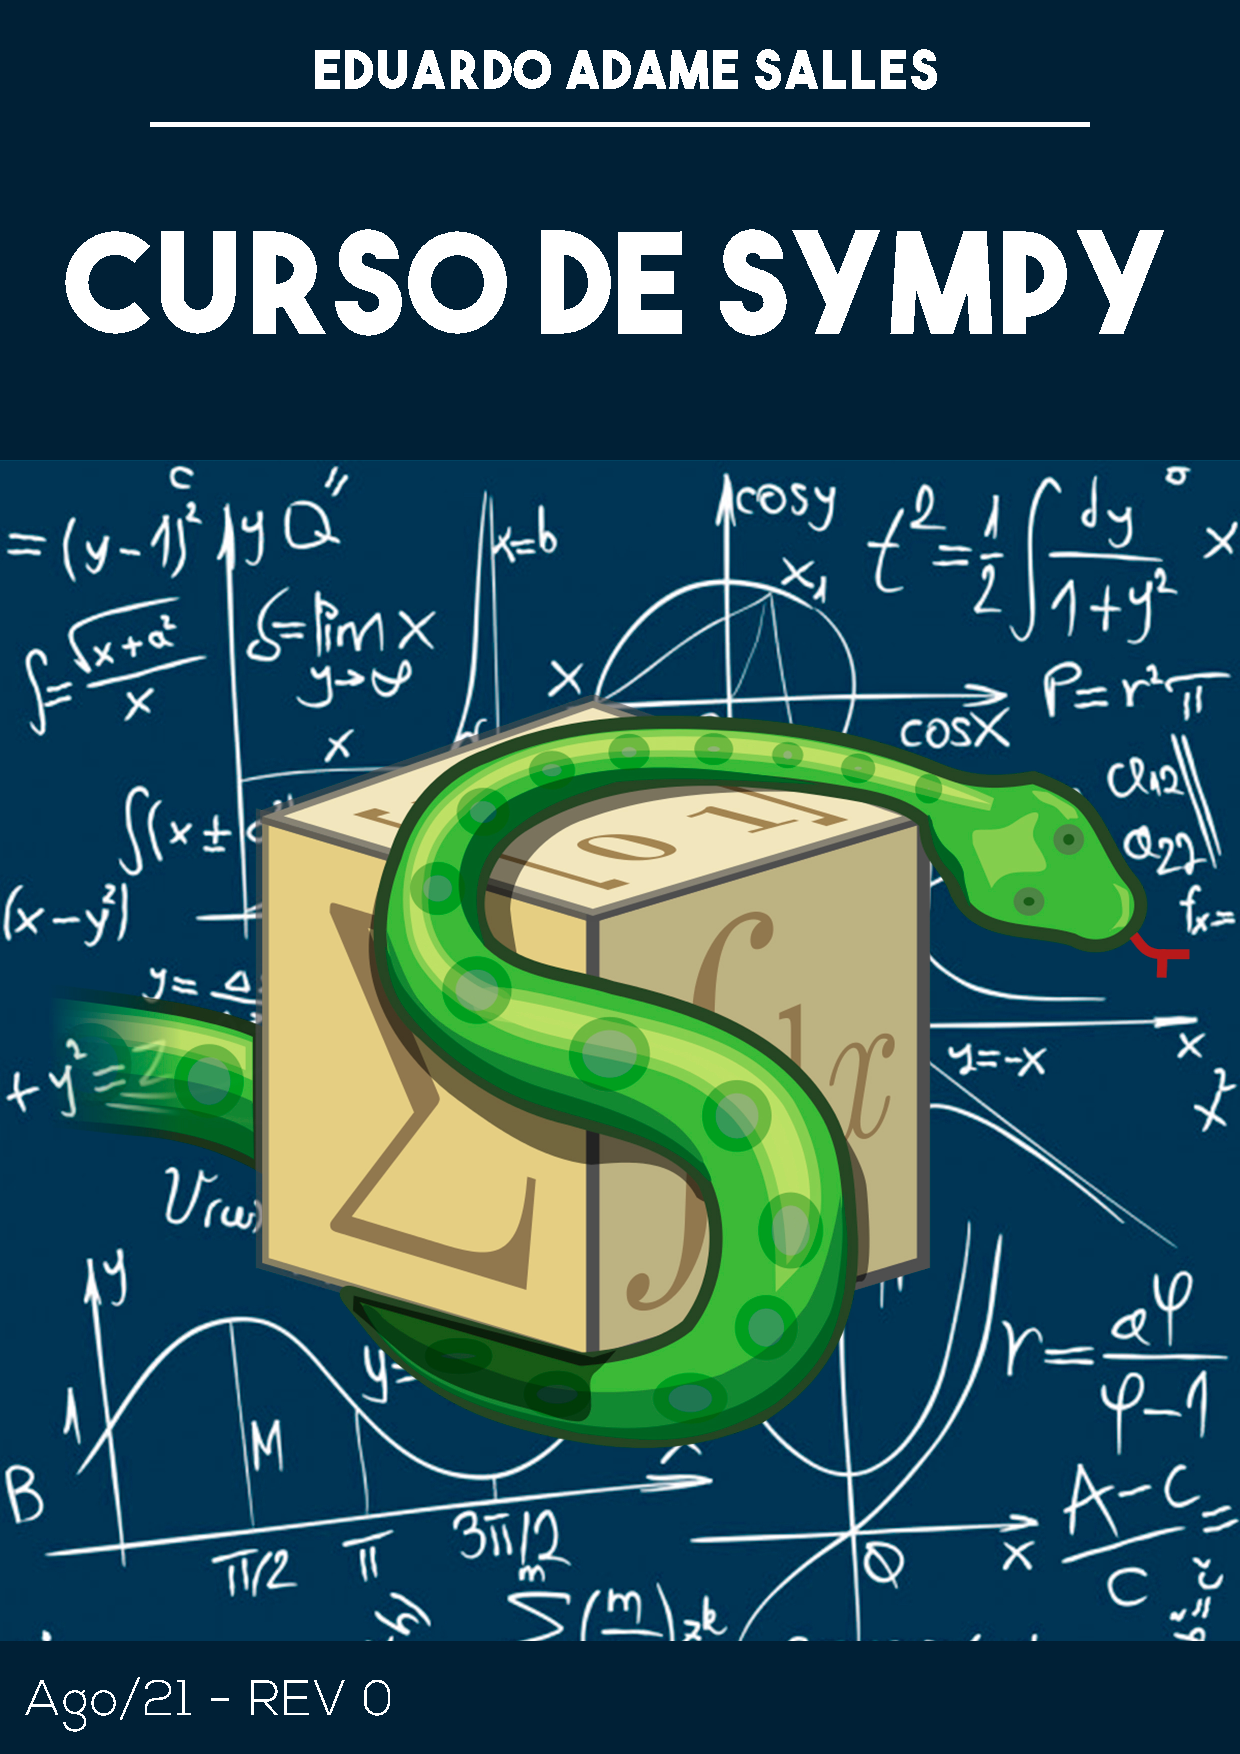
\includepdf{cover.pdf}
    \newpage
    \tableofcontents
    \newpage
    
    \hypertarget{conhecendo-e-preparando-o-ambiente}{%
\section{Conhecendo e Preparando o
Ambiente}\label{conhecendo-e-preparando-o-ambiente}}

\hypertarget{introduuxe7uxe3o}{%
\subsection{Introdução}\label{introduuxe7uxe3o}}

Esse curso busca capacitar seus estudantes no tocante à biblioteca
Sympy, do Python. Portanto, há a necessidade do conhecimento do próprio
Python base. Com isso, o curso foi dividido em uma ordem lógica de
aprendizagem para que o aluno consiga aprender continuamente, sem
grandes ``degraus'' entre os assuntos. O capítulo 1 é uma introdução ao
Python base, o que é suficiente para esse curso.

Neste capítulo, temos como objetivo fazer a instalação e configuração do
nosso ambiente de desenvolvimento. Se você já é desenvolvedor Python,
não acredito que seja necessária sua mudança ao ambiente que será
indicado a esse curso. Mas, caso seja iniciante, recomendo que siga as
instruções.

\hypertarget{escolhendo-um-ambiente}{%
\subsection{Escolhendo um Ambiente}\label{escolhendo-um-ambiente}}

Há duas opções para seguir esse curso:

\begin{enumerate}
\def\labelenumi{\arabic{enumi}.}
\tightlist
\item
  Na forma de Notebooks
\item
  Na forma de Scripts
\end{enumerate}

No curso, serão utilizado notebooks. Mais especificamente, Jupyter
Notebooks, através do ambiente JupyterHub. Mas, não se preocupe, ambas
as opções serão eficientes. Embora a utilização do Sympy seja
regularmente associada ao desenvolvimento em Jupyter.

Na primeira opção, você só terá que instalar um pacote que virá com tudo
incluso (IDE, Pacotes, etc.), e sua programação será mais parecida como
um caderno. Onde você pode escrever, colocar imagens, matemática, e
separar o código em blocos. Contudo, ele é mais pesado e menos flexível.

Na segunda opção, você terá um ambiente mais semelhante à programação
tradicional. Linha após linha e comentários. Você terá que instalar o
Python puro, versionar/atualizar seus módulos manualmente (o que é mais
trabalhoso, mas dá mais autonomia) e utilizar um Editor de Código/IDE.

Caso não tenha entendido o que fora explicado acima, acredito que, nesse
momento inicial, a primeira opção é a melhor para você. Contudo, ela não
te ajudará a migrar para outra linguagem de programação no futuro, caso
queira ou seja necessário. (Isso não é um problema, ao meu ver).

\hypertarget{instalando-o-ambiente-1uxaa-opuxe7uxe3o}{%
\subsection{Instalando o Ambiente (1ª
Opção)}\label{instalando-o-ambiente-1uxaa-opuxe7uxe3o}}

\hypertarget{windows}{%
\subsubsection{Windows}\label{windows}}

No Windows, a instalação é bem simples, utilizaremos o Anaconda. Para
isso, baixe o
\href{https://www.anaconda.com/download/\#windows}{instalador do
Anaconda}.

Prossiga a instalação normalmente. Contudo, preste atenção às duas
caixas de marcação (checkboxes) que perguntam sobre adicionar o Anaconda
ao PATH e torná-lo padrão. Ambas as opções devem estar marcadas.

Se ele oferecer a instalação de algum outro IDE (como o PyCharm), você
pode negar.

\hypertarget{linux}{%
\subsubsection{Linux}\label{linux}}

A instalação no Linux é um pouco mais complicada. Mas, se você utiliza
Linux, possivelmente consegue instalar com certa facilidade.

Verifique as dependências da sua distribuição nesse link:
\url{https://docs.anaconda.com/anaconda/install/linux/}

E depois siga a instalação com o
\href{https://www.anaconda.com/download/\#linux}{instalador para Linux}.
Ele é um instalador em Bash, então recomendo que utilize os comandos
prescritos no site do Anaconda.

\hypertarget{instalando-o-ambiente-2uxaa-opuxe7uxe3o}{%
\subsection{Instalando o Ambiente (2ª
Opção)}\label{instalando-o-ambiente-2uxaa-opuxe7uxe3o}}

Como dito na seção anterior, para essa opção temos que instalar 2
programas, além dos pacotes separadamente.

\hypertarget{windows-1}{%
\subsubsection{Windows}\label{windows-1}}

No Windows, você terá que baixar e instalar o Python que está disponível
nesse link: \url{https://www.python.org/downloads/}

A instalação é bem simples, você só deve se certificar que ele será
adicionado ao PATH e que o \texttt{pip} será instalado. (São duas
caixinhas de marcar que devem aparecer)

Para testar se a instalação deu certo, abra um prompt de comando (basta
inserir ou cmd ou powershell no menu de pesquisa) e digite:

\begin{Shaded}
\begin{Highlighting}[]
\ExtensionTok{py} \AttributeTok{{-}{-}version}
\end{Highlighting}
\end{Shaded}

Deve aparecer a versão do Python que você instalou. Caso isso não
ocorra, repita o procedimento e veja se fez tudo corretamente.

Também confirme se o pip foi instalado corretamente:

\begin{Shaded}
\begin{Highlighting}[]
\ExtensionTok{pip} \AttributeTok{{-}{-}version}
\end{Highlighting}
\end{Shaded}

Após isso, você deve escolher um editor. A minha recomendação é o
\href{https://code.visualstudio.com/}{Visual Studio Code}.

Mas você pode utilizar outros como o \href{https://atom.io/}{Atom} ou
\href{https://www.jetbrains.com/pt-br/pycharm/download/}{PyCharm}.

A instalação de todos é bem simples. Ao abri-los, certifique-se se é
necessário instalar uma extensão para suporte ao Python. Caso for,
instale-a.

\hypertarget{linux-1}{%
\subsubsection{Linux}\label{linux-1}}

No Linux, a imensa maioria das distribuições já vêm com o Python
instalado e disponível. A única diferença é que algumas adotam o nome
\texttt{python3} e outras somente \texttt{python}.

Para isso, teste no terminal:

\begin{Shaded}
\begin{Highlighting}[]
\ExtensionTok{python} \AttributeTok{{-}{-}version}
\ExtensionTok{python3} \AttributeTok{{-}{-}version}
\end{Highlighting}
\end{Shaded}

E comece a usar o que tem a versão mais atual.

Também certifique-se se você tem o \texttt{pip} instalado

\begin{Shaded}
\begin{Highlighting}[]
\ExtensionTok{pip} \AttributeTok{{-}{-}version}
\ExtensionTok{pip3} \AttributeTok{{-}{-}version}
\end{Highlighting}
\end{Shaded}

Caso não tenha, veja como instalá-lo em sua distribuição.

Assim como no Windows, você deve instalar um editor. As minhas
recomendações são as mesmas para o Windows. Ou seja, primeiramente o
\href{https://code.visualstudio.com/}{Visual Studio Code}. E depois ou o
\href{https://atom.io/}{Atom} ou o
\href{https://www.jetbrains.com/pt-br/pycharm/download/}{PyCharm}.

Todos têm versão para Linux e a instalação deve ser até mais simples que
para windows. No caso do Visual Studio Code, recomendo que utilize a
versão flatpak ou snap.

\hypertarget{como-acompanhar-as-explicauxe7uxf5es-do-curso}{%
\subsection{Como acompanhar as explicações do
curso}\label{como-acompanhar-as-explicauxe7uxf5es-do-curso}}

O nosso curso será baseado em Jupyter Notebooks, uma forma de programar
em blocos. Esses blocos podem ser tanto de código como de texto.

No caso, a primeira opção de ambiente lhe entregará um ambiente muito
parecido com o que eu utilizei para escrever os meus Notebooks. Para a
segunda, acredito que será mais difícil. Principalmente, pela ausência
de alguns pacotes e softwares que vêm com o Anaconda. Mas, decidi
incluí-la, pois há pessoas que precisam somente de uma consulta rápida,
e possivelmente já têm seu ambiente de desenvolvimento, sendo em
Anaconda ou não.

Então, para a primeira opção, você deverá abrir o ``Anaconda
Navigator''. Esse software servirá como gerenciador de pacotes e dos
serviços.

Como dito anteriormente, utilizaremos Jupyter Notebooks. Então basta
clicar em ``Launch'' no card do Jupyter Notebook.

Ele abrirá um navegador de arquivos no navegador, semelhante a um site.
Basta escolher uma pasta onde gostaria de criar seus notebooks, e
criá-los a partir do botão ``New'' e então escolha o \emph{Python 3}.

O curso não tem como foco específico ensinar o uso desse ambiente, uma
vez que ele é bem simples. Basicamente, você deverá criar blocos (que
costumamos chamar de \emph{chunks}) de forma a organizar o entendimento
e a saída do seu código. Ao escolher a opção ``Code'' para seu bloco,
você deverá escrever códigos Python nele. No caso de ``Markdown'', você
deverá escrever texto de acordo com a sintaxe da linguagem de marcação
Markdown.

Essa sintaxe é bem simples, dê uma olhada nessa ``tabela de cola'':
\url{https://github.com/luong-komorebi/Markdown-Tutorial/blob/master/README_pt-BR.md}

Para qualquer tipo de bloco, basta segurar a tecla Ctrl e apertar Enter
para compilá-lo.

    \hypertarget{exercuxedcios}{%
\subsection{Exercícios}\label{exercuxedcios}}

\begin{enumerate}
\def\labelenumi{\arabic{enumi}.}
\tightlist
\item
  Crie um chunk de markdown e escreva um título com o texto ``Olá mundo
  em Python''.
\item
  Abaixo desse chunk, crie outro com o código
  \texttt{print(\textquotesingle{}Olá\ mundo\textquotesingle{})}.
\end{enumerate}

    \hypertarget{pruxf3ximos-passos}{%
\subsection{Próximos passos}\label{pruxf3ximos-passos}}

Embora esse capítulo não tenha tido um bloco sequer de código, acredito
que agora estão preparados para aprender os básicos de Python

    \hypertarget{buxe1sicos-da-programauxe7uxe3o-em-python}{%
\section{Básicos da Programação em
Python}\label{buxe1sicos-da-programauxe7uxe3o-em-python}}

\hypertarget{sobre-o-python}{%
\subsection{Sobre o Python}\label{sobre-o-python}}

Não é por acaso que a linguagem de programação Python tem se tornado
cada vez mais popular. Além do seu uso na computação, que ganhou um novo
\emph{hype} por conta da Inteligência Artificial, a linguagem é uma
ótima forma de introduzir uma pessoa à programação, de modo geral.

A linguagem apresenta diversas facilidades em sua sintaxe, que não
somente contibuem para a facilidade da escrita, mas também contribuem
para o entendimento e documentação do código.

Novamente, para não fugir do escopo do curso, não acredito que seja
necessário listar as especificações técnicas da linguagem. Acredito que
há somente alguns conceitos simples que são necessários para o uso da
linguagem.

\begin{itemize}
\tightlist
\item
  O Python é uma linguagem interpretada.
\end{itemize}

Ou seja, o software gerado pelo código é o próprio código interpretado
durante a execução

\begin{itemize}
\tightlist
\item
  O Python interpretará linha após linha, do início ao fim do script
  (chunk, para nós).
\end{itemize}

Para novatos em programação, isso deve ser fácil de aceitar. Mas pessoas
com certa experiência podem questionar essa afirmação. Nesse caso, estou
me referindo a forma que vamos utilizar a linguagem no curso e até onde
iremos com as estruturas de programação da linguagem.

\begin{itemize}
\tightlist
\item
  O Python diferencia letras maíusculas de minúsculas.
\end{itemize}

Isso é chamado de ``sensitive case''. Tome cuidado ao reproduzir os
exemplos e ao programar, de modo geral.

\begin{itemize}
\tightlist
\item
  O Python reconhece espaços vazios.
\end{itemize}

Isso é utilizado para definir o escopo dessa linha de código. Não se
preocupe caso não tenha entendido, é mais simples do que aparenta ser.
Isso basicamente é pra mostrar o ``quão dentro'' uma linha está de uma
estrutura. Abordaremos isso mais tarde.

\begin{itemize}
\tightlist
\item
  Texto precedido por \texttt{\#} não são interpretadas
\end{itemize}

Tudo que vier após um \texttt{\#} em uma linha é chamado de comentário.
Ele não é compilado e utilizaremos para comentar o código.

\hypertarget{definindo-variuxe1veis}{%
\subsection{Definindo variáveis}\label{definindo-variuxe1veis}}

Uma variável é uma forma de armazenar certo valor e reutilizá-lo. Se
quiser fazer uma comparação com a Matemática, apenas enxergue ele como
um \(x_0\) não um \(x\) somente. Ou seja, ele vai ter um valor
específico que pode mudar. Não necessáriamente ele seria ``todos os
valores ao mesmo tempo'' como uma variável na matemática.

Por exemplo, vamos criar a variável \texttt{name} que vai armazenar meu
nome.

    \begin{tcolorbox}[breakable, size=fbox, boxrule=1pt, pad at break*=1mm,colback=cellbackground, colframe=cellborder]
\prompt{In}{incolor}{1}{\boxspacing}
\begin{Verbatim}[commandchars=\\\{\}]
\PY{n}{name} \PY{o}{=} \PY{l+s+s2}{\PYZdq{}}\PY{l+s+s2}{Eduardo}\PY{l+s+s2}{\PYZdq{}}
\end{Verbatim}
\end{tcolorbox}

    Agora, eu posso utilizar name em qualquer lugar do meu código. No caso,
se eu mudar o valor de name, todo lugar onde name está terá seu valor
trocado.

Por exemplo:

    \begin{tcolorbox}[breakable, size=fbox, boxrule=1pt, pad at break*=1mm,colback=cellbackground, colframe=cellborder]
\prompt{In}{incolor}{2}{\boxspacing}
\begin{Verbatim}[commandchars=\\\{\}]
\PY{n}{name} \PY{o}{=} \PY{l+s+s2}{\PYZdq{}}\PY{l+s+s2}{Eduardo}\PY{l+s+s2}{\PYZdq{}}
\PY{n}{name}
\end{Verbatim}
\end{tcolorbox}

            \begin{tcolorbox}[breakable, size=fbox, boxrule=.5pt, pad at break*=1mm, opacityfill=0]
\prompt{Out}{outcolor}{2}{\boxspacing}
\begin{Verbatim}[commandchars=\\\{\}]
'Eduardo'
\end{Verbatim}
\end{tcolorbox}
        
    \begin{tcolorbox}[breakable, size=fbox, boxrule=1pt, pad at break*=1mm,colback=cellbackground, colframe=cellborder]
\prompt{In}{incolor}{3}{\boxspacing}
\begin{Verbatim}[commandchars=\\\{\}]
\PY{n}{name} \PY{o}{=} \PY{l+s+s2}{\PYZdq{}}\PY{l+s+s2}{Adame}\PY{l+s+s2}{\PYZdq{}}
\PY{n}{name}
\end{Verbatim}
\end{tcolorbox}

            \begin{tcolorbox}[breakable, size=fbox, boxrule=.5pt, pad at break*=1mm, opacityfill=0]
\prompt{Out}{outcolor}{3}{\boxspacing}
\begin{Verbatim}[commandchars=\\\{\}]
'Adame'
\end{Verbatim}
\end{tcolorbox}
        
    Para ficar mais claro, podemos ver algo como:

    \begin{tcolorbox}[breakable, size=fbox, boxrule=1pt, pad at break*=1mm,colback=cellbackground, colframe=cellborder]
\prompt{In}{incolor}{4}{\boxspacing}
\begin{Verbatim}[commandchars=\\\{\}]
\PY{n}{name} \PY{o}{=} \PY{l+s+s2}{\PYZdq{}}\PY{l+s+s2}{Eduardo}\PY{l+s+s2}{\PYZdq{}}
\PY{n}{name} \PY{o}{=} \PY{l+s+s2}{\PYZdq{}}\PY{l+s+s2}{Adame}\PY{l+s+s2}{\PYZdq{}}
\PY{n}{name}
\end{Verbatim}
\end{tcolorbox}

            \begin{tcolorbox}[breakable, size=fbox, boxrule=.5pt, pad at break*=1mm, opacityfill=0]
\prompt{Out}{outcolor}{4}{\boxspacing}
\begin{Verbatim}[commandchars=\\\{\}]
'Adame'
\end{Verbatim}
\end{tcolorbox}
        
    Como pôde ver no \emph{chunk} acima, embora eu tenha atribuído o valor
\texttt{"Eduardo"} ao \texttt{name} na primeira linha, o valor dele foi
sobrescrito pela linha seguinte.

\hypertarget{tipos-de-variuxe1veis}{%
\subsection{Tipos de Variáveis}\label{tipos-de-variuxe1veis}}

Acredito que deve ter notado que colocamos o valor entre \texttt{"\ "}.
Por quê?

Isso tem a ver com o tipo do valor. No Python, os tipos são
dinamicamente interpretados através de sua sintaxe. E, nesse caso, nós
inserimos uma \texttt{string}, que é utilizada para armazenar texto.

Vamos falar sobre os principais tipos de variáveis que já vêm com o
Python e como defini-las.

\hypertarget{inteiros}{%
\subsubsection{Inteiros}\label{inteiros}}

Os inteiros são simplesmente definidos ao igualar uma variável a um
número que pertença ao conjunto dos números inteiros, seja positivo ou
negativo.

    \begin{tcolorbox}[breakable, size=fbox, boxrule=1pt, pad at break*=1mm,colback=cellbackground, colframe=cellborder]
\prompt{In}{incolor}{5}{\boxspacing}
\begin{Verbatim}[commandchars=\\\{\}]
\PY{n}{my\PYZus{}integer} \PY{o}{=} \PY{l+m+mi}{2}
\PY{n}{my\PYZus{}integer}
\end{Verbatim}
\end{tcolorbox}

            \begin{tcolorbox}[breakable, size=fbox, boxrule=.5pt, pad at break*=1mm, opacityfill=0]
\prompt{Out}{outcolor}{5}{\boxspacing}
\begin{Verbatim}[commandchars=\\\{\}]
2
\end{Verbatim}
\end{tcolorbox}
        
    \hypertarget{floats}{%
\subsubsection{Floats}\label{floats}}

Os floats, diferentemente dos inteiros, podem ser qualquer número real.
Utilizamos ponto (\texttt{.}) para separar as casas decimais.

    \begin{tcolorbox}[breakable, size=fbox, boxrule=1pt, pad at break*=1mm,colback=cellbackground, colframe=cellborder]
\prompt{In}{incolor}{6}{\boxspacing}
\begin{Verbatim}[commandchars=\\\{\}]
\PY{n}{my\PYZus{}float} \PY{o}{=} \PY{l+m+mf}{2.5}
\PY{n}{my\PYZus{}float}
\end{Verbatim}
\end{tcolorbox}

            \begin{tcolorbox}[breakable, size=fbox, boxrule=.5pt, pad at break*=1mm, opacityfill=0]
\prompt{Out}{outcolor}{6}{\boxspacing}
\begin{Verbatim}[commandchars=\\\{\}]
2.5
\end{Verbatim}
\end{tcolorbox}
        
    \hypertarget{strings}{%
\subsubsection{Strings}\label{strings}}

Como dito anteriormente, strings são utilizados para textos. Basta
envolver seu texto em aspas (\texttt{"\ "}) ou
(\texttt{\textquotesingle{}\ \textquotesingle{}}). Para o Python, tanto
faz se elas são simples ou duplas.

    \begin{tcolorbox}[breakable, size=fbox, boxrule=1pt, pad at break*=1mm,colback=cellbackground, colframe=cellborder]
\prompt{In}{incolor}{7}{\boxspacing}
\begin{Verbatim}[commandchars=\\\{\}]
\PY{n}{my\PYZus{}string} \PY{o}{=} \PY{l+s+s2}{\PYZdq{}}\PY{l+s+s2}{Textos são bem úteis, não acha?}\PY{l+s+s2}{\PYZdq{}}
\PY{n}{my\PYZus{}string}
\end{Verbatim}
\end{tcolorbox}

            \begin{tcolorbox}[breakable, size=fbox, boxrule=.5pt, pad at break*=1mm, opacityfill=0]
\prompt{Out}{outcolor}{7}{\boxspacing}
\begin{Verbatim}[commandchars=\\\{\}]
'Textos são bem úteis, não acha?'
\end{Verbatim}
\end{tcolorbox}
        
    \hypertarget{booleanos}{%
\subsubsection{Booleanos}\label{booleanos}}

Esse tipo de valor é utilizado para condições. Eles podem ser ``Falso''
(\texttt{False}) ou ``Verdadeiro'' (\texttt{True}). Preste atenção no
sensitive case.

    \begin{tcolorbox}[breakable, size=fbox, boxrule=1pt, pad at break*=1mm,colback=cellbackground, colframe=cellborder]
\prompt{In}{incolor}{8}{\boxspacing}
\begin{Verbatim}[commandchars=\\\{\}]
\PY{n}{do\PYZus{}i\PYZus{}like\PYZus{}math} \PY{o}{=} \PY{k+kc}{True}
\PY{n}{do\PYZus{}i\PYZus{}like\PYZus{}rlang} \PY{o}{=} \PY{k+kc}{False}
\PY{n}{do\PYZus{}i\PYZus{}like\PYZus{}math}\PY{p}{,} \PY{n}{do\PYZus{}i\PYZus{}like\PYZus{}rlang}
\end{Verbatim}
\end{tcolorbox}

            \begin{tcolorbox}[breakable, size=fbox, boxrule=.5pt, pad at break*=1mm, opacityfill=0]
\prompt{Out}{outcolor}{8}{\boxspacing}
\begin{Verbatim}[commandchars=\\\{\}]
(True, False)
\end{Verbatim}
\end{tcolorbox}
        
    \hypertarget{listas}{%
\subsubsection{Listas}\label{listas}}

Nós utilizamos listas para agrupar outros valores. Uma lista pode
armazenar qualquer tipo e em qualquer quantidade. Inclusive podemos
fazer listas de listas.

    \begin{tcolorbox}[breakable, size=fbox, boxrule=1pt, pad at break*=1mm,colback=cellbackground, colframe=cellborder]
\prompt{In}{incolor}{9}{\boxspacing}
\begin{Verbatim}[commandchars=\\\{\}]
\PY{n}{names} \PY{o}{=} \PY{p}{[}\PY{l+s+s2}{\PYZdq{}}\PY{l+s+s2}{Eduardo}\PY{l+s+s2}{\PYZdq{}}\PY{p}{,} \PY{l+s+s2}{\PYZdq{}}\PY{l+s+s2}{Marcos}\PY{l+s+s2}{\PYZdq{}}\PY{p}{,} \PY{l+s+s2}{\PYZdq{}}\PY{l+s+s2}{Ruan}\PY{l+s+s2}{\PYZdq{}}\PY{p}{,} \PY{l+s+s2}{\PYZdq{}}\PY{l+s+s2}{João}\PY{l+s+s2}{\PYZdq{}}\PY{p}{]}
\PY{n}{names}
\end{Verbatim}
\end{tcolorbox}

            \begin{tcolorbox}[breakable, size=fbox, boxrule=.5pt, pad at break*=1mm, opacityfill=0]
\prompt{Out}{outcolor}{9}{\boxspacing}
\begin{Verbatim}[commandchars=\\\{\}]
['Eduardo', 'Marcos', 'Ruan', 'João']
\end{Verbatim}
\end{tcolorbox}
        
    \begin{tcolorbox}[breakable, size=fbox, boxrule=1pt, pad at break*=1mm,colback=cellbackground, colframe=cellborder]
\prompt{In}{incolor}{10}{\boxspacing}
\begin{Verbatim}[commandchars=\\\{\}]
\PY{n}{my\PYZus{}id} \PY{o}{=} \PY{p}{[}\PY{l+s+s2}{\PYZdq{}}\PY{l+s+s2}{Eduardo}\PY{l+s+s2}{\PYZdq{}}\PY{p}{,} \PY{l+m+mi}{18}\PY{p}{,} \PY{l+m+mf}{1.78}\PY{p}{]}
\PY{n}{my\PYZus{}id}
\end{Verbatim}
\end{tcolorbox}

            \begin{tcolorbox}[breakable, size=fbox, boxrule=.5pt, pad at break*=1mm, opacityfill=0]
\prompt{Out}{outcolor}{10}{\boxspacing}
\begin{Verbatim}[commandchars=\\\{\}]
['Eduardo', 18, 1.78]
\end{Verbatim}
\end{tcolorbox}
        
    Para acessar um valor em específico na lista utilizamos \texttt{{[}{]}}
com o índice desse valor. A lista começa a contagem em 0. Veremos
algumas outras coisas necessárias para o uso de listas posteriormente.

    \begin{tcolorbox}[breakable, size=fbox, boxrule=1pt, pad at break*=1mm,colback=cellbackground, colframe=cellborder]
\prompt{In}{incolor}{11}{\boxspacing}
\begin{Verbatim}[commandchars=\\\{\}]
\PY{n}{names}\PY{p}{[}\PY{l+m+mi}{1}\PY{p}{]} \PY{c+c1}{\PYZsh{} \PYZdq{}Eduardo\PYZdq{} é o 0}
\end{Verbatim}
\end{tcolorbox}

            \begin{tcolorbox}[breakable, size=fbox, boxrule=.5pt, pad at break*=1mm, opacityfill=0]
\prompt{Out}{outcolor}{11}{\boxspacing}
\begin{Verbatim}[commandchars=\\\{\}]
'Marcos'
\end{Verbatim}
\end{tcolorbox}
        
    \begin{tcolorbox}[breakable, size=fbox, boxrule=1pt, pad at break*=1mm,colback=cellbackground, colframe=cellborder]
\prompt{In}{incolor}{12}{\boxspacing}
\begin{Verbatim}[commandchars=\\\{\}]
\PY{n}{my\PYZus{}id}\PY{p}{[}\PY{l+m+mi}{2}\PY{p}{]}
\end{Verbatim}
\end{tcolorbox}

            \begin{tcolorbox}[breakable, size=fbox, boxrule=.5pt, pad at break*=1mm, opacityfill=0]
\prompt{Out}{outcolor}{12}{\boxspacing}
\begin{Verbatim}[commandchars=\\\{\}]
1.78
\end{Verbatim}
\end{tcolorbox}
        
    \hypertarget{operauxe7uxf5es}{%
\subsection{Operações}\label{operauxe7uxf5es}}

Os operadores e as operações para cada tipo são diferentes.
Principalmente quando ocorrem entre dois tipos diferentes. Os principais
para cada um deles são:

\hypertarget{aritmuxe9tica} para módulo (resto).
\end{itemize}

Para alguns exemplos, como esse, não criarei variáveis, mas é possível
criar para qualquer operação.

    \begin{tcolorbox}[breakable, size=fbox, boxrule=1pt, pad at break*=1mm,colback=cellbackground, colframe=cellborder]
\prompt{In}{incolor}{13}{\boxspacing}
\begin{Verbatim}[commandchars=\\\{\}]
\PY{l+m+mi}{5} \PY{o}{+} \PY{l+m+mi}{2} \PY{o}{+} \PY{l+m+mi}{4} \PY{o}{*} \PY{l+m+mi}{10} 
\end{Verbatim}
\end{tcolorbox}

            \begin{tcolorbox}[breakable, size=fbox, boxrule=.5pt, pad at break*=1mm, opacityfill=0]
\prompt{Out}{outcolor}{13}{\boxspacing}
\begin{Verbatim}[commandchars=\\\{\}]
47
\end{Verbatim}
\end{tcolorbox}
        
    \begin{tcolorbox}[breakable, size=fbox, boxrule=1pt, pad at break*=1mm,colback=cellbackground, colframe=cellborder]
\prompt{In}{incolor}{14}{\boxspacing}
\begin{Verbatim}[commandchars=\\\{\}]
\PY{l+m+mi}{2} \PY{o}{*}\PY{o}{*} \PY{p}{(}\PY{l+m+mi}{1}\PY{o}{/}\PY{l+m+mi}{2}\PY{p}{)} \PY{c+c1}{\PYZsh{} Raíz de 2}
\end{Verbatim}
\end{tcolorbox}

            \begin{tcolorbox}[breakable, size=fbox, boxrule=.5pt, pad at break*=1mm, opacityfill=0]
\prompt{Out}{outcolor}{14}{\boxspacing}
\begin{Verbatim}[commandchars=\\\{\}]
1.4142135623730951
\end{Verbatim}
\end{tcolorbox}
        
    Você também pode utilizar esses operadores em cima de uma variável. Por
exemplo, você tem uma variável e quer acrescer 2 nela.

    \begin{tcolorbox}[breakable, size=fbox, boxrule=1pt, pad at break*=1mm,colback=cellbackground, colframe=cellborder]
\prompt{In}{incolor}{15}{\boxspacing}
\begin{Verbatim}[commandchars=\\\{\}]
\PY{n}{my\PYZus{}num} \PY{o}{=} \PY{l+m+mi}{14}
\PY{n}{my\PYZus{}num} \PY{o}{=} \PY{n}{my\PYZus{}num} \PY{o}{+} \PY{l+m+mi}{2}
\PY{n}{my\PYZus{}num}
\end{Verbatim}
\end{tcolorbox}

            \begin{tcolorbox}[breakable, size=fbox, boxrule=.5pt, pad at break*=1mm, opacityfill=0]
\prompt{Out}{outcolor}{15}{\boxspacing}
\begin{Verbatim}[commandchars=\\\{\}]
16
\end{Verbatim}
\end{tcolorbox}
        
    O exemplo acima é bem convincente e, certamente, bem útil. Mas há uma
forma reduzida desse tipo de expressão.

    \begin{tcolorbox}[breakable, size=fbox, boxrule=1pt, pad at break*=1mm,colback=cellbackground, colframe=cellborder]
\prompt{In}{incolor}{16}{\boxspacing}
\begin{Verbatim}[commandchars=\\\{\}]
\PY{n}{my\PYZus{}num} \PY{o}{=} \PY{l+m+mi}{14}
\PY{n}{my\PYZus{}num} \PY{o}{+}\PY{o}{=} \PY{l+m+mi}{2}
\PY{n}{my\PYZus{}num}
\end{Verbatim}
\end{tcolorbox}

            \begin{tcolorbox}[breakable, size=fbox, boxrule=.5pt, pad at break*=1mm, opacityfill=0]
\prompt{Out}{outcolor}{16}{\boxspacing}
\begin{Verbatim}[commandchars=\\\{\}]
16
\end{Verbatim}
\end{tcolorbox}
        
    Esse tipo de ``operador'' pode ser criado ao unir um desses operadores
listados acima com o símbolo de \texttt{=}.

    \begin{tcolorbox}[breakable, size=fbox, boxrule=1pt, pad at break*=1mm,colback=cellbackground, colframe=cellborder]
\prompt{In}{incolor}{17}{\boxspacing}
\begin{Verbatim}[commandchars=\\\{\}]
\PY{n}{my\PYZus{}num} \PY{o}{=} \PY{l+m+mi}{2}
\PY{n}{my\PYZus{}num} \PY{o}{*}\PY{o}{=} \PY{l+m+mi}{10}
\PY{n}{my\PYZus{}num}
\end{Verbatim}
\end{tcolorbox}

            \begin{tcolorbox}[breakable, size=fbox, boxrule=.5pt, pad at break*=1mm, opacityfill=0]
\prompt{Out}{outcolor}{17}{\boxspacing}
\begin{Verbatim}[commandchars=\\\{\}]
20
\end{Verbatim}
\end{tcolorbox}
        
    \hypertarget{booleanas}{%
\subsubsection{Booleanas}\label{booleanas}}

As operações booleanas são expressões que retornam ou \texttt{True} ou
\texttt{False}, são utilizadas para condições.

No Python, costumamos escrever por extenso a maioria das condições.

\begin{itemize}
\tightlist
\item
  \texttt{and} para operação ``e''
\item
  \texttt{or} para operação ``ou''
\item
  \texttt{not} para operação de negação (inverte o valor)
\item
  \texttt{\textgreater{}}/\texttt{\textgreater{}=} maior/maior ou igual
\item
  \texttt{\textless{}}/\texttt{\textless{}=} menor/menor ou igual
\item
  \texttt{==} igual
\item
  \texttt{in}confere está em uma lista
\end{itemize}

Exemplos:

    \begin{tcolorbox}[breakable, size=fbox, boxrule=1pt, pad at break*=1mm,colback=cellbackground, colframe=cellborder]
\prompt{In}{incolor}{18}{\boxspacing}
\begin{Verbatim}[commandchars=\\\{\}]
\PY{l+m+mi}{30} \PY{o}{\PYZgt{}} \PY{l+m+mi}{15}
\end{Verbatim}
\end{tcolorbox}

            \begin{tcolorbox}[breakable, size=fbox, boxrule=.5pt, pad at break*=1mm, opacityfill=0]
\prompt{Out}{outcolor}{18}{\boxspacing}
\begin{Verbatim}[commandchars=\\\{\}]
True
\end{Verbatim}
\end{tcolorbox}
        
    \begin{tcolorbox}[breakable, size=fbox, boxrule=1pt, pad at break*=1mm,colback=cellbackground, colframe=cellborder]
\prompt{In}{incolor}{19}{\boxspacing}
\begin{Verbatim}[commandchars=\\\{\}]
\PY{l+m+mi}{30} \PY{o}{\PYZlt{}} \PY{l+m+mi}{15}
\end{Verbatim}
\end{tcolorbox}

            \begin{tcolorbox}[breakable, size=fbox, boxrule=.5pt, pad at break*=1mm, opacityfill=0]
\prompt{Out}{outcolor}{19}{\boxspacing}
\begin{Verbatim}[commandchars=\\\{\}]
False
\end{Verbatim}
\end{tcolorbox}
        
    \begin{tcolorbox}[breakable, size=fbox, boxrule=1pt, pad at break*=1mm,colback=cellbackground, colframe=cellborder]
\prompt{In}{incolor}{20}{\boxspacing}
\begin{Verbatim}[commandchars=\\\{\}]
\PY{l+m+mi}{14} \PY{o}{==} \PY{l+m+mi}{14}
\end{Verbatim}
\end{tcolorbox}

            \begin{tcolorbox}[breakable, size=fbox, boxrule=.5pt, pad at break*=1mm, opacityfill=0]
\prompt{Out}{outcolor}{20}{\boxspacing}
\begin{Verbatim}[commandchars=\\\{\}]
True
\end{Verbatim}
\end{tcolorbox}
        
    \begin{tcolorbox}[breakable, size=fbox, boxrule=1pt, pad at break*=1mm,colback=cellbackground, colframe=cellborder]
\prompt{In}{incolor}{21}{\boxspacing}
\begin{Verbatim}[commandchars=\\\{\}]
\PY{l+m+mi}{30} \PY{o}{\PYZlt{}} \PY{l+m+mi}{15} \PY{o+ow}{and} \PY{l+m+mi}{14} \PY{o}{==} \PY{l+m+mi}{14}
\end{Verbatim}
\end{tcolorbox}

            \begin{tcolorbox}[breakable, size=fbox, boxrule=.5pt, pad at break*=1mm, opacityfill=0]
\prompt{Out}{outcolor}{21}{\boxspacing}
\begin{Verbatim}[commandchars=\\\{\}]
False
\end{Verbatim}
\end{tcolorbox}
        
    \begin{tcolorbox}[breakable, size=fbox, boxrule=1pt, pad at break*=1mm,colback=cellbackground, colframe=cellborder]
\prompt{In}{incolor}{22}{\boxspacing}
\begin{Verbatim}[commandchars=\\\{\}]
\PY{l+m+mi}{30} \PY{o}{\PYZlt{}}\PY{o}{=} \PY{l+m+mi}{15} \PY{o+ow}{or} \PY{l+m+mi}{14} \PY{o}{==} \PY{l+m+mi}{14}
\end{Verbatim}
\end{tcolorbox}

            \begin{tcolorbox}[breakable, size=fbox, boxrule=.5pt, pad at break*=1mm, opacityfill=0]
\prompt{Out}{outcolor}{22}{\boxspacing}
\begin{Verbatim}[commandchars=\\\{\}]
True
\end{Verbatim}
\end{tcolorbox}
        
    \begin{tcolorbox}[breakable, size=fbox, boxrule=1pt, pad at break*=1mm,colback=cellbackground, colframe=cellborder]
\prompt{In}{incolor}{23}{\boxspacing}
\begin{Verbatim}[commandchars=\\\{\}]
\PY{l+m+mi}{14}\PY{o}{==}\PY{l+m+mi}{14} \PY{o+ow}{and} \PY{o+ow}{not} \PY{l+m+mi}{30} \PY{o}{\PYZlt{}} \PY{l+m+mi}{15}
\end{Verbatim}
\end{tcolorbox}

            \begin{tcolorbox}[breakable, size=fbox, boxrule=.5pt, pad at break*=1mm, opacityfill=0]
\prompt{Out}{outcolor}{23}{\boxspacing}
\begin{Verbatim}[commandchars=\\\{\}]
True
\end{Verbatim}
\end{tcolorbox}
        
    \begin{tcolorbox}[breakable, size=fbox, boxrule=1pt, pad at break*=1mm,colback=cellbackground, colframe=cellborder]
\prompt{In}{incolor}{24}{\boxspacing}
\begin{Verbatim}[commandchars=\\\{\}]
\PY{n}{lst} \PY{o}{=} \PY{p}{[}\PY{l+m+mi}{1}\PY{p}{,}\PY{l+m+mi}{2}\PY{p}{]}
\PY{l+m+mi}{2} \PY{o+ow}{in} \PY{n}{lst}
\end{Verbatim}
\end{tcolorbox}

            \begin{tcolorbox}[breakable, size=fbox, boxrule=.5pt, pad at break*=1mm, opacityfill=0]
\prompt{Out}{outcolor}{24}{\boxspacing}
\begin{Verbatim}[commandchars=\\\{\}]
True
\end{Verbatim}
\end{tcolorbox}
        
    \begin{tcolorbox}[breakable, size=fbox, boxrule=1pt, pad at break*=1mm,colback=cellbackground, colframe=cellborder]
\prompt{In}{incolor}{25}{\boxspacing}
\begin{Verbatim}[commandchars=\\\{\}]
\PY{k+kc}{True} \PY{o+ow}{and} \PY{k+kc}{False}
\end{Verbatim}
\end{tcolorbox}

            \begin{tcolorbox}[breakable, size=fbox, boxrule=.5pt, pad at break*=1mm, opacityfill=0]
\prompt{Out}{outcolor}{25}{\boxspacing}
\begin{Verbatim}[commandchars=\\\{\}]
False
\end{Verbatim}
\end{tcolorbox}
        
    \begin{tcolorbox}[breakable, size=fbox, boxrule=1pt, pad at break*=1mm,colback=cellbackground, colframe=cellborder]
\prompt{In}{incolor}{26}{\boxspacing}
\begin{Verbatim}[commandchars=\\\{\}]
\PY{k+kc}{False} \PY{o+ow}{or} \PY{o+ow}{not} \PY{k+kc}{False}
\end{Verbatim}
\end{tcolorbox}

            \begin{tcolorbox}[breakable, size=fbox, boxrule=.5pt, pad at break*=1mm, opacityfill=0]
\prompt{Out}{outcolor}{26}{\boxspacing}
\begin{Verbatim}[commandchars=\\\{\}]
True
\end{Verbatim}
\end{tcolorbox}
        
    \hypertarget{strings}{%
\subsubsection{Strings}\label{strings}}

Podemos formatar strings e fazer algumas operações com elas

\begin{itemize}
\tightlist
\item
  \texttt{+} para concatenação
\item
  \texttt{*} para concatenação repetidas vezes
\end{itemize}

Exemplos:

    \begin{tcolorbox}[breakable, size=fbox, boxrule=1pt, pad at break*=1mm,colback=cellbackground, colframe=cellborder]
\prompt{In}{incolor}{27}{\boxspacing}
\begin{Verbatim}[commandchars=\\\{\}]
\PY{l+s+s1}{\PYZsq{}}\PY{l+s+s1}{Eduardo }\PY{l+s+s1}{\PYZsq{}} \PY{o}{+} \PY{l+s+s1}{\PYZsq{}}\PY{l+s+s1}{Adame}\PY{l+s+s1}{\PYZsq{}}
\end{Verbatim}
\end{tcolorbox}

            \begin{tcolorbox}[breakable, size=fbox, boxrule=.5pt, pad at break*=1mm, opacityfill=0]
\prompt{Out}{outcolor}{27}{\boxspacing}
\begin{Verbatim}[commandchars=\\\{\}]
'Eduardo Adame'
\end{Verbatim}
\end{tcolorbox}
        
    \begin{tcolorbox}[breakable, size=fbox, boxrule=1pt, pad at break*=1mm,colback=cellbackground, colframe=cellborder]
\prompt{In}{incolor}{28}{\boxspacing}
\begin{Verbatim}[commandchars=\\\{\}]
\PY{l+s+s1}{\PYZsq{}}\PY{l+s+s1}{du}\PY{l+s+s1}{\PYZsq{}}\PY{o}{*}\PY{l+m+mi}{2}
\end{Verbatim}
\end{tcolorbox}

            \begin{tcolorbox}[breakable, size=fbox, boxrule=.5pt, pad at break*=1mm, opacityfill=0]
\prompt{Out}{outcolor}{28}{\boxspacing}
\begin{Verbatim}[commandchars=\\\{\}]
'dudu'
\end{Verbatim}
\end{tcolorbox}
        
    \hypertarget{strings-formatadas}{%
\paragraph{Strings formatadas}\label{strings-formatadas}}

As strings formatadas são um modo de inserir variáveis em strings.
Adicionamos um \texttt{f} antes das áspas e colocamos a variável entre
chaves \texttt{\{\}}.

Exemplo:

    \begin{tcolorbox}[breakable, size=fbox, boxrule=1pt, pad at break*=1mm,colback=cellbackground, colframe=cellborder]
\prompt{In}{incolor}{29}{\boxspacing}
\begin{Verbatim}[commandchars=\\\{\}]
\PY{n}{nome} \PY{o}{=} \PY{l+s+s1}{\PYZsq{}}\PY{l+s+s1}{Eduardo}\PY{l+s+s1}{\PYZsq{}}
\PY{n}{sobrenome} \PY{o}{=} \PY{l+s+s1}{\PYZsq{}}\PY{l+s+s1}{Adame}\PY{l+s+s1}{\PYZsq{}}
\PY{n}{idade} \PY{o}{=} \PY{l+m+mi}{18}
\PY{l+s+sa}{f}\PY{l+s+s1}{\PYZsq{}}\PY{l+s+s1}{Meu nome é }\PY{l+s+si}{\PYZob{}}\PY{n}{nome}\PY{l+s+si}{\PYZcb{}}\PY{l+s+s1}{ }\PY{l+s+si}{\PYZob{}}\PY{n}{sobrenome}\PY{l+s+si}{\PYZcb{}}\PY{l+s+s1}{ e tenho }\PY{l+s+si}{\PYZob{}}\PY{n}{idade}\PY{l+s+si}{\PYZcb{}}\PY{l+s+s1}{ anos}\PY{l+s+s1}{\PYZsq{}}
\end{Verbatim}
\end{tcolorbox}

            \begin{tcolorbox}[breakable, size=fbox, boxrule=.5pt, pad at break*=1mm, opacityfill=0]
\prompt{Out}{outcolor}{29}{\boxspacing}
\begin{Verbatim}[commandchars=\\\{\}]
'Meu nome é Eduardo Adame e tenho 18 anos'
\end{Verbatim}
\end{tcolorbox}
        
    \hypertarget{conversuxe3o-de-tipos}{%
\subsection{Conversão de Tipos}\label{conversuxe3o-de-tipos}}

Basta utilizar a função (veremos mais tarde funções em específico) que
tem o nome do tipo.

\begin{itemize}
\tightlist
\item
  \texttt{int()} para converter para \texttt{inteiro}
\item
  \texttt{str()} para converter para \texttt{string}
\item
  \texttt{bool()} para converter para \texttt{booleano}
\item
  \texttt{float()} para converter para \texttt{float}
\end{itemize}

    \begin{tcolorbox}[breakable, size=fbox, boxrule=1pt, pad at break*=1mm,colback=cellbackground, colframe=cellborder]
\prompt{In}{incolor}{30}{\boxspacing}
\begin{Verbatim}[commandchars=\\\{\}]
\PY{n+nb}{int}\PY{p}{(}\PY{l+s+s1}{\PYZsq{}}\PY{l+s+s1}{10}\PY{l+s+s1}{\PYZsq{}}\PY{p}{)}
\end{Verbatim}
\end{tcolorbox}

            \begin{tcolorbox}[breakable, size=fbox, boxrule=.5pt, pad at break*=1mm, opacityfill=0]
\prompt{Out}{outcolor}{30}{\boxspacing}
\begin{Verbatim}[commandchars=\\\{\}]
10
\end{Verbatim}
\end{tcolorbox}
        
    \begin{tcolorbox}[breakable, size=fbox, boxrule=1pt, pad at break*=1mm,colback=cellbackground, colframe=cellborder]
\prompt{In}{incolor}{31}{\boxspacing}
\begin{Verbatim}[commandchars=\\\{\}]
\PY{n+nb}{int}\PY{p}{(}\PY{l+m+mf}{20.0}\PY{p}{)}
\end{Verbatim}
\end{tcolorbox}

            \begin{tcolorbox}[breakable, size=fbox, boxrule=.5pt, pad at break*=1mm, opacityfill=0]
\prompt{Out}{outcolor}{31}{\boxspacing}
\begin{Verbatim}[commandchars=\\\{\}]
20
\end{Verbatim}
\end{tcolorbox}
        
    \begin{tcolorbox}[breakable, size=fbox, boxrule=1pt, pad at break*=1mm,colback=cellbackground, colframe=cellborder]
\prompt{In}{incolor}{32}{\boxspacing}
\begin{Verbatim}[commandchars=\\\{\}]
\PY{n+nb}{float}\PY{p}{(}\PY{l+s+s1}{\PYZsq{}}\PY{l+s+s1}{12.23}\PY{l+s+s1}{\PYZsq{}}\PY{p}{)}
\end{Verbatim}
\end{tcolorbox}

            \begin{tcolorbox}[breakable, size=fbox, boxrule=.5pt, pad at break*=1mm, opacityfill=0]
\prompt{Out}{outcolor}{32}{\boxspacing}
\begin{Verbatim}[commandchars=\\\{\}]
12.23
\end{Verbatim}
\end{tcolorbox}
        
    \begin{tcolorbox}[breakable, size=fbox, boxrule=1pt, pad at break*=1mm,colback=cellbackground, colframe=cellborder]
\prompt{In}{incolor}{33}{\boxspacing}
\begin{Verbatim}[commandchars=\\\{\}]
\PY{n+nb}{str}\PY{p}{(}\PY{l+m+mf}{30.2}\PY{p}{)}
\end{Verbatim}
\end{tcolorbox}

            \begin{tcolorbox}[breakable, size=fbox, boxrule=.5pt, pad at break*=1mm, opacityfill=0]
\prompt{Out}{outcolor}{33}{\boxspacing}
\begin{Verbatim}[commandchars=\\\{\}]
'30.2'
\end{Verbatim}
\end{tcolorbox}
        
    \begin{tcolorbox}[breakable, size=fbox, boxrule=1pt, pad at break*=1mm,colback=cellbackground, colframe=cellborder]
\prompt{In}{incolor}{34}{\boxspacing}
\begin{Verbatim}[commandchars=\\\{\}]
\PY{n+nb}{bool}\PY{p}{(}\PY{l+m+mi}{0}\PY{p}{)}
\end{Verbatim}
\end{tcolorbox}

            \begin{tcolorbox}[breakable, size=fbox, boxrule=.5pt, pad at break*=1mm, opacityfill=0]
\prompt{Out}{outcolor}{34}{\boxspacing}
\begin{Verbatim}[commandchars=\\\{\}]
False
\end{Verbatim}
\end{tcolorbox}
        
    \begin{tcolorbox}[breakable, size=fbox, boxrule=1pt, pad at break*=1mm,colback=cellbackground, colframe=cellborder]
\prompt{In}{incolor}{35}{\boxspacing}
\begin{Verbatim}[commandchars=\\\{\}]
\PY{n+nb}{bool}\PY{p}{(}\PY{l+m+mi}{1}\PY{p}{)} \PY{c+c1}{\PYZsh{}ou qualquer outro número diferente de 0}
\end{Verbatim}
\end{tcolorbox}

            \begin{tcolorbox}[breakable, size=fbox, boxrule=.5pt, pad at break*=1mm, opacityfill=0]
\prompt{Out}{outcolor}{35}{\boxspacing}
\begin{Verbatim}[commandchars=\\\{\}]
True
\end{Verbatim}
\end{tcolorbox}
        
    \begin{tcolorbox}[breakable, size=fbox, boxrule=1pt, pad at break*=1mm,colback=cellbackground, colframe=cellborder]
\prompt{In}{incolor}{36}{\boxspacing}
\begin{Verbatim}[commandchars=\\\{\}]
\PY{n+nb}{bool}\PY{p}{(}\PY{l+s+s1}{\PYZsq{}}\PY{l+s+s1}{\PYZsq{}}\PY{p}{)}
\end{Verbatim}
\end{tcolorbox}

            \begin{tcolorbox}[breakable, size=fbox, boxrule=.5pt, pad at break*=1mm, opacityfill=0]
\prompt{Out}{outcolor}{36}{\boxspacing}
\begin{Verbatim}[commandchars=\\\{\}]
False
\end{Verbatim}
\end{tcolorbox}
        
    \begin{tcolorbox}[breakable, size=fbox, boxrule=1pt, pad at break*=1mm,colback=cellbackground, colframe=cellborder]
\prompt{In}{incolor}{37}{\boxspacing}
\begin{Verbatim}[commandchars=\\\{\}]
\PY{n+nb}{bool}\PY{p}{(}\PY{l+s+s1}{\PYZsq{}}\PY{l+s+s1}{a}\PY{l+s+s1}{\PYZsq{}}\PY{p}{)} \PY{c+c1}{\PYZsh{}ou qualquer string não vazia}
\end{Verbatim}
\end{tcolorbox}

            \begin{tcolorbox}[breakable, size=fbox, boxrule=.5pt, pad at break*=1mm, opacityfill=0]
\prompt{Out}{outcolor}{37}{\boxspacing}
\begin{Verbatim}[commandchars=\\\{\}]
True
\end{Verbatim}
\end{tcolorbox}
        
    \hypertarget{recebendo-entrada-do-usuuxe1rio}{%
\subsection{Recebendo entrada do
usuário}\label{recebendo-entrada-do-usuuxe1rio}}

Para isso, utilizamos a função \texttt{input()}, que recebe uma
\texttt{string} como parâmetro para a mensagem impressa, e retorna a
entrada como uma \texttt{string} (devemos converter, se necessário).
Para imprimir uma mensagem utilizamos \texttt{print()} que imprime
qualquer coisa que for passada, costuma-se utilizar as operações vistas
anteriormente.

Exemplo:

    \begin{tcolorbox}[breakable, size=fbox, boxrule=1pt, pad at break*=1mm,colback=cellbackground, colframe=cellborder]
\prompt{In}{incolor}{38}{\boxspacing}
\begin{Verbatim}[commandchars=\\\{\}]
\PY{n}{number} \PY{o}{=} \PY{n+nb}{input}\PY{p}{(}\PY{l+s+s1}{\PYZsq{}}\PY{l+s+s1}{Insira um número: }\PY{l+s+s1}{\PYZsq{}}\PY{p}{)}
\PY{n}{number} \PY{o}{*} \PY{l+m+mi}{2}
\end{Verbatim}
\end{tcolorbox}

    \begin{Verbatim}[commandchars=\\\{\}]
Insira um número:  10
    \end{Verbatim}

            \begin{tcolorbox}[breakable, size=fbox, boxrule=.5pt, pad at break*=1mm, opacityfill=0]
\prompt{Out}{outcolor}{38}{\boxspacing}
\begin{Verbatim}[commandchars=\\\{\}]
'1010'
\end{Verbatim}
\end{tcolorbox}
        
    Por que ao invés de \texttt{20} recebemos
\texttt{\textquotesingle{}1010\textquotesingle{}}? Porque \texttt{10}
foi recebido como \texttt{\textquotesingle{}10\textquotesingle{}}, ou
seja, uma \texttt{string}.

Logo, o exemplo correto seria:

    \begin{tcolorbox}[breakable, size=fbox, boxrule=1pt, pad at break*=1mm,colback=cellbackground, colframe=cellborder]
\prompt{In}{incolor}{39}{\boxspacing}
\begin{Verbatim}[commandchars=\\\{\}]
\PY{n}{number} \PY{o}{=} \PY{n+nb}{float}\PY{p}{(}\PY{n+nb}{input}\PY{p}{(}\PY{l+s+s1}{\PYZsq{}}\PY{l+s+s1}{Insira um número: }\PY{l+s+s1}{\PYZsq{}}\PY{p}{)}\PY{p}{)} \PY{c+c1}{\PYZsh{}float para aceitar qualquer número}
\PY{n}{number} \PY{o}{*} \PY{l+m+mi}{2}
\end{Verbatim}
\end{tcolorbox}

    \begin{Verbatim}[commandchars=\\\{\}]
Insira um número:  10
    \end{Verbatim}

            \begin{tcolorbox}[breakable, size=fbox, boxrule=.5pt, pad at break*=1mm, opacityfill=0]
\prompt{Out}{outcolor}{39}{\boxspacing}
\begin{Verbatim}[commandchars=\\\{\}]
20.0
\end{Verbatim}
\end{tcolorbox}
        
    \hypertarget{condiuxe7uxf5es}{%
\subsection{Condições}\label{condiuxe7uxf5es}}

Em Python, como na maioria das linguagens de programação podemos
utilizar estruturas condicionais para interpretar certas linhas de
código somente se certa condição for atendida.

No caso, aqui faremos o uso das palavras-chave \texttt{if},
\texttt{else} e \texttt{elif}.

A partir de agora, veremos que os espaços em branco são importantes para
denotar se certa linha está dentro de uma estrutura.

\hypertarget{if}{%
\subsubsection{If}\label{if}}

    \begin{tcolorbox}[breakable, size=fbox, boxrule=1pt, pad at break*=1mm,colback=cellbackground, colframe=cellborder]
\prompt{In}{incolor}{40}{\boxspacing}
\begin{Verbatim}[commandchars=\\\{\}]
\PY{n}{word} \PY{o}{=} \PY{l+s+s2}{\PYZdq{}}\PY{l+s+s2}{Renato}\PY{l+s+s2}{\PYZdq{}}
\PY{k}{if} \PY{l+m+mi}{2} \PY{o}{\PYZgt{}} \PY{l+m+mi}{1}\PY{p}{:}
    \PY{n}{word} \PY{o}{=} \PY{l+s+s2}{\PYZdq{}}\PY{l+s+s2}{Eduardo}\PY{l+s+s2}{\PYZdq{}}
\PY{n}{word}
\end{Verbatim}
\end{tcolorbox}

            \begin{tcolorbox}[breakable, size=fbox, boxrule=.5pt, pad at break*=1mm, opacityfill=0]
\prompt{Out}{outcolor}{40}{\boxspacing}
\begin{Verbatim}[commandchars=\\\{\}]
'Eduardo'
\end{Verbatim}
\end{tcolorbox}
        
    Como visto acima, o if verificou se o booleano (resultado da operação)
era verdadeiro. Como era, executou a linha que definia o novo valor para
\texttt{word}. Caso fosse falso teríamos o seguinte resultado:

    \begin{tcolorbox}[breakable, size=fbox, boxrule=1pt, pad at break*=1mm,colback=cellbackground, colframe=cellborder]
\prompt{In}{incolor}{41}{\boxspacing}
\begin{Verbatim}[commandchars=\\\{\}]
\PY{n}{word} \PY{o}{=} \PY{l+s+s2}{\PYZdq{}}\PY{l+s+s2}{Renato}\PY{l+s+s2}{\PYZdq{}}
\PY{k}{if} \PY{l+m+mi}{1} \PY{o}{\PYZgt{}} \PY{l+m+mi}{2}\PY{p}{:}
    \PY{n}{word} \PY{o}{=} \PY{l+s+s2}{\PYZdq{}}\PY{l+s+s2}{Eduardo}\PY{l+s+s2}{\PYZdq{}}
\PY{n}{word}
\end{Verbatim}
\end{tcolorbox}

            \begin{tcolorbox}[breakable, size=fbox, boxrule=.5pt, pad at break*=1mm, opacityfill=0]
\prompt{Out}{outcolor}{41}{\boxspacing}
\begin{Verbatim}[commandchars=\\\{\}]
'Renato'
\end{Verbatim}
\end{tcolorbox}
        
    Agora, se quisermos fazer algo se tal condição for real (como vimos
acima) mas, se caso contrário, fazer outra ação? Utilizaremos o
\texttt{else}.

    \begin{tcolorbox}[breakable, size=fbox, boxrule=1pt, pad at break*=1mm,colback=cellbackground, colframe=cellborder]
\prompt{In}{incolor}{42}{\boxspacing}
\begin{Verbatim}[commandchars=\\\{\}]
\PY{n}{word} \PY{o}{=} \PY{l+s+s2}{\PYZdq{}}\PY{l+s+s2}{Renato}\PY{l+s+s2}{\PYZdq{}}
\PY{k}{if} \PY{l+m+mi}{1}\PY{o}{\PYZgt{}}\PY{l+m+mi}{2}\PY{p}{:}
    \PY{n}{word} \PY{o}{=} \PY{l+s+s2}{\PYZdq{}}\PY{l+s+s2}{Eduardo}\PY{l+s+s2}{\PYZdq{}}
\PY{k}{else}\PY{p}{:}
    \PY{n}{word} \PY{o}{=} \PY{l+s+s2}{\PYZdq{}}\PY{l+s+s2}{Flávio}\PY{l+s+s2}{\PYZdq{}}
\PY{n}{word}
\end{Verbatim}
\end{tcolorbox}

            \begin{tcolorbox}[breakable, size=fbox, boxrule=.5pt, pad at break*=1mm, opacityfill=0]
\prompt{Out}{outcolor}{42}{\boxspacing}
\begin{Verbatim}[commandchars=\\\{\}]
'Flávio'
\end{Verbatim}
\end{tcolorbox}
        
    A estrutura acima é muito simples e frequentemente utilizada. Ela
executa o primeiro bloco caso a condição for verdadeira, caso contrário,
executa a segunda.

Mas se quisermos criar condições intermediárias (ou específicas)
utilizamos o \texttt{elif}. Ele significa algo como: ``Se o anterior for
falso, verifica se essa outra condição é verdadeira antes de ir pro
\texttt{else}''.

    \begin{tcolorbox}[breakable, size=fbox, boxrule=1pt, pad at break*=1mm,colback=cellbackground, colframe=cellborder]
\prompt{In}{incolor}{43}{\boxspacing}
\begin{Verbatim}[commandchars=\\\{\}]
\PY{n}{lst} \PY{o}{=} \PY{p}{[}\PY{l+m+mi}{0}\PY{p}{,}\PY{l+m+mi}{1}\PY{p}{,}\PY{l+m+mi}{2}\PY{p}{]}

\PY{k}{if} \PY{l+m+mi}{3} \PY{o+ow}{in} \PY{n}{lst}\PY{p}{:}
    \PY{n+nb}{print}\PY{p}{(}\PY{l+s+s2}{\PYZdq{}}\PY{l+s+s2}{3 está!}\PY{l+s+s2}{\PYZdq{}}\PY{p}{)} \PY{c+c1}{\PYZsh{} Em notebooks o print é desnecessário, mas esse é um exemplo geral.}
\PY{k}{elif} \PY{l+m+mi}{2} \PY{o+ow}{in} \PY{n}{lst}\PY{p}{:}
    \PY{n+nb}{print}\PY{p}{(}\PY{l+s+s2}{\PYZdq{}}\PY{l+s+s2}{2 está!}\PY{l+s+s2}{\PYZdq{}}\PY{p}{)}
\PY{k}{else}\PY{p}{:}
    \PY{n+nb}{print}\PY{p}{(}\PY{l+s+s2}{\PYZdq{}}\PY{l+s+s2}{3 e 2 não estão!}\PY{l+s+s2}{\PYZdq{}}\PY{p}{)}
\end{Verbatim}
\end{tcolorbox}

    \begin{Verbatim}[commandchars=\\\{\}]
2 está!
    \end{Verbatim}

    \hypertarget{muxe9todos}{%
\subsection{Métodos}\label{muxe9todos}}

Métodos são funções chamadas a partir de um objeto de um tipo
específico. Novamente, não precisa se preocupar caso não tenha
entendido, é mais fácil do que aparenta.

Esses métodos são acessados através de \texttt{.}. E cada tipo terá os
seus, ou seja, \texttt{str} tem seus próprios métodos, assim como
\texttt{list} tem seus próprios.

Não é viável tratar cada um deles aqui, mas é interessante que sempre
busque pela documentação quando sentir necessidade. Por exemplo, aqui
estão
\href{https://docs.python.org/3/tutorial/datastructures.html}{todos os
métodos de \texttt{list}.}

Alguns exemplos:

    \begin{tcolorbox}[breakable, size=fbox, boxrule=1pt, pad at break*=1mm,colback=cellbackground, colframe=cellborder]
\prompt{In}{incolor}{44}{\boxspacing}
\begin{Verbatim}[commandchars=\\\{\}]
\PY{c+c1}{\PYZsh{} Todas as letras maiúsculas em uma string}
\PY{n}{word} \PY{o}{=} \PY{l+s+s2}{\PYZdq{}}\PY{l+s+s2}{eDuArdO}\PY{l+s+s2}{\PYZdq{}}
\PY{n}{word} \PY{o}{=} \PY{n}{word}\PY{o}{.}\PY{n}{upper}\PY{p}{(}\PY{p}{)}
\PY{n}{word}
\end{Verbatim}
\end{tcolorbox}

            \begin{tcolorbox}[breakable, size=fbox, boxrule=.5pt, pad at break*=1mm, opacityfill=0]
\prompt{Out}{outcolor}{44}{\boxspacing}
\begin{Verbatim}[commandchars=\\\{\}]
'EDUARDO'
\end{Verbatim}
\end{tcolorbox}
        
    \begin{tcolorbox}[breakable, size=fbox, boxrule=1pt, pad at break*=1mm,colback=cellbackground, colframe=cellborder]
\prompt{In}{incolor}{45}{\boxspacing}
\begin{Verbatim}[commandchars=\\\{\}]
\PY{c+c1}{\PYZsh{} Todas as letras minúsculas em uma string}
\PY{n}{word} \PY{o}{=} \PY{l+s+s2}{\PYZdq{}}\PY{l+s+s2}{eDuArdO}\PY{l+s+s2}{\PYZdq{}}
\PY{n}{word} \PY{o}{=} \PY{n}{word}\PY{o}{.}\PY{n}{lower}\PY{p}{(}\PY{p}{)}
\PY{n}{word}
\end{Verbatim}
\end{tcolorbox}

            \begin{tcolorbox}[breakable, size=fbox, boxrule=.5pt, pad at break*=1mm, opacityfill=0]
\prompt{Out}{outcolor}{45}{\boxspacing}
\begin{Verbatim}[commandchars=\\\{\}]
'eduardo'
\end{Verbatim}
\end{tcolorbox}
        
    \begin{tcolorbox}[breakable, size=fbox, boxrule=1pt, pad at break*=1mm,colback=cellbackground, colframe=cellborder]
\prompt{In}{incolor}{46}{\boxspacing}
\begin{Verbatim}[commandchars=\\\{\}]
\PY{c+c1}{\PYZsh{} Somente a primeira letra maiúscula em uma string}
\PY{n}{word} \PY{o}{=} \PY{l+s+s2}{\PYZdq{}}\PY{l+s+s2}{eDuArdO adaME}\PY{l+s+s2}{\PYZdq{}}
\PY{n}{word} \PY{o}{=} \PY{n}{word}\PY{o}{.}\PY{n}{title}\PY{p}{(}\PY{p}{)}
\PY{n}{word}
\end{Verbatim}
\end{tcolorbox}

            \begin{tcolorbox}[breakable, size=fbox, boxrule=.5pt, pad at break*=1mm, opacityfill=0]
\prompt{Out}{outcolor}{46}{\boxspacing}
\begin{Verbatim}[commandchars=\\\{\}]
'Eduardo Adame'
\end{Verbatim}
\end{tcolorbox}
        
    Esses métodos de strings são muito úteis em condições. Note que
\texttt{\textquotesingle{}eduardo\textquotesingle{}} é diferente de
\texttt{\textquotesingle{}Eduardo\textquotesingle{}}. Outros exemplos
são mais úteis para limpeza de dados e/ou correção, como o abaixo.

    \begin{tcolorbox}[breakable, size=fbox, boxrule=1pt, pad at break*=1mm,colback=cellbackground, colframe=cellborder]
\prompt{In}{incolor}{47}{\boxspacing}
\begin{Verbatim}[commandchars=\\\{\}]
\PY{c+c1}{\PYZsh{} Substitui todas ocorrências de uma substring}
\PY{n}{phrase} \PY{o}{=} \PY{l+s+s2}{\PYZdq{}}\PY{l+s+s2}{Penso, logo existo}\PY{l+s+s2}{\PYZdq{}}
\PY{n}{phrase} \PY{o}{=} \PY{n}{phrase}\PY{o}{.}\PY{n}{replace}\PY{p}{(}\PY{l+s+s1}{\PYZsq{}}\PY{l+s+s1}{logo}\PY{l+s+s1}{\PYZsq{}}\PY{p}{,} \PY{l+s+s1}{\PYZsq{}}\PY{l+s+s1}{portanto}\PY{l+s+s1}{\PYZsq{}}\PY{p}{)}
\PY{n}{phrase}
\end{Verbatim}
\end{tcolorbox}

            \begin{tcolorbox}[breakable, size=fbox, boxrule=.5pt, pad at break*=1mm, opacityfill=0]
\prompt{Out}{outcolor}{47}{\boxspacing}
\begin{Verbatim}[commandchars=\\\{\}]
'Penso, portanto existo'
\end{Verbatim}
\end{tcolorbox}
        
    Para listas, os seus métodos são suas principais ``operações''.

    \begin{tcolorbox}[breakable, size=fbox, boxrule=1pt, pad at break*=1mm,colback=cellbackground, colframe=cellborder]
\prompt{In}{incolor}{48}{\boxspacing}
\begin{Verbatim}[commandchars=\\\{\}]
\PY{n}{lst} \PY{o}{=} \PY{p}{[}\PY{l+m+mi}{0}\PY{p}{,}\PY{l+m+mi}{2}\PY{p}{,}\PY{l+m+mi}{4}\PY{p}{]}
\PY{c+c1}{\PYZsh{} Adiciona um item a uma lista}
\PY{n}{lst}\PY{o}{.}\PY{n}{append}\PY{p}{(}\PY{l+m+mi}{6}\PY{p}{)}
\PY{n}{lst} \PY{c+c1}{\PYZsh{} Note que ele altera a variável diretamente}
\end{Verbatim}
\end{tcolorbox}

            \begin{tcolorbox}[breakable, size=fbox, boxrule=.5pt, pad at break*=1mm, opacityfill=0]
\prompt{Out}{outcolor}{48}{\boxspacing}
\begin{Verbatim}[commandchars=\\\{\}]
[0, 2, 4, 6]
\end{Verbatim}
\end{tcolorbox}
        
    \begin{tcolorbox}[breakable, size=fbox, boxrule=1pt, pad at break*=1mm,colback=cellbackground, colframe=cellborder]
\prompt{In}{incolor}{49}{\boxspacing}
\begin{Verbatim}[commandchars=\\\{\}]
\PY{k}{if} \PY{l+m+mi}{2} \PY{o+ow}{in} \PY{n}{lst}\PY{p}{:} \PY{c+c1}{\PYZsh{} Forma de evitar erros}
    \PY{n}{lst}\PY{o}{.}\PY{n}{remove}\PY{p}{(}\PY{l+m+mi}{2}\PY{p}{)} \PY{c+c1}{\PYZsh{} Remove um item da lista}
\PY{n}{lst}
\end{Verbatim}
\end{tcolorbox}

            \begin{tcolorbox}[breakable, size=fbox, boxrule=.5pt, pad at break*=1mm, opacityfill=0]
\prompt{Out}{outcolor}{49}{\boxspacing}
\begin{Verbatim}[commandchars=\\\{\}]
[0, 4, 6]
\end{Verbatim}
\end{tcolorbox}
        
    \begin{tcolorbox}[breakable, size=fbox, boxrule=1pt, pad at break*=1mm,colback=cellbackground, colframe=cellborder]
\prompt{In}{incolor}{50}{\boxspacing}
\begin{Verbatim}[commandchars=\\\{\}]
\PY{c+c1}{\PYZsh{} Remover um item pelo seu índice}
\PY{n}{lst}\PY{o}{.}\PY{n}{pop}\PY{p}{(}\PY{l+m+mi}{2}\PY{p}{)}
\PY{n}{lst}
\end{Verbatim}
\end{tcolorbox}

            \begin{tcolorbox}[breakable, size=fbox, boxrule=.5pt, pad at break*=1mm, opacityfill=0]
\prompt{Out}{outcolor}{50}{\boxspacing}
\begin{Verbatim}[commandchars=\\\{\}]
[0, 4]
\end{Verbatim}
\end{tcolorbox}
        
    \begin{tcolorbox}[breakable, size=fbox, boxrule=1pt, pad at break*=1mm,colback=cellbackground, colframe=cellborder]
\prompt{In}{incolor}{51}{\boxspacing}
\begin{Verbatim}[commandchars=\\\{\}]
\PY{c+c1}{\PYZsh{} Extende a lista com outra (semelhante a uma soma)}
\PY{n}{lst}\PY{o}{.}\PY{n}{extend}\PY{p}{(}\PY{p}{[}\PY{l+m+mi}{2}\PY{p}{,}\PY{l+m+mi}{6}\PY{p}{]}\PY{p}{)}
\PY{n}{lst}
\end{Verbatim}
\end{tcolorbox}

            \begin{tcolorbox}[breakable, size=fbox, boxrule=.5pt, pad at break*=1mm, opacityfill=0]
\prompt{Out}{outcolor}{51}{\boxspacing}
\begin{Verbatim}[commandchars=\\\{\}]
[0, 4, 2, 6]
\end{Verbatim}
\end{tcolorbox}
        
    \begin{tcolorbox}[breakable, size=fbox, boxrule=1pt, pad at break*=1mm,colback=cellbackground, colframe=cellborder]
\prompt{In}{incolor}{52}{\boxspacing}
\begin{Verbatim}[commandchars=\\\{\}]
\PY{c+c1}{\PYZsh{} Limpa a lista}
\PY{n}{lst}\PY{o}{.}\PY{n}{clear}\PY{p}{(}\PY{p}{)}
\PY{n}{lst}
\end{Verbatim}
\end{tcolorbox}

            \begin{tcolorbox}[breakable, size=fbox, boxrule=.5pt, pad at break*=1mm, opacityfill=0]
\prompt{Out}{outcolor}{52}{\boxspacing}
\begin{Verbatim}[commandchars=\\\{\}]
[]
\end{Verbatim}
\end{tcolorbox}
        
    \hypertarget{estruturas-de-repetiuxe7uxe3o}{%
\subsection{Estruturas de
Repetição}\label{estruturas-de-repetiuxe7uxe3o}}

Esse tipo de estrutura, como diz o seu nome, é utilizada para repetir
certo bloco de código. No caso, há duas formas de criar esse tipo de
\emph{loop}.

\begin{itemize}
\tightlist
\item
  \texttt{while}: Repete o bloco enquanto certa condição verdadeira
\item
  \texttt{for}: Repete o bloco para cada item em uma lista
\end{itemize}

Nesse ponto do curso gostaria de fazer uma menção sobre uma decisão que
tomei quanto ao método de ensino. Utilizar listas não é a unica forma de
agrupar elementos, por exemplo, existem os \texttt{sets} e as
\texttt{tuples}. Contudo, todos eles são iteráveis. Ou seja, podemos
navegar por seus elementos. Portanto, tudo que se refere a iterabilidade
da lista, também serve para esses outros tipos (que pretendo falar
posteriomente).

Exemplos:

    \begin{tcolorbox}[breakable, size=fbox, boxrule=1pt, pad at break*=1mm,colback=cellbackground, colframe=cellborder]
\prompt{In}{incolor}{61}{\boxspacing}
\begin{Verbatim}[commandchars=\\\{\}]
\PY{n}{entry} \PY{o}{=} \PY{n+nb}{int}\PY{p}{(}\PY{n+nb}{input}\PY{p}{(}\PY{l+s+s1}{\PYZsq{}}\PY{l+s+s1}{Digite um inteiro: }\PY{l+s+s1}{\PYZsq{}}\PY{p}{)}\PY{p}{)}
\PY{k}{while} \PY{n}{entry} \PY{o}{!=} \PY{l+m+mi}{7}\PY{p}{:} \PY{c+c1}{\PYZsh{} Verifica se a entrada é igual a 7.}
    \PY{n}{entry} \PY{o}{=} \PY{n+nb}{int}\PY{p}{(}\PY{n+nb}{input}\PY{p}{(}\PY{l+s+s1}{\PYZsq{}}\PY{l+s+s1}{Digite um inteiro: }\PY{l+s+s1}{\PYZsq{}}\PY{p}{)}\PY{p}{)}
\PY{n+nb}{print}\PY{p}{(}\PY{l+s+s2}{\PYZdq{}}\PY{l+s+s2}{Loop encerrado!}\PY{l+s+s2}{\PYZdq{}}\PY{p}{)}
\end{Verbatim}
\end{tcolorbox}

    \begin{Verbatim}[commandchars=\\\{\}]
Digite um inteiro:  2
Digite um inteiro:  3
Digite um inteiro:  4
Digite um inteiro:  8
Digite um inteiro:  7
    \end{Verbatim}

    \begin{Verbatim}[commandchars=\\\{\}]
Loop encerrado!
    \end{Verbatim}

    Tome cuidado com loops infinitos! A estrutura \texttt{while} é bem
propícia a isso.

    \begin{tcolorbox}[breakable, size=fbox, boxrule=1pt, pad at break*=1mm,colback=cellbackground, colframe=cellborder]
\prompt{In}{incolor}{54}{\boxspacing}
\begin{Verbatim}[commandchars=\\\{\}]
\PY{n}{lst} \PY{o}{=} \PY{p}{[}\PY{l+m+mi}{0}\PY{p}{,}\PY{l+m+mi}{2}\PY{p}{,}\PY{l+m+mi}{4}\PY{p}{,}\PY{l+m+mi}{6}\PY{p}{]}
\PY{k}{for} \PY{n}{item} \PY{o+ow}{in} \PY{n}{lst}\PY{p}{:} \PY{c+c1}{\PYZsh{} Para cada item da lista}
    \PY{n+nb}{print}\PY{p}{(}\PY{n}{item} \PY{o}{*}\PY{o}{*} \PY{l+m+mi}{2}\PY{p}{)} \PY{c+c1}{\PYZsh{} Imprima o dobro do item}
\end{Verbatim}
\end{tcolorbox}

    \begin{Verbatim}[commandchars=\\\{\}]
0
4
16
36
    \end{Verbatim}

    É possível criar coisas muito poderozas com o for, inclusive na
visualização de dados (em texto).

    \begin{tcolorbox}[breakable, size=fbox, boxrule=1pt, pad at break*=1mm,colback=cellbackground, colframe=cellborder]
\prompt{In}{incolor}{55}{\boxspacing}
\begin{Verbatim}[commandchars=\\\{\}]
\PY{n}{lst} \PY{o}{=} \PY{p}{[}\PY{l+m+mi}{0}\PY{p}{,}\PY{l+m+mi}{2}\PY{p}{,}\PY{l+m+mi}{3}\PY{p}{,}\PY{l+m+mi}{5}\PY{p}{,}\PY{l+m+mi}{6}\PY{p}{]}
\PY{k}{for} \PY{n}{item} \PY{o+ow}{in} \PY{n}{lst}\PY{p}{:} \PY{c+c1}{\PYZsh{} Para cada item da lista}
    \PY{n}{sq} \PY{o}{=} \PY{n}{item} \PY{o}{*}\PY{o}{*}\PY{l+m+mi}{2}
    \PY{k}{if} \PY{n}{item} \PY{o}{\PYZpc{}} \PY{l+m+mi}{2} \PY{o}{==} \PY{l+m+mi}{0}\PY{p}{:} \PY{c+c1}{\PYZsh{} Checa se o número é divisível por 2 (par)}
        \PY{n}{is\PYZus{}even} \PY{o}{=} \PY{l+s+s2}{\PYZdq{}}\PY{l+s+s2}{par}\PY{l+s+s2}{\PYZdq{}}
    \PY{k}{else}\PY{p}{:}
        \PY{n}{is\PYZus{}even} \PY{o}{=} \PY{l+s+s2}{\PYZdq{}}\PY{l+s+s2}{ímpar}\PY{l+s+s2}{\PYZdq{}}
    \PY{n+nb}{print}\PY{p}{(}\PY{l+s+sa}{f}\PY{l+s+s1}{\PYZsq{}}\PY{l+s+s1}{O número }\PY{l+s+si}{\PYZob{}}\PY{n}{item}\PY{l+s+si}{\PYZcb{}}\PY{l+s+s1}{ é }\PY{l+s+si}{\PYZob{}}\PY{n}{is\PYZus{}even}\PY{l+s+si}{\PYZcb{}}\PY{l+s+s1}{, e seu quadrado é }\PY{l+s+si}{\PYZob{}}\PY{n}{sq}\PY{l+s+si}{\PYZcb{}}\PY{l+s+s1}{\PYZsq{}}\PY{p}{)} \PY{c+c1}{\PYZsh{} Imprima o dobro do item}
\end{Verbatim}
\end{tcolorbox}

    \begin{Verbatim}[commandchars=\\\{\}]
O número 0 é par, e seu quadrado é 0
O número 2 é par, e seu quadrado é 4
O número 3 é ímpar, e seu quadrado é 9
O número 5 é ímpar, e seu quadrado é 25
O número 6 é par, e seu quadrado é 36
    \end{Verbatim}

    \hypertarget{funuxe7uxf5es}{%
\subsection{Funções}\label{funuxe7uxf5es}}

Funções são blocos de código que podem ser reutilizados. Elas podem ser
definidas de duas formas:

\begin{itemize}
\tightlist
\item
  Utilizando \texttt{def}
\item
  Utilizando \texttt{lambda} (chamadas funções anônimas)
\end{itemize}

O uso mais comum, entretanto, é utilizando o \texttt{def}.

Exemplo:

    \begin{tcolorbox}[breakable, size=fbox, boxrule=1pt, pad at break*=1mm,colback=cellbackground, colframe=cellborder]
\prompt{In}{incolor}{64}{\boxspacing}
\begin{Verbatim}[commandchars=\\\{\}]
\PY{k}{def} \PY{n+nf}{square}\PY{p}{(}\PY{n}{x}\PY{p}{)}\PY{p}{:}
    \PY{k}{return} \PY{n}{x}\PY{o}{*}\PY{o}{*}\PY{l+m+mi}{2}

\PY{n}{square}\PY{p}{(}\PY{l+m+mi}{89}\PY{p}{)}
\end{Verbatim}
\end{tcolorbox}

            \begin{tcolorbox}[breakable, size=fbox, boxrule=.5pt, pad at break*=1mm, opacityfill=0]
\prompt{Out}{outcolor}{64}{\boxspacing}
\begin{Verbatim}[commandchars=\\\{\}]
7921
\end{Verbatim}
\end{tcolorbox}
        
    Note que, ao utilizar \texttt{def}, nós criamos um bloco. Nós devemos
nomear uma função e colocar entre parênteses seus parâmetros (ou
deixá-lo vazio). É possível definir valores padrões para certos
parâmetros. As variáveis criadas dentro do bloco só existirão dentro
dele (inclusive sobrescrevendo temporariamente uma variável global).

O termo return se refere a linha que define o valor retornado por essa
função. Quando utilizamos notebooks, o Jupyter imprime o retorno da
última linha, por isso não utilizamos print. Mas, utilizando esse
exemplo, se estivéssemos no desenvolvimento regular, seria algo como
\texttt{print(square(89))}.

Alguns exemplos com \texttt{def}:

    \begin{tcolorbox}[breakable, size=fbox, boxrule=1pt, pad at break*=1mm,colback=cellbackground, colframe=cellborder]
\prompt{In}{incolor}{65}{\boxspacing}
\begin{Verbatim}[commandchars=\\\{\}]
\PY{k}{def} \PY{n+nf}{count\PYZus{}even}\PY{p}{(}\PY{n}{lst}\PY{p}{)}\PY{p}{:}
    \PY{n}{count} \PY{o}{=} \PY{l+m+mi}{0}
    \PY{k}{for} \PY{n}{item} \PY{o+ow}{in} \PY{n}{lst}\PY{p}{:}
        \PY{k}{if} \PY{n}{item} \PY{o}{\PYZpc{}} \PY{l+m+mi}{2} \PY{o}{==} \PY{l+m+mi}{0}\PY{p}{:}
            \PY{n}{count} \PY{o}{+}\PY{o}{=} \PY{l+m+mi}{1}
    \PY{k}{return} \PY{n}{count}

\PY{n}{count\PYZus{}even}\PY{p}{(}\PY{p}{[}\PY{l+m+mi}{1}\PY{p}{,}\PY{l+m+mi}{2}\PY{p}{,}\PY{l+m+mi}{4}\PY{p}{,}\PY{l+m+mi}{5}\PY{p}{,}\PY{l+m+mi}{8}\PY{p}{]}\PY{p}{)}
\end{Verbatim}
\end{tcolorbox}

            \begin{tcolorbox}[breakable, size=fbox, boxrule=.5pt, pad at break*=1mm, opacityfill=0]
\prompt{Out}{outcolor}{65}{\boxspacing}
\begin{Verbatim}[commandchars=\\\{\}]
3
\end{Verbatim}
\end{tcolorbox}
        
    \begin{tcolorbox}[breakable, size=fbox, boxrule=1pt, pad at break*=1mm,colback=cellbackground, colframe=cellborder]
\prompt{In}{incolor}{69}{\boxspacing}
\begin{Verbatim}[commandchars=\\\{\}]
\PY{c+c1}{\PYZsh{} Como utilizar variáveis globais}

\PY{n}{breads} \PY{o}{=} \PY{l+m+mi}{100}
\PY{n}{currency} \PY{o}{=} \PY{l+m+mi}{0}
\PY{k}{def} \PY{n+nf}{sell}\PY{p}{(}\PY{p}{)}\PY{p}{:}
    \PY{k}{global} \PY{n}{breads}\PY{p}{,} \PY{n}{currency} \PY{c+c1}{\PYZsh{} Crie as variáveis com a palavra\PYZhy{}chave global}
    \PY{n}{breads} \PY{o}{\PYZhy{}}\PY{o}{=}\PY{l+m+mi}{1}
    \PY{n}{currency} \PY{o}{+}\PY{o}{=} \PY{l+m+mf}{.5}
    
\PY{n}{sell}\PY{p}{(}\PY{p}{)}

\PY{n}{breads}\PY{p}{,}\PY{n}{currency}
\end{Verbatim}
\end{tcolorbox}

            \begin{tcolorbox}[breakable, size=fbox, boxrule=.5pt, pad at break*=1mm, opacityfill=0]
\prompt{Out}{outcolor}{69}{\boxspacing}
\begin{Verbatim}[commandchars=\\\{\}]
(99, 0.5)
\end{Verbatim}
\end{tcolorbox}
        
    \begin{tcolorbox}[breakable, size=fbox, boxrule=1pt, pad at break*=1mm,colback=cellbackground, colframe=cellborder]
\prompt{In}{incolor}{89}{\boxspacing}
\begin{Verbatim}[commandchars=\\\{\}]
\PY{k}{def} \PY{n+nf}{print\PYZus{}id}\PY{p}{(}\PY{n}{name}\PY{p}{,} \PY{n}{age}\PY{p}{,} \PY{n}{course} \PY{o}{=} \PY{l+s+s1}{\PYZsq{}}\PY{l+s+s1}{\PYZsq{}}\PY{p}{)}\PY{p}{:}
    \PY{n}{result} \PY{o}{=} \PY{l+s+sa}{f}\PY{l+s+s1}{\PYZsq{}}\PY{l+s+s1}{ Nome: }\PY{l+s+si}{\PYZob{}}\PY{n}{name}\PY{l+s+si}{\PYZcb{}}\PY{l+s+s1}{ }\PY{l+s+se}{\PYZbs{}n}\PY{l+s+s1}{ Idade: }\PY{l+s+si}{\PYZob{}}\PY{n}{age}\PY{l+s+si}{\PYZcb{}}\PY{l+s+s1}{\PYZsq{}} \PY{c+c1}{\PYZsh{} \PYZbs{}n para quebrar a linha}
    \PY{k}{if} \PY{n}{course}\PY{p}{:}
        \PY{n}{result} \PY{o}{+}\PY{o}{=} \PY{l+s+sa}{f}\PY{l+s+s1}{\PYZsq{}}\PY{l+s+s1}{ }\PY{l+s+se}{\PYZbs{}n}\PY{l+s+s1}{ Curso: }\PY{l+s+si}{\PYZob{}}\PY{n}{course}\PY{l+s+si}{\PYZcb{}}\PY{l+s+s1}{\PYZsq{}}
    \PY{k}{return} \PY{n+nb}{print}\PY{p}{(}\PY{n}{result}\PY{p}{)} \PY{c+c1}{\PYZsh{} Necessário para \PYZbs{}n funcionar}

\PY{n}{print\PYZus{}id}\PY{p}{(}\PY{l+s+s1}{\PYZsq{}}\PY{l+s+s1}{Eduardo}\PY{l+s+s1}{\PYZsq{}}\PY{p}{,} \PY{l+m+mi}{18}\PY{p}{)}
\end{Verbatim}
\end{tcolorbox}

    \begin{Verbatim}[commandchars=\\\{\}]
 Nome: Eduardo
 Idade: 18
    \end{Verbatim}

    \begin{tcolorbox}[breakable, size=fbox, boxrule=1pt, pad at break*=1mm,colback=cellbackground, colframe=cellborder]
\prompt{In}{incolor}{87}{\boxspacing}
\begin{Verbatim}[commandchars=\\\{\}]
\PY{n}{print\PYZus{}id}\PY{p}{(}\PY{l+s+s1}{\PYZsq{}}\PY{l+s+s1}{Eduardo}\PY{l+s+s1}{\PYZsq{}}\PY{p}{,} \PY{l+m+mi}{18}\PY{p}{,} \PY{l+s+s1}{\PYZsq{}}\PY{l+s+s1}{Ciência de Dados}\PY{l+s+s1}{\PYZsq{}}\PY{p}{)}
\end{Verbatim}
\end{tcolorbox}

    \begin{Verbatim}[commandchars=\\\{\}]
 Nome: Eduardo
 Idade: 18
 Curso: Ciência de Dados
    \end{Verbatim}

    Para funções de linha única, o \texttt{lambda} pode ser uma opção
melhor. Ou quando uma função recebe outra como parâmetro. Muitos cursos
não abordam esse tipo de função, mas acredito que passar rapidamente por
ela pode ser bom.

Anteriormente definimos a função \texttt{square()}, podemos definir uma
função que faz o mesmo trabalho da seguinte forma:

    \begin{tcolorbox}[breakable, size=fbox, boxrule=1pt, pad at break*=1mm,colback=cellbackground, colframe=cellborder]
\prompt{In}{incolor}{88}{\boxspacing}
\begin{Verbatim}[commandchars=\\\{\}]
\PY{n}{sqr\PYZus{}anon} \PY{o}{=}  \PY{k}{lambda} \PY{n}{x}\PY{p}{:} \PY{n}{x}\PY{o}{*}\PY{o}{*}\PY{l+m+mi}{2}

\PY{n}{sqr\PYZus{}anon}\PY{p}{(}\PY{l+m+mi}{89}\PY{p}{)} \PY{c+c1}{\PYZsh{} É invocada da mesma forma.}
\end{Verbatim}
\end{tcolorbox}

            \begin{tcolorbox}[breakable, size=fbox, boxrule=.5pt, pad at break*=1mm, opacityfill=0]
\prompt{Out}{outcolor}{88}{\boxspacing}
\begin{Verbatim}[commandchars=\\\{\}]
7921
\end{Verbatim}
\end{tcolorbox}
        
    Nesse caso, a criamos como se fosse um valor atribuído. O que está entre
\texttt{lambda} e \texttt{:} são os parâmetros e o que está depois dos
\texttt{:} é o retorno. Nós perderemos o poder de criar o parâmetro
opcional como em \texttt{def}, mas podemos fazer algo parecido com
\texttt{print\_id()}.

    \begin{tcolorbox}[breakable, size=fbox, boxrule=1pt, pad at break*=1mm,colback=cellbackground, colframe=cellborder]
\prompt{In}{incolor}{90}{\boxspacing}
\begin{Verbatim}[commandchars=\\\{\}]
\PY{n}{id\PYZus{}anon} \PY{o}{=} \PY{k}{lambda} \PY{n}{name}\PY{p}{,} \PY{n}{age}\PY{p}{:} \PY{l+s+sa}{f}\PY{l+s+s1}{\PYZsq{}}\PY{l+s+s1}{ Nome: }\PY{l+s+si}{\PYZob{}}\PY{n}{name}\PY{l+s+si}{\PYZcb{}}\PY{l+s+s1}{ }\PY{l+s+se}{\PYZbs{}n}\PY{l+s+s1}{ Idade: }\PY{l+s+si}{\PYZob{}}\PY{n}{age}\PY{l+s+si}{\PYZcb{}}\PY{l+s+s1}{\PYZsq{}} \PY{c+c1}{\PYZsh{} Decidi deixar o print de fora.}
\PY{n+nb}{print}\PY{p}{(}\PY{n}{id\PYZus{}anon}\PY{p}{(}\PY{l+s+s1}{\PYZsq{}}\PY{l+s+s1}{Eduardo}\PY{l+s+s1}{\PYZsq{}}\PY{p}{,} \PY{l+m+mi}{18}\PY{p}{)}\PY{p}{)}
\end{Verbatim}
\end{tcolorbox}

    \begin{Verbatim}[commandchars=\\\{\}]
 Nome: Eduardo
 Idade: 18
    \end{Verbatim}

    \hypertarget{exercuxedcios}{%
\subsection{Exercícios}\label{exercuxedcios}}

Agora você sabe mais que o suficiente para utilizar o \texttt{sympy}.
Para verificar que absorveu o aprendido aqui, tente resolver os
seguintes exercícios:

\begin{enumerate}
\def\labelenumi{\arabic{enumi}.}
\tightlist
\item
  Crie uma função que recebe dois números (floats) e retorna o menor
  elevado pelo maior.
\item
  Crie uma função que recebe duas listas, uma com o ponto inicial e
  outra com o ponto final \texttt{{[}x,y{]}}, e calcule a distância
  entre eles.
\item
  Crie uma função que recebe números (floats) de quantidade indefinida
  (pesquise sobre \texttt{*args}) e retorne a soma deles.
\item
  Crie um loop que faz o mesmo que a função acima, contudo, ele deverá
  encontrar o valor total quando o usuário inserir
  \texttt{\textquotesingle{}s\textquotesingle{}}.
\item
  Crie uma função que calcula as raízes reais de uma equação do segundo
  grau a partir dos coeficientes \texttt{a}, \texttt{b}, \texttt{c}.
\end{enumerate}

    \hypertarget{primeiros-passos-com-o-sympy}{%
\section{Primeiros Passos com o
Sympy}\label{primeiros-passos-com-o-sympy}}

\hypertarget{instalauxe7uxe3o}{%
\subsection{Instalação}\label{instalauxe7uxe3o}}

Você possivelmente deve estar se perguntando como instalar o
\texttt{Sympy}. Se você já utilizou algum outro módulo em Python,
possivelmente imaginou em instalá-lo utilizando o \texttt{pip} (software
que pedimos que garantisse sua sua instalação no capítulo 0).

Contudo, se você utiliza está utilizando notebooks com o Anaconda (nossa
recomendação para esse módulo), o \texttt{Sympy} já está instalado,
basta carregá-lo.

Caso esteja desenvolvendo em outro ambiente, uma forma de instalar é com
o pip, por exemplo:

\begin{Shaded}
\begin{Highlighting}[]
\ExtensionTok{pip}\NormalTok{ install sympy}
\end{Highlighting}
\end{Shaded}

\hypertarget{carregando-o-muxf3dulo}{%
\subsection{Carregando o Módulo}\label{carregando-o-muxf3dulo}}

Para utilizar os comandos do \texttt{Sympy} de forma nativa em nossos
scripts, precisamos importá-lo globalmente. Para isso utilizamos as
palavras-chave \texttt{import} e \texttt{from}. Isso não foi abordado no
capítulo anterior devido a sua complexidade, mas essa é uma forma de
importar módulos em Python.

Portanto, basta criar e executar a seguinte \emph{chunk}:

    \begin{tcolorbox}[breakable, size=fbox, boxrule=1pt, pad at break*=1mm,colback=cellbackground, colframe=cellborder]
\prompt{In}{incolor}{1}{\boxspacing}
\begin{Verbatim}[commandchars=\\\{\}]
\PY{k+kn}{from} \PY{n+nn}{sympy} \PY{k+kn}{import} \PY{o}{*}
\PY{n}{init\PYZus{}printing}\PY{p}{(}\PY{n}{use\PYZus{}unicode}\PY{o}{=}\PY{k+kc}{True}\PY{p}{,} \PY{n}{use\PYZus{}latex}\PY{o}{=}\PY{l+s+s1}{\PYZsq{}}\PY{l+s+s1}{mathjax}\PY{l+s+s1}{\PYZsq{}}\PY{p}{)} \PY{c+c1}{\PYZsh{} Para imprimir LaTeX}
\end{Verbatim}
\end{tcolorbox}

    O \texttt{*} significa que estamos importando o módulo por completo.

    \hypertarget{trabalhando-com-expressuxf5es-matemuxe1ticas}{%
\subsection{Trabalhando com expressões
matemáticas}\label{trabalhando-com-expressuxf5es-matemuxe1ticas}}

Como o \texttt{Sympy} tem como objetivo o cálculo simbólico, tudo é
baseado a partir dos simbólos. Ou seja, as nossas querídas variáveis
(como \(x\), \(y\), e \(z\)) sendo interpretadas com suas propriedades
matemáticas.

Portanto, para utilizá-las, precisamos criar seus símbolos. Por
enquanto, vamos utilizar somente o \(x\). Então, para o \texttt{x} do
Python significar a variável \(x\) fazemos:

    \begin{tcolorbox}[breakable, size=fbox, boxrule=1pt, pad at break*=1mm,colback=cellbackground, colframe=cellborder]
\prompt{In}{incolor}{2}{\boxspacing}
\begin{Verbatim}[commandchars=\\\{\}]
\PY{n}{x} \PY{o}{=} \PY{n}{symbols}\PY{p}{(}\PY{l+s+s1}{\PYZsq{}}\PY{l+s+s1}{x}\PY{l+s+s1}{\PYZsq{}}\PY{p}{)}
\PY{n}{x}
\end{Verbatim}
\end{tcolorbox}
 
            
\prompt{Out}{outcolor}{2}{}
    
    $\displaystyle x$

    

    Note que nossa saída matemática será processada por um compilador
\(\LaTeX\) para facilitar a leitura.

No caso, você pode utilizar \texttt{x} como um número, e as expressões
aparecerão normalmente (sem igualdade).

    \begin{tcolorbox}[breakable, size=fbox, boxrule=1pt, pad at break*=1mm,colback=cellbackground, colframe=cellborder]
\prompt{In}{incolor}{3}{\boxspacing}
\begin{Verbatim}[commandchars=\\\{\}]
\PY{n}{x}\PY{o}{*}\PY{o}{*}\PY{l+m+mi}{2} \PY{o}{\PYZhy{}} \PY{l+m+mi}{4}\PY{o}{*}\PY{n}{x} \PY{o}{+} \PY{l+m+mi}{3}
\end{Verbatim}
\end{tcolorbox}
 
            
\prompt{Out}{outcolor}{3}{}
    
    $\displaystyle x^{2} - 4 x + 3$

    

    Caso você queira a solução de uma expressão que seja igual a 0 (ou suas
raízes, em outras palavras), em respeito a uma variável, você pode usar
a função \texttt{solve()}. Ela recebe dois parâmetros obrigatórios, sua
expressão e a variável que você quer a solução.

    \begin{tcolorbox}[breakable, size=fbox, boxrule=1pt, pad at break*=1mm,colback=cellbackground, colframe=cellborder]
\prompt{In}{incolor}{4}{\boxspacing}
\begin{Verbatim}[commandchars=\\\{\}]
\PY{n}{solve}\PY{p}{(}\PY{n}{x}\PY{o}{*}\PY{o}{*}\PY{l+m+mi}{2} \PY{o}{\PYZhy{}} \PY{l+m+mi}{4}\PY{o}{*}\PY{n}{x} \PY{o}{+} \PY{l+m+mi}{3}\PY{p}{,} \PY{n}{x}\PY{p}{)}
\end{Verbatim}
\end{tcolorbox}
 
            
\prompt{Out}{outcolor}{4}{}
    
    $\displaystyle \left[ 1, \  3\right]$

    

    \begin{tcolorbox}[breakable, size=fbox, boxrule=1pt, pad at break*=1mm,colback=cellbackground, colframe=cellborder]
\prompt{In}{incolor}{5}{\boxspacing}
\begin{Verbatim}[commandchars=\\\{\}]
\PY{n}{solve}\PY{p}{(}\PY{n}{sqrt}\PY{p}{(}\PY{n}{x}\PY{p}{)} \PY{o}{\PYZhy{}} \PY{p}{(}\PY{n}{x}\PY{o}{/}\PY{l+m+mi}{2}\PY{p}{)}\PY{p}{,}\PY{n}{x}\PY{p}{)}
\end{Verbatim}
\end{tcolorbox}
 
            
\prompt{Out}{outcolor}{5}{}
    
    $\displaystyle \left[ 0, \  4\right]$

    

    Inclusive, caso queira uma resposta como costumamos escrever no papel,
ou seja, em forma de conjunto e suas condições, podemos utilizar o
\texttt{solveset()}. A maior diferença é que ele pode receber o conjunto
numérico onde você quer trabalhar através do parâmetro \texttt{domain}.
Na maioria das vezes podemos utilizar \texttt{domain=S.Reals} ou
\texttt{domain=S.Complexes}.

    \begin{tcolorbox}[breakable, size=fbox, boxrule=1pt, pad at break*=1mm,colback=cellbackground, colframe=cellborder]
\prompt{In}{incolor}{6}{\boxspacing}
\begin{Verbatim}[commandchars=\\\{\}]
\PY{n}{solveset}\PY{p}{(}\PY{n}{x}\PY{o}{*}\PY{o}{*}\PY{l+m+mi}{2} \PY{o}{\PYZhy{}} \PY{l+m+mi}{4}\PY{o}{*}\PY{n}{x}  \PY{o}{+}\PY{l+m+mi}{20}\PY{p}{,}\PY{n}{x}\PY{p}{,} \PY{n}{domain}\PY{o}{=}\PY{n}{S}\PY{o}{.}\PY{n}{Reals}\PY{p}{)}
\end{Verbatim}
\end{tcolorbox}
 
            
\prompt{Out}{outcolor}{6}{}
    
    $\displaystyle \emptyset$

    

    \begin{tcolorbox}[breakable, size=fbox, boxrule=1pt, pad at break*=1mm,colback=cellbackground, colframe=cellborder]
\prompt{In}{incolor}{7}{\boxspacing}
\begin{Verbatim}[commandchars=\\\{\}]
\PY{n}{solveset}\PY{p}{(}\PY{n}{x}\PY{o}{*}\PY{o}{*}\PY{l+m+mi}{2} \PY{o}{\PYZhy{}} \PY{l+m+mi}{4}\PY{o}{*}\PY{n}{x}  \PY{o}{+}\PY{l+m+mi}{20}\PY{p}{,}\PY{n}{x}\PY{p}{,} \PY{n}{domain}\PY{o}{=}\PY{n}{S}\PY{o}{.}\PY{n}{Complexes}\PY{p}{)}
\end{Verbatim}
\end{tcolorbox}
 
            
\prompt{Out}{outcolor}{7}{}
    
    $\displaystyle \left\{2 - 4 i, 2 + 4 i\right\}$

    

    \begin{tcolorbox}[breakable, size=fbox, boxrule=1pt, pad at break*=1mm,colback=cellbackground, colframe=cellborder]
\prompt{In}{incolor}{8}{\boxspacing}
\begin{Verbatim}[commandchars=\\\{\}]
\PY{n}{solveset}\PY{p}{(}\PY{n}{tan}\PY{p}{(}\PY{n}{x}\PY{p}{)}\PY{p}{,} \PY{n}{x}\PY{p}{,} \PY{n}{domain}\PY{o}{=}\PY{n}{S}\PY{o}{.}\PY{n}{Reals}\PY{p}{)}
\end{Verbatim}
\end{tcolorbox}
 
            
\prompt{Out}{outcolor}{8}{}
    
    $\displaystyle \left\{2 n \pi\; |\; n \in \mathbb{Z}\right\} \cup \left\{2 n \pi + \pi\; |\; n \in \mathbb{Z}\right\}$

    

    Vamos criar uma variável para armazenar essa primeira expressão para
mostrar outros exemplos

    \begin{tcolorbox}[breakable, size=fbox, boxrule=1pt, pad at break*=1mm,colback=cellbackground, colframe=cellborder]
\prompt{In}{incolor}{9}{\boxspacing}
\begin{Verbatim}[commandchars=\\\{\}]
\PY{n}{expr} \PY{o}{=} \PY{n}{x}\PY{o}{*}\PY{o}{*}\PY{l+m+mi}{2} \PY{o}{\PYZhy{}} \PY{l+m+mi}{4}\PY{o}{*}\PY{n}{x} \PY{o}{+} \PY{l+m+mi}{3}
\end{Verbatim}
\end{tcolorbox}

    Podemos achar valores utilizando o método \texttt{subs()}. Novamente,
devemos especficiar a variável.

    \begin{tcolorbox}[breakable, size=fbox, boxrule=1pt, pad at break*=1mm,colback=cellbackground, colframe=cellborder]
\prompt{In}{incolor}{10}{\boxspacing}
\begin{Verbatim}[commandchars=\\\{\}]
\PY{n}{expr}\PY{o}{.}\PY{n}{subs}\PY{p}{(}\PY{n}{x}\PY{p}{,}\PY{l+m+mi}{2}\PY{p}{)} \PY{c+c1}{\PYZsh{} Se y = expr, esse é o valor de y quando x = 2.}
\end{Verbatim}
\end{tcolorbox}
 
            
\prompt{Out}{outcolor}{10}{}
    
    $\displaystyle -1$

    

    \begin{tcolorbox}[breakable, size=fbox, boxrule=1pt, pad at break*=1mm,colback=cellbackground, colframe=cellborder]
\prompt{In}{incolor}{11}{\boxspacing}
\begin{Verbatim}[commandchars=\\\{\}]
\PY{n}{expr}\PY{o}{.}\PY{n}{subs}\PY{p}{(}\PY{n}{x}\PY{p}{,}\PY{l+m+mi}{1}\PY{p}{)}
\end{Verbatim}
\end{tcolorbox}
 
            
\prompt{Out}{outcolor}{11}{}
    
    $\displaystyle 0$

    

    Se tivermos uma expressão numérica não-inteira e quisermos achar a
solução em um ponto flutuante (\texttt{float}), podemos usar o método
\texttt{evalf()}.

    \begin{tcolorbox}[breakable, size=fbox, boxrule=1pt, pad at break*=1mm,colback=cellbackground, colframe=cellborder]
\prompt{In}{incolor}{12}{\boxspacing}
\begin{Verbatim}[commandchars=\\\{\}]
\PY{n}{my\PYZus{}sqrt} \PY{o}{=} \PY{n}{sqrt}\PY{p}{(}\PY{l+m+mi}{8}\PY{p}{)}
\PY{n}{my\PYZus{}sqrt}
\end{Verbatim}
\end{tcolorbox}
 
            
\prompt{Out}{outcolor}{12}{}
    
    $\displaystyle 2 \sqrt{2}$

    

    \begin{tcolorbox}[breakable, size=fbox, boxrule=1pt, pad at break*=1mm,colback=cellbackground, colframe=cellborder]
\prompt{In}{incolor}{13}{\boxspacing}
\begin{Verbatim}[commandchars=\\\{\}]
\PY{n}{my\PYZus{}sqrt}\PY{o}{.}\PY{n}{evalf}\PY{p}{(}\PY{p}{)}
\end{Verbatim}
\end{tcolorbox}
 
            
\prompt{Out}{outcolor}{13}{}
    
    $\displaystyle 2.82842712474619$

    

    Como viu acima, possivelmente há uma função do \texttt{SymPy} que
represente uma operação ou função matemática. Por exemplo, temos
\texttt{sqrt()}, \texttt{log()}, \texttt{exp()}, \texttt{sin()} e etc.
Quando sentir necessidade de utilizar uma dessa, tente antes de
consultar a documentação. Caso não consiga ``adivinhar'', faça uma
consulta que, com toda certeza, haverá uma função que te atenderá.

    Existem algumas funções que ``fazem Álgebra'' por si só. Veja alguns
exemplos:

    \begin{tcolorbox}[breakable, size=fbox, boxrule=1pt, pad at break*=1mm,colback=cellbackground, colframe=cellborder]
\prompt{In}{incolor}{14}{\boxspacing}
\begin{Verbatim}[commandchars=\\\{\}]
\PY{c+c1}{\PYZsh{} Simplifica}
\PY{n}{simplify}\PY{p}{(}\PY{p}{(}\PY{n}{x}\PY{o}{*}\PY{o}{*}\PY{l+m+mi}{2} \PY{o}{+} \PY{n}{x}\PY{p}{)}\PY{o}{/}\PY{n}{x}\PY{p}{)} 
\end{Verbatim}
\end{tcolorbox}
 
            
\prompt{Out}{outcolor}{14}{}
    
    $\displaystyle x + 1$

    

    \begin{tcolorbox}[breakable, size=fbox, boxrule=1pt, pad at break*=1mm,colback=cellbackground, colframe=cellborder]
\prompt{In}{incolor}{15}{\boxspacing}
\begin{Verbatim}[commandchars=\\\{\}]
\PY{c+c1}{\PYZsh{} Fatora}
\PY{n}{factor}\PY{p}{(}\PY{l+m+mi}{1}\PY{o}{\PYZhy{}}\PY{l+m+mi}{1}\PY{o}{/}\PY{n}{x}\PY{p}{)}
\end{Verbatim}
\end{tcolorbox}
 
            
\prompt{Out}{outcolor}{15}{}
    
    $\displaystyle \frac{x - 1}{x}$

    

    \begin{tcolorbox}[breakable, size=fbox, boxrule=1pt, pad at break*=1mm,colback=cellbackground, colframe=cellborder]
\prompt{In}{incolor}{16}{\boxspacing}
\begin{Verbatim}[commandchars=\\\{\}]
\PY{c+c1}{\PYZsh{} Expande}
\PY{n}{expand}\PY{p}{(}\PY{p}{(}\PY{n}{x}\PY{o}{*}\PY{o}{*}\PY{l+m+mi}{2} \PY{o}{+} \PY{l+m+mi}{3}\PY{o}{*}\PY{n}{x}\PY{p}{)}\PY{o}{*}\PY{o}{*}\PY{l+m+mi}{3}\PY{p}{)}
\end{Verbatim}
\end{tcolorbox}
 
            
\prompt{Out}{outcolor}{16}{}
    
    $\displaystyle x^{6} + 9 x^{5} + 27 x^{4} + 27 x^{3}$

    

    \begin{tcolorbox}[breakable, size=fbox, boxrule=1pt, pad at break*=1mm,colback=cellbackground, colframe=cellborder]
\prompt{In}{incolor}{17}{\boxspacing}
\begin{Verbatim}[commandchars=\\\{\}]
\PY{c+c1}{\PYZsh{} Agrupa potências de uma variável (que vai como segundo parâmetro)}
\PY{n}{collect}\PY{p}{(}\PY{n}{x}\PY{o}{*}\PY{o}{*}\PY{l+m+mi}{2} \PY{o}{+} \PY{l+m+mi}{4}\PY{o}{*}\PY{n}{x} \PY{o}{\PYZhy{}} \PY{l+m+mi}{2}\PY{o}{*}\PY{n}{x}\PY{o}{*}\PY{o}{*}\PY{l+m+mi}{2} \PY{o}{+} \PY{n}{x} \PY{o}{\PYZhy{}}\PY{l+m+mi}{20} \PY{o}{+} \PY{n}{x}\PY{o}{*}\PY{o}{*}\PY{l+m+mi}{3} \PY{o}{+} \PY{l+m+mi}{2}\PY{p}{,} \PY{n}{x}\PY{p}{)}
\end{Verbatim}
\end{tcolorbox}
 
            
\prompt{Out}{outcolor}{17}{}
    
    $\displaystyle x^{3} - x^{2} + 5 x - 18$

    

    \begin{tcolorbox}[breakable, size=fbox, boxrule=1pt, pad at break*=1mm,colback=cellbackground, colframe=cellborder]
\prompt{In}{incolor}{18}{\boxspacing}
\begin{Verbatim}[commandchars=\\\{\}]
\PY{c+c1}{\PYZsh{} Separa fração em frações parciais}
\PY{n}{apart}\PY{p}{(}\PY{p}{(}\PY{n}{x}\PY{o}{*}\PY{o}{*}\PY{l+m+mi}{2} \PY{o}{+} \PY{l+m+mi}{8}\PY{o}{*}\PY{n}{x}\PY{o}{\PYZhy{}}\PY{l+m+mi}{18}\PY{p}{)}\PY{o}{/}\PY{p}{(}\PY{n}{x}\PY{o}{*}\PY{o}{*}\PY{l+m+mi}{3} \PY{o}{+} \PY{l+m+mi}{3}\PY{o}{*}\PY{n}{x}\PY{o}{*}\PY{o}{*}\PY{l+m+mi}{2}\PY{p}{)}\PY{p}{)}
\end{Verbatim}
\end{tcolorbox}
 
            
\prompt{Out}{outcolor}{18}{}
    
    $\displaystyle - \frac{11}{3 \left(x + 3\right)} + \frac{14}{3 x} - \frac{6}{x^{2}}$

    

    Além desses principais, ainda há \texttt{trigsimp()} e
\texttt{expand\_trig()} que simplificam e expandem funções
trigonométricas (a partir das identidades de adição de arco). E outras
que fazem o mesmo para potências, logaritmos e outros tipos de funções.
Nesse caso, acho que vale a pena dar uma olhada na documentação. Elas
todas são bem parecidas.

Finalizando esse tópico inicial, temos como substituir uma função em
termos de outra. Por exemplo:

    \begin{tcolorbox}[breakable, size=fbox, boxrule=1pt, pad at break*=1mm,colback=cellbackground, colframe=cellborder]
\prompt{In}{incolor}{19}{\boxspacing}
\begin{Verbatim}[commandchars=\\\{\}]
\PY{n}{sin}\PY{p}{(}\PY{n}{x}\PY{p}{)}\PY{o}{.}\PY{n}{rewrite}\PY{p}{(}\PY{n}{cos}\PY{p}{)}
\end{Verbatim}
\end{tcolorbox}
 
            
\prompt{Out}{outcolor}{19}{}
    
    $\displaystyle \cos{\left(x - \frac{\pi}{2} \right)}$

    

    \begin{tcolorbox}[breakable, size=fbox, boxrule=1pt, pad at break*=1mm,colback=cellbackground, colframe=cellborder]
\prompt{In}{incolor}{20}{\boxspacing}
\begin{Verbatim}[commandchars=\\\{\}]
\PY{p}{(}\PY{n}{x}\PY{o}{*}\PY{o}{*}\PY{l+m+mi}{3}\PY{p}{)}\PY{o}{.}\PY{n}{rewrite}\PY{p}{(}\PY{n}{exp}\PY{p}{)}
\end{Verbatim}
\end{tcolorbox}
 
            
\prompt{Out}{outcolor}{20}{}
    
    $\displaystyle e^{3 \log{\left(x \right)}}$

    

    \hypertarget{equauxe7uxf5es}{%
\subsubsection{Equações}\label{equauxe7uxf5es}}

Ok, nós vimos como utilizar expressões. Mas, como tratamos equações?
Como vimos no capítulo anterior \texttt{=} significa atribuição e
\texttt{==} é uma operação booleana (ou seja, recebemos \texttt{True} ou
\texttt{False}).

Para equações criamos uma classe \texttt{Eq()}. Não se preocupe com a
nomenclatura, é só uma forma de criar um objeto do tipo \texttt{Eq}.
Para criar esse objeto, passamos dois argumentos: cada lado da equação,
respectivamente. Veja:

    \begin{tcolorbox}[breakable, size=fbox, boxrule=1pt, pad at break*=1mm,colback=cellbackground, colframe=cellborder]
\prompt{In}{incolor}{21}{\boxspacing}
\begin{Verbatim}[commandchars=\\\{\}]
\PY{n}{eq} \PY{o}{=} \PY{n}{Eq}\PY{p}{(}\PY{n}{x}\PY{o}{*}\PY{o}{*}\PY{l+m+mi}{2}\PY{p}{,} \PY{l+m+mi}{2}\PY{p}{)}
\PY{n}{eq}
\end{Verbatim}
\end{tcolorbox}
 
            
\prompt{Out}{outcolor}{21}{}
    
    $\displaystyle x^{2} = 2$

    

    Podemos utilizar o mesmo método para encontrar suas raízes.

    \begin{tcolorbox}[breakable, size=fbox, boxrule=1pt, pad at break*=1mm,colback=cellbackground, colframe=cellborder]
\prompt{In}{incolor}{22}{\boxspacing}
\begin{Verbatim}[commandchars=\\\{\}]
\PY{n}{solve}\PY{p}{(}\PY{n}{eq}\PY{p}{,}\PY{n}{x}\PY{p}{)}
\end{Verbatim}
\end{tcolorbox}
 
            
\prompt{Out}{outcolor}{22}{}
    
    $\displaystyle \left[ - \sqrt{2}, \  \sqrt{2}\right]$

    

    \hypertarget{igualdade}{%
\subsubsection{Igualdade}\label{igualdade}}

Como verificar igualdade entre duas expressões? O \texttt{==} só servirá
para expressões identicas (não somente em valor, mas também nos termos
expressos). Para isso, utilizamos o método \texttt{equals()}. Veja:

    \begin{tcolorbox}[breakable, size=fbox, boxrule=1pt, pad at break*=1mm,colback=cellbackground, colframe=cellborder]
\prompt{In}{incolor}{23}{\boxspacing}
\begin{Verbatim}[commandchars=\\\{\}]
\PY{n}{expr\PYZus{}1} \PY{o}{=} \PY{n}{sin}\PY{p}{(}\PY{n}{x}\PY{p}{)}\PY{o}{*}\PY{o}{*}\PY{l+m+mi}{2}
\end{Verbatim}
\end{tcolorbox}

    \begin{tcolorbox}[breakable, size=fbox, boxrule=1pt, pad at break*=1mm,colback=cellbackground, colframe=cellborder]
\prompt{In}{incolor}{24}{\boxspacing}
\begin{Verbatim}[commandchars=\\\{\}]
\PY{n}{expr\PYZus{}2} \PY{o}{=} \PY{l+m+mf}{.5}\PY{o}{*}\PY{p}{(}\PY{l+m+mi}{1} \PY{o}{\PYZhy{}}\PY{n}{cos}\PY{p}{(}\PY{l+m+mi}{2}\PY{o}{*}\PY{n}{x}\PY{p}{)}\PY{p}{)}
\end{Verbatim}
\end{tcolorbox}

    Como veremos abaixo, pelo \texttt{==} as expressões seriam diferentes.

    \begin{tcolorbox}[breakable, size=fbox, boxrule=1pt, pad at break*=1mm,colback=cellbackground, colframe=cellborder]
\prompt{In}{incolor}{25}{\boxspacing}
\begin{Verbatim}[commandchars=\\\{\}]
\PY{n}{expr\PYZus{}1} \PY{o}{==} \PY{n}{expr\PYZus{}2}
\end{Verbatim}
\end{tcolorbox}

            \begin{tcolorbox}[breakable, size=fbox, boxrule=.5pt, pad at break*=1mm, opacityfill=0]
\prompt{Out}{outcolor}{25}{\boxspacing}
\begin{Verbatim}[commandchars=\\\{\}]
False
\end{Verbatim}
\end{tcolorbox}
        
    Vejamos pelo método \texttt{equals()}:

    \begin{tcolorbox}[breakable, size=fbox, boxrule=1pt, pad at break*=1mm,colback=cellbackground, colframe=cellborder]
\prompt{In}{incolor}{26}{\boxspacing}
\begin{Verbatim}[commandchars=\\\{\}]
\PY{n}{expr\PYZus{}1}\PY{o}{.}\PY{n}{equals}\PY{p}{(}\PY{n}{expr\PYZus{}2}\PY{p}{)}
\end{Verbatim}
\end{tcolorbox}

            \begin{tcolorbox}[breakable, size=fbox, boxrule=.5pt, pad at break*=1mm, opacityfill=0]
\prompt{Out}{outcolor}{26}{\boxspacing}
\begin{Verbatim}[commandchars=\\\{\}]
True
\end{Verbatim}
\end{tcolorbox}
        
    Podemos visualizar a igualdade da seguinte forma:

    \begin{tcolorbox}[breakable, size=fbox, boxrule=1pt, pad at break*=1mm,colback=cellbackground, colframe=cellborder]
\prompt{In}{incolor}{27}{\boxspacing}
\begin{Verbatim}[commandchars=\\\{\}]
\PY{n}{Eq}\PY{p}{(}\PY{n}{expr\PYZus{}1}\PY{p}{,}\PY{n}{expr\PYZus{}2}\PY{p}{)}
\end{Verbatim}
\end{tcolorbox}
 
            
\prompt{Out}{outcolor}{27}{}
    
    $\displaystyle \sin^{2}{\left(x \right)} = 0.5 - 0.5 \cos{\left(2 x \right)}$

    

    \hypertarget{sistemas-de-equauxe7uxf5es}{%
\subsubsection{Sistemas de Equações}\label{sistemas-de-equauxe7uxf5es}}

Podemos, também utilizando \texttt{solve()} encontrar as soluções de um
sistema de equações. Basta passar uma lista com as equações como
parâmetro.

    \begin{tcolorbox}[breakable, size=fbox, boxrule=1pt, pad at break*=1mm,colback=cellbackground, colframe=cellborder]
\prompt{In}{incolor}{28}{\boxspacing}
\begin{Verbatim}[commandchars=\\\{\}]
\PY{n}{y}\PY{p}{,} \PY{n}{z} \PY{o}{=} \PY{n}{symbols}\PY{p}{(}\PY{l+s+s1}{\PYZsq{}}\PY{l+s+s1}{y z}\PY{l+s+s1}{\PYZsq{}}\PY{p}{)} \PY{c+c1}{\PYZsh{} Criando o y simbólico}
\PY{n}{Eqs} \PY{o}{=} \PY{p}{[}\PY{p}{]}
\PY{n}{Eqs}\PY{o}{.}\PY{n}{append}\PY{p}{(}\PY{n}{Eq}\PY{p}{(}\PY{l+m+mi}{3}\PY{o}{*}\PY{n}{x} \PY{o}{\PYZhy{}} \PY{l+m+mi}{3}\PY{o}{*}\PY{n}{y}\PY{p}{,} \PY{l+m+mi}{20}\PY{p}{)}\PY{p}{)}
\PY{n}{Eqs}\PY{o}{.}\PY{n}{append}\PY{p}{(}\PY{n}{Eq}\PY{p}{(}\PY{o}{\PYZhy{}}\PY{l+m+mi}{7}\PY{o}{*}\PY{n}{x} \PY{o}{+} \PY{l+m+mi}{9}\PY{o}{*}\PY{n}{y}\PY{p}{,} \PY{o}{\PYZhy{}}\PY{l+m+mi}{10}\PY{p}{)}\PY{p}{)}
\PY{n}{solve}\PY{p}{(}\PY{n}{Eqs}\PY{p}{,} \PY{n}{x}\PY{p}{,} \PY{n}{y}\PY{p}{)}
\end{Verbatim}
\end{tcolorbox}
 
            
\prompt{Out}{outcolor}{28}{}
    
    $\displaystyle \left\{ x : 25, \  y : \frac{55}{3}\right\}$

    

    Caso esteja tentando resolver um sistema linear (como o acima), é
possível utilizar o \texttt{linsolve()}.

    \begin{tcolorbox}[breakable, size=fbox, boxrule=1pt, pad at break*=1mm,colback=cellbackground, colframe=cellborder]
\prompt{In}{incolor}{29}{\boxspacing}
\begin{Verbatim}[commandchars=\\\{\}]
\PY{n}{linsolve}\PY{p}{(}\PY{n}{Eqs}\PY{p}{,} \PY{n}{x}\PY{p}{,} \PY{n}{y}\PY{p}{)}
\end{Verbatim}
\end{tcolorbox}
 
            
\prompt{Out}{outcolor}{29}{}
    
    $\displaystyle \left\{\left( 25, \  \frac{55}{3}\right)\right\}$

    

    \begin{tcolorbox}[breakable, size=fbox, boxrule=1pt, pad at break*=1mm,colback=cellbackground, colframe=cellborder]
\prompt{In}{incolor}{30}{\boxspacing}
\begin{Verbatim}[commandchars=\\\{\}]
\PY{n}{Eqs} \PY{o}{=} \PY{p}{[}\PY{p}{]}
\PY{n}{Eqs}\PY{o}{.}\PY{n}{append}\PY{p}{(}\PY{n}{Eq}\PY{p}{(}\PY{l+m+mi}{3}\PY{o}{*}\PY{n}{x} \PY{o}{\PYZhy{}} \PY{l+m+mi}{3}\PY{o}{*}\PY{n}{y} \PY{o}{+} \PY{l+m+mi}{2}\PY{o}{*}\PY{n}{z}\PY{p}{,} \PY{l+m+mi}{20}\PY{p}{)}\PY{p}{)}
\PY{n}{Eqs}\PY{o}{.}\PY{n}{append}\PY{p}{(}\PY{n}{Eq}\PY{p}{(}\PY{o}{\PYZhy{}}\PY{l+m+mi}{7}\PY{o}{*}\PY{n}{x} \PY{o}{+} \PY{l+m+mi}{9}\PY{o}{*}\PY{n}{y} \PY{o}{\PYZhy{}}\PY{l+m+mi}{4}\PY{o}{*}\PY{n}{z}\PY{p}{,} \PY{o}{\PYZhy{}}\PY{l+m+mi}{10}\PY{p}{)}\PY{p}{)}
\PY{n}{Eqs}\PY{o}{.}\PY{n}{append}\PY{p}{(}\PY{n}{Eq}\PY{p}{(}\PY{o}{\PYZhy{}}\PY{l+m+mi}{7}\PY{o}{*}\PY{n}{x} \PY{o}{+} \PY{l+m+mi}{9}\PY{o}{*}\PY{n}{y} \PY{o}{+} \PY{l+m+mi}{5}\PY{o}{*}\PY{n}{z}\PY{p}{,} \PY{l+m+mi}{40}\PY{p}{)}\PY{p}{)}
\PY{n}{linsolve}\PY{p}{(}\PY{n}{Eqs}\PY{p}{,} \PY{n}{x}\PY{p}{,} \PY{n}{y}\PY{p}{,}\PY{n}{z}\PY{p}{)}
\end{Verbatim}
\end{tcolorbox}
 
            
\prompt{Out}{outcolor}{30}{}
    
    $\displaystyle \left\{\left( \frac{175}{9}, \  \frac{445}{27}, \  \frac{50}{9}\right)\right\}$

    

    \begin{tcolorbox}[breakable, size=fbox, boxrule=1pt, pad at break*=1mm,colback=cellbackground, colframe=cellborder]
\prompt{In}{incolor}{31}{\boxspacing}
\begin{Verbatim}[commandchars=\\\{\}]
\PY{n}{Eqs} \PY{o}{=} \PY{p}{[}\PY{p}{]}
\PY{n}{Eqs}\PY{o}{.}\PY{n}{append}\PY{p}{(}\PY{n}{Eq}\PY{p}{(}\PY{n}{x}\PY{o}{*}\PY{o}{*}\PY{l+m+mi}{2} \PY{o}{+} \PY{n}{y}\PY{o}{*}\PY{o}{*}\PY{l+m+mi}{2}\PY{p}{,} \PY{l+m+mi}{18}\PY{p}{)}\PY{p}{)} \PY{c+c1}{\PYZsh{}  Elipse de centro (0,0) e R\PYZca{}2 = 18}
\PY{n}{Eqs}\PY{o}{.}\PY{n}{append}\PY{p}{(}\PY{n}{Eq}\PY{p}{(}\PY{n}{x}\PY{p}{,} \PY{n}{y}\PY{p}{)}\PY{p}{)} \PY{c+c1}{\PYZsh{} Reta identidade}
\PY{n}{nonlinsolve}\PY{p}{(}\PY{n}{Eqs}\PY{p}{,} \PY{n}{x}\PY{p}{,} \PY{n}{y}\PY{p}{)} \PY{c+c1}{\PYZsh{} Sistema não\PYZhy{}linear (solve também serve). No nosso caso, 2 pontos de intersecção.}
\end{Verbatim}
\end{tcolorbox}
 
            
\prompt{Out}{outcolor}{31}{}
    
    $\displaystyle \left\{\left( -3, \  -3\right), \left( 3, \  3\right)\right\}$

    

    \hypertarget{matrizes}{%
\subsection{Matrizes}\label{matrizes}}

É bem trivial trabalhar com matrizes no Sympy. De modo geral, basta
criar um objeto a partir da classe \texttt{Matrix}. E passamos uma lista
de listas, sendo cada uma das listas uma linha. Veja:

    \begin{tcolorbox}[breakable, size=fbox, boxrule=1pt, pad at break*=1mm,colback=cellbackground, colframe=cellborder]
\prompt{In}{incolor}{32}{\boxspacing}
\begin{Verbatim}[commandchars=\\\{\}]
\PY{n}{Matrix}\PY{p}{(}\PY{p}{[}\PY{p}{[}\PY{l+m+mi}{1}\PY{p}{,}\PY{l+m+mi}{2}\PY{p}{,}\PY{l+m+mi}{3}\PY{p}{]}\PY{p}{,}\PY{p}{[}\PY{l+m+mi}{2}\PY{p}{,}\PY{l+m+mi}{3}\PY{p}{,}\PY{l+m+mi}{1}\PY{p}{]}\PY{p}{]}\PY{p}{)}
\end{Verbatim}
\end{tcolorbox}
 
            
\prompt{Out}{outcolor}{32}{}
    
    $\displaystyle \left[\begin{matrix}1 & 2 & 3\\2 & 3 & 1\end{matrix}\right]$

    

    E podemos manipulá-las normalmente, com as operações comuns. Além disso,
há algumas outras operações especiais.

    \begin{tcolorbox}[breakable, size=fbox, boxrule=1pt, pad at break*=1mm,colback=cellbackground, colframe=cellborder]
\prompt{In}{incolor}{33}{\boxspacing}
\begin{Verbatim}[commandchars=\\\{\}]
\PY{n}{A} \PY{o}{=} \PY{n}{Matrix}\PY{p}{(}\PY{p}{[}\PY{p}{[}\PY{l+m+mi}{1}\PY{p}{,}\PY{l+m+mi}{2}\PY{p}{,}\PY{l+m+mi}{3}\PY{p}{]}\PY{p}{,}\PY{p}{[}\PY{l+m+mi}{2}\PY{p}{,}\PY{l+m+mi}{3}\PY{p}{,}\PY{l+m+mi}{1}\PY{p}{]}\PY{p}{]}\PY{p}{)}
\PY{n}{B} \PY{o}{=} \PY{n}{Matrix}\PY{p}{(}\PY{p}{[}\PY{p}{[}\PY{l+m+mi}{3}\PY{p}{,}\PY{l+m+mi}{2}\PY{p}{]}\PY{p}{,} \PY{p}{[}\PY{l+m+mi}{2}\PY{p}{,}\PY{l+m+mi}{2}\PY{p}{]}\PY{p}{,} \PY{p}{[}\PY{l+m+mi}{1}\PY{p}{,}\PY{l+m+mi}{4}\PY{p}{]}\PY{p}{]}\PY{p}{)}
\PY{n}{A}\PY{p}{,} \PY{n}{B}
\end{Verbatim}
\end{tcolorbox}
 
            
\prompt{Out}{outcolor}{33}{}
    
    $\displaystyle \left( \left[\begin{matrix}1 & 2 & 3\\2 & 3 & 1\end{matrix}\right], \  \left[\begin{matrix}3 & 2\\2 & 2\\1 & 4\end{matrix}\right]\right)$

    

    \begin{tcolorbox}[breakable, size=fbox, boxrule=1pt, pad at break*=1mm,colback=cellbackground, colframe=cellborder]
\prompt{In}{incolor}{34}{\boxspacing}
\begin{Verbatim}[commandchars=\\\{\}]
\PY{n}{A} \PY{o}{*} \PY{n}{B} \PY{c+c1}{\PYZsh{} Multiplicação}
\end{Verbatim}
\end{tcolorbox}
 
            
\prompt{Out}{outcolor}{34}{}
    
    $\displaystyle \left[\begin{matrix}10 & 18\\13 & 14\end{matrix}\right]$

    

    \begin{tcolorbox}[breakable, size=fbox, boxrule=1pt, pad at break*=1mm,colback=cellbackground, colframe=cellborder]
\prompt{In}{incolor}{35}{\boxspacing}
\begin{Verbatim}[commandchars=\\\{\}]
\PY{n}{B}\PY{o}{.}\PY{n}{T} \PY{c+c1}{\PYZsh{} Transpor}
\end{Verbatim}
\end{tcolorbox}
 
            
\prompt{Out}{outcolor}{35}{}
    
    $\displaystyle \left[\begin{matrix}3 & 2 & 1\\2 & 2 & 4\end{matrix}\right]$

    

    \begin{tcolorbox}[breakable, size=fbox, boxrule=1pt, pad at break*=1mm,colback=cellbackground, colframe=cellborder]
\prompt{In}{incolor}{36}{\boxspacing}
\begin{Verbatim}[commandchars=\\\{\}]
\PY{n}{A} \PY{o}{+} \PY{n}{B}\PY{o}{.}\PY{n}{T} \PY{c+c1}{\PYZsh{} Soma}
\end{Verbatim}
\end{tcolorbox}
 
            
\prompt{Out}{outcolor}{36}{}
    
    $\displaystyle \left[\begin{matrix}4 & 4 & 4\\4 & 5 & 5\end{matrix}\right]$

    

    \begin{tcolorbox}[breakable, size=fbox, boxrule=1pt, pad at break*=1mm,colback=cellbackground, colframe=cellborder]
\prompt{In}{incolor}{37}{\boxspacing}
\begin{Verbatim}[commandchars=\\\{\}]
\PY{n}{A}\PY{o}{.}\PY{n}{row}\PY{p}{(}\PY{l+m+mi}{1}\PY{p}{)} \PY{c+c1}{\PYZsh{} Começa em 0}
\end{Verbatim}
\end{tcolorbox}
 
            
\prompt{Out}{outcolor}{37}{}
    
    $\displaystyle \left[\begin{matrix}2 & 3 & 1\end{matrix}\right]$

    

    \begin{tcolorbox}[breakable, size=fbox, boxrule=1pt, pad at break*=1mm,colback=cellbackground, colframe=cellborder]
\prompt{In}{incolor}{38}{\boxspacing}
\begin{Verbatim}[commandchars=\\\{\}]
\PY{n}{B}\PY{o}{.}\PY{n}{col}\PY{p}{(}\PY{l+m+mi}{0}\PY{p}{)} \PY{c+c1}{\PYZsh{} Também começa em 0}
\end{Verbatim}
\end{tcolorbox}
 
            
\prompt{Out}{outcolor}{38}{}
    
    $\displaystyle \left[\begin{matrix}3\\2\\1\end{matrix}\right]$

    

    \begin{tcolorbox}[breakable, size=fbox, boxrule=1pt, pad at break*=1mm,colback=cellbackground, colframe=cellborder]
\prompt{In}{incolor}{39}{\boxspacing}
\begin{Verbatim}[commandchars=\\\{\}]
\PY{n}{B} \PY{o}{=} \PY{n}{B}\PY{o}{.}\PY{n}{col\PYZus{}insert}\PY{p}{(}\PY{l+m+mi}{2}\PY{p}{,}\PY{n}{Matrix}\PY{p}{(}\PY{p}{[}\PY{l+m+mi}{2}\PY{p}{,}\PY{l+m+mi}{3}\PY{p}{,}\PY{l+m+mi}{2}\PY{p}{]}\PY{p}{)}\PY{p}{)} \PY{c+c1}{\PYZsh{} Insere Coluna}
\PY{n}{B}
\end{Verbatim}
\end{tcolorbox}
 
            
\prompt{Out}{outcolor}{39}{}
    
    $\displaystyle \left[\begin{matrix}3 & 2 & 2\\2 & 2 & 3\\1 & 4 & 2\end{matrix}\right]$

    

    \begin{tcolorbox}[breakable, size=fbox, boxrule=1pt, pad at break*=1mm,colback=cellbackground, colframe=cellborder]
\prompt{In}{incolor}{40}{\boxspacing}
\begin{Verbatim}[commandchars=\\\{\}]
\PY{n}{B}\PY{o}{*}\PY{o}{*}\PY{o}{\PYZhy{}}\PY{l+m+mi}{1}
\end{Verbatim}
\end{tcolorbox}
 
            
\prompt{Out}{outcolor}{40}{}
    
    $\displaystyle \left[\begin{matrix}\frac{4}{7} & - \frac{2}{7} & - \frac{1}{7}\\\frac{1}{14} & - \frac{2}{7} & \frac{5}{14}\\- \frac{3}{7} & \frac{5}{7} & - \frac{1}{7}\end{matrix}\right]$

    

    \hypertarget{exercuxedcios}{%
\subsection{Exercícios}\label{exercuxedcios}}

Utilizando o que aprendeu nesse capítulo, tente resolver os seguintes
exercícios:

\begin{enumerate}
\def\labelenumi{\arabic{enumi}.}
\tightlist
\item
  Encontre as raízes de cada uma das expressões abaixo. Depois encontre
  um par \((x,y)\) para cada:
\end{enumerate}

\[x^3 - 8x^2 + 4x + 3 \]

\[\sin(x) + 2\cos(x)\]

\[\log\left|\dfrac{x^2 - x}{2}\right|\]

\[e^{-x^3 + 5x^2 -x} -1\]

\begin{enumerate}
\def\labelenumi{\arabic{enumi}.}
\setcounter{enumi}{1}
\tightlist
\item
  Encontre as soluções das equações abaixo:
\end{enumerate}

\[x^4 - 4x^3 + x^2 - 30 = -x^2 + x - 40\]

\[2^{x^2 -x} = 3^x\]

\[\log\left|x^3 - 2x^2 +x\right| = \log\left|x^2 + 6x\right|\]

\begin{enumerate}
\def\labelenumi{\arabic{enumi}.}
\setcounter{enumi}{2}
\tightlist
\item
  Verifique se as igualdades são verdadeiras:
\end{enumerate}

\[\Gamma\left(\dfrac{3}{2}\right) = \dfrac{\sqrt{\pi}}{2}\]

\[\sin(2x^2) - \cos(x^2 +x) = \sin{\left(x \right)} \sin{\left(x^{2} \right)} + 2 \sin{\left(x^{2} \right)} \cos{\left(x^{2} \right)} - \cos{\left(x \right)} \cos{\left(x^{2} \right)}\]

\[(x^2 -3x)(2x^4 + x^3 - x)(-4x^2)= 8 x^{8} + 20 x^{7} + 12 x^{6} + 4 x^{5} - 12 x^{4}\]

\begin{enumerate}
\def\labelenumi{\arabic{enumi}.}
\setcounter{enumi}{3}
\tightlist
\item
  Encontre as soluções do sistema:
\end{enumerate}

\[\begin{cases}4x - 3y + 2z = 60\\ (x - 10)^2 + y^2 + z^2 = 72\\ 2x + 9y +z = 20 \end{cases}\]

    \hypertarget{aplicauxe7uxf5es-em-cuxe1lculo-diferencial-e-integral}{%
\section{Aplicações em Cálculo Diferencial e
Integral}\label{aplicauxe7uxf5es-em-cuxe1lculo-diferencial-e-integral}}

De modo geral, o principal objetivo do curso é garantir que seus alunos
estejam proeficientes no uso de \texttt{SymPy} no Cálculo. Na minha
opinião, esse é o capítulo mais importante do curso. Dê seu máximo para
absorver o conteúdo aqui apresentado.

Antes de comerçarmos, certifique-se que fez as devidas importações e
atribuições:

    \begin{tcolorbox}[breakable, size=fbox, boxrule=1pt, pad at break*=1mm,colback=cellbackground, colframe=cellborder]
\prompt{In}{incolor}{1}{\boxspacing}
\begin{Verbatim}[commandchars=\\\{\}]
\PY{k+kn}{from} \PY{n+nn}{sympy} \PY{k+kn}{import} \PY{o}{*}
\PY{n}{x}\PY{p}{,} \PY{n}{y}\PY{p}{,} \PY{n}{z} \PY{o}{=} \PY{n}{symbols}\PY{p}{(}\PY{l+s+s1}{\PYZsq{}}\PY{l+s+s1}{x y z}\PY{l+s+s1}{\PYZsq{}}\PY{p}{)}
\PY{n}{init\PYZus{}printing}\PY{p}{(}\PY{n}{use\PYZus{}unicode}\PY{o}{=}\PY{k+kc}{True}\PY{p}{,} \PY{n}{use\PYZus{}latex}\PY{o}{=}\PY{l+s+s1}{\PYZsq{}}\PY{l+s+s1}{mathjax}\PY{l+s+s1}{\PYZsq{}}\PY{p}{)}
\end{Verbatim}
\end{tcolorbox}

    \hypertarget{intervalos}{%
\subsection{Intervalos}\label{intervalos}}

Nós sabemos que o Cálculo é, genericamente, o estudo das mudanças. E nós
costumamos definir intervalos para trabalhar com nossas funções e
expressões. É bem simples de criá-los e utilizá-los no \texttt{SymPy}.

Para criar um intervalo, criamos um objeto a partir da classe
\texttt{Interval} e/ou um método seu para definir se está aberto em
algum dos lados. Veja os exemplos:

    \begin{tcolorbox}[breakable, size=fbox, boxrule=1pt, pad at break*=1mm,colback=cellbackground, colframe=cellborder]
\prompt{In}{incolor}{2}{\boxspacing}
\begin{Verbatim}[commandchars=\\\{\}]
\PY{c+c1}{\PYZsh{} Intervalo Fechado}
\PY{n}{Interval}\PY{p}{(}\PY{l+m+mi}{0}\PY{p}{,}\PY{l+m+mi}{10}\PY{p}{)}
\end{Verbatim}
\end{tcolorbox}
 
            
\prompt{Out}{outcolor}{2}{}
    
    $\displaystyle \left[0, 10\right]$

    

    \begin{tcolorbox}[breakable, size=fbox, boxrule=1pt, pad at break*=1mm,colback=cellbackground, colframe=cellborder]
\prompt{In}{incolor}{3}{\boxspacing}
\begin{Verbatim}[commandchars=\\\{\}]
\PY{c+c1}{\PYZsh{} Intervalo Aberto}
\PY{n}{Interval}\PY{o}{.}\PY{n}{open}\PY{p}{(}\PY{o}{\PYZhy{}}\PY{l+m+mi}{10}\PY{p}{,} \PY{l+m+mi}{20}\PY{p}{)}
\end{Verbatim}
\end{tcolorbox}
 
            
\prompt{Out}{outcolor}{3}{}
    
    $\displaystyle \left(-10, 20\right)$

    

    \begin{tcolorbox}[breakable, size=fbox, boxrule=1pt, pad at break*=1mm,colback=cellbackground, colframe=cellborder]
\prompt{In}{incolor}{4}{\boxspacing}
\begin{Verbatim}[commandchars=\\\{\}]
\PY{c+c1}{\PYZsh{} Intervalo Aberto em um dos lados}
\PY{n}{Interval}\PY{o}{.}\PY{n}{Ropen}\PY{p}{(}\PY{l+m+mi}{10}\PY{p}{,}\PY{l+m+mi}{30}\PY{p}{)} \PY{c+c1}{\PYZsh{} R \PYZhy{} Direita}
\end{Verbatim}
\end{tcolorbox}
 
            
\prompt{Out}{outcolor}{4}{}
    
    $\displaystyle \left[10, 30\right)$

    

    \begin{tcolorbox}[breakable, size=fbox, boxrule=1pt, pad at break*=1mm,colback=cellbackground, colframe=cellborder]
\prompt{In}{incolor}{5}{\boxspacing}
\begin{Verbatim}[commandchars=\\\{\}]
\PY{n}{Interval}\PY{o}{.}\PY{n}{Lopen}\PY{p}{(}\PY{l+m+mi}{10}\PY{p}{,}\PY{l+m+mi}{30}\PY{p}{)} \PY{c+c1}{\PYZsh{} L \PYZhy{} Direita}
\end{Verbatim}
\end{tcolorbox}
 
            
\prompt{Out}{outcolor}{5}{}
    
    $\displaystyle \left(10, 30\right]$

    

    \begin{tcolorbox}[breakable, size=fbox, boxrule=1pt, pad at break*=1mm,colback=cellbackground, colframe=cellborder]
\prompt{In}{incolor}{6}{\boxspacing}
\begin{Verbatim}[commandchars=\\\{\}]
\PY{n}{Interval}\PY{p}{(}\PY{l+m+mi}{0}\PY{p}{,}\PY{n}{oo}\PY{p}{)} \PY{c+c1}{\PYZsh{} oo representa o infinito em sympy. Note que onde oo estiver será aberto.}
\end{Verbatim}
\end{tcolorbox}
 
            
\prompt{Out}{outcolor}{6}{}
    
    $\displaystyle \left[0, \infty\right)$

    

    \hypertarget{anuxe1lises-de-domuxedniointervalo}{%
\subsection{Análises de
Domínio/Intervalo}\label{anuxe1lises-de-domuxedniointervalo}}

Existem diversas funções embutidas no \texttt{SymPy} para avaliar o
comportamento das funções/expressões ao longo de seu domínio ou de um
intervalo específico. Normalmente elas retornarão um booleano.

\hypertarget{verificar-se-uxe9-crescente-ou-decrescente.}{%
\subsubsection{Verificar se é crescente ou
decrescente.}\label{verificar-se-uxe9-crescente-ou-decrescente.}}

    \begin{tcolorbox}[breakable, size=fbox, boxrule=1pt, pad at break*=1mm,colback=cellbackground, colframe=cellborder]
\prompt{In}{incolor}{7}{\boxspacing}
\begin{Verbatim}[commandchars=\\\{\}]
\PY{c+c1}{\PYZsh{}\PYZsh{} x² em seu domínio não é crescente}
\PY{n}{is\PYZus{}increasing}\PY{p}{(}\PY{n}{x}\PY{o}{*}\PY{o}{*}\PY{l+m+mi}{2}\PY{p}{)}
\end{Verbatim}
\end{tcolorbox}

            \begin{tcolorbox}[breakable, size=fbox, boxrule=.5pt, pad at break*=1mm, opacityfill=0]
\prompt{Out}{outcolor}{7}{\boxspacing}
\begin{Verbatim}[commandchars=\\\{\}]
False
\end{Verbatim}
\end{tcolorbox}
        
    \begin{tcolorbox}[breakable, size=fbox, boxrule=1pt, pad at break*=1mm,colback=cellbackground, colframe=cellborder]
\prompt{In}{incolor}{8}{\boxspacing}
\begin{Verbatim}[commandchars=\\\{\}]
\PY{c+c1}{\PYZsh{}\PYZsh{} x² em (0, oo) é crescente}
\PY{n}{is\PYZus{}increasing}\PY{p}{(}\PY{n}{x}\PY{o}{*}\PY{o}{*}\PY{l+m+mi}{2}\PY{p}{,} \PY{n}{Interval}\PY{o}{.}\PY{n}{open}\PY{p}{(}\PY{l+m+mi}{0}\PY{p}{,} \PY{n}{oo}\PY{p}{)}\PY{p}{)}
\end{Verbatim}
\end{tcolorbox}

            \begin{tcolorbox}[breakable, size=fbox, boxrule=.5pt, pad at break*=1mm, opacityfill=0]
\prompt{Out}{outcolor}{8}{\boxspacing}
\begin{Verbatim}[commandchars=\\\{\}]
True
\end{Verbatim}
\end{tcolorbox}
        
    \begin{tcolorbox}[breakable, size=fbox, boxrule=1pt, pad at break*=1mm,colback=cellbackground, colframe=cellborder]
\prompt{In}{incolor}{9}{\boxspacing}
\begin{Verbatim}[commandchars=\\\{\}]
\PY{c+c1}{\PYZsh{}\PYZsh{} O contrário vale para decreasing}
\PY{n}{is\PYZus{}decreasing}\PY{p}{(}\PY{n}{x}\PY{o}{*}\PY{o}{*}\PY{l+m+mi}{2}\PY{p}{,} \PY{n}{Interval}\PY{o}{.}\PY{n}{open}\PY{p}{(}\PY{o}{\PYZhy{}}\PY{n}{oo}\PY{p}{,} \PY{l+m+mi}{0}\PY{p}{)}\PY{p}{)}
\end{Verbatim}
\end{tcolorbox}

            \begin{tcolorbox}[breakable, size=fbox, boxrule=.5pt, pad at break*=1mm, opacityfill=0]
\prompt{Out}{outcolor}{9}{\boxspacing}
\begin{Verbatim}[commandchars=\\\{\}]
True
\end{Verbatim}
\end{tcolorbox}
        
    Podemos verificar também se ela é estritamente crescente ou decrescente,
ou seja, se ela é injetiva.

    \begin{tcolorbox}[breakable, size=fbox, boxrule=1pt, pad at break*=1mm,colback=cellbackground, colframe=cellborder]
\prompt{In}{incolor}{10}{\boxspacing}
\begin{Verbatim}[commandchars=\\\{\}]
\PY{c+c1}{\PYZsh{}\PYZsh{} x³ é crescente em todo seu domínio. (d/dx = 3x² \PYZgt{}= 0)}
\PY{n}{is\PYZus{}increasing}\PY{p}{(}\PY{n}{x}\PY{o}{*}\PY{o}{*}\PY{l+m+mi}{3}\PY{p}{)}
\end{Verbatim}
\end{tcolorbox}

            \begin{tcolorbox}[breakable, size=fbox, boxrule=.5pt, pad at break*=1mm, opacityfill=0]
\prompt{Out}{outcolor}{10}{\boxspacing}
\begin{Verbatim}[commandchars=\\\{\}]
True
\end{Verbatim}
\end{tcolorbox}
        
    \begin{tcolorbox}[breakable, size=fbox, boxrule=1pt, pad at break*=1mm,colback=cellbackground, colframe=cellborder]
\prompt{In}{incolor}{11}{\boxspacing}
\begin{Verbatim}[commandchars=\\\{\}]
\PY{c+c1}{\PYZsh{}\PYZsh{} x³ não é estritamente crescente em seu domínio (3*0² = 0)}
\PY{n}{is\PYZus{}strictly\PYZus{}increasing}\PY{p}{(}\PY{n}{x}\PY{o}{*}\PY{o}{*}\PY{l+m+mi}{3}\PY{p}{)}
\end{Verbatim}
\end{tcolorbox}

    \begin{tcolorbox}[breakable, size=fbox, boxrule=1pt, pad at break*=1mm,colback=cellbackground, colframe=cellborder]
\prompt{In}{incolor}{12}{\boxspacing}
\begin{Verbatim}[commandchars=\\\{\}]
\PY{c+c1}{\PYZsh{}\PYZsh{} 1/(e\PYZca{}x) é estritamente decrescente em seu domínio}
\PY{n}{is\PYZus{}strictly\PYZus{}decreasing}\PY{p}{(}\PY{l+m+mi}{1}\PY{o}{/}\PY{p}{(}\PY{n}{exp}\PY{p}{(}\PY{n}{x}\PY{p}{)}\PY{p}{)}\PY{p}{)}
\end{Verbatim}
\end{tcolorbox}

            \begin{tcolorbox}[breakable, size=fbox, boxrule=.5pt, pad at break*=1mm, opacityfill=0]
\prompt{Out}{outcolor}{12}{\boxspacing}
\begin{Verbatim}[commandchars=\\\{\}]
True
\end{Verbatim}
\end{tcolorbox}
        
    Podemos também verificar se ela é monótona com \texttt{is\_monotonic()}.
Para finalizar, podemos verificar se há pontos (e quais são) com
singularidades. Ou seja, que requerem certa atenção. Normalmente, são
pontos que não têm limite.

    \begin{tcolorbox}[breakable, size=fbox, boxrule=1pt, pad at break*=1mm,colback=cellbackground, colframe=cellborder]
\prompt{In}{incolor}{13}{\boxspacing}
\begin{Verbatim}[commandchars=\\\{\}]
\PY{n}{singularities}\PY{p}{(}\PY{l+m+mi}{1}\PY{o}{/}\PY{n}{x}\PY{p}{,}\PY{n}{x}\PY{p}{)}
\end{Verbatim}
\end{tcolorbox}
 
            
\prompt{Out}{outcolor}{13}{}
    
    $\displaystyle \left\{0\right\}$

    

    \hypertarget{limites}{%
\subsection{Limites}\label{limites}}

Assim como veremos posteriormente nas derivadas e nas integrais, há duas
formas de criar e calcular limites no \texttt{SymPy}. A primeria forma é
através da classe \texttt{Limit}, que criará um limite e não calculará
seu valor. Ou seja, utilize ela para armazenar a expressão do limite.
Caso queira somente calcular o limite. Utilizamos a função
\texttt{limit()}.

    \begin{tcolorbox}[breakable, size=fbox, boxrule=1pt, pad at break*=1mm,colback=cellbackground, colframe=cellborder]
\prompt{In}{incolor}{14}{\boxspacing}
\begin{Verbatim}[commandchars=\\\{\}]
\PY{n}{Limit}\PY{p}{(}\PY{n}{sin}\PY{p}{(}\PY{n}{x}\PY{p}{)}\PY{o}{/}\PY{n}{x}\PY{p}{,} \PY{n}{x}\PY{p}{,} \PY{l+m+mi}{0}\PY{p}{,} \PY{l+s+s1}{\PYZsq{}}\PY{l+s+s1}{+}\PY{l+s+s1}{\PYZsq{}}\PY{p}{)} \PY{c+c1}{\PYZsh{}\PYZsh{} sin(x)/x, x \PYZhy{}\PYZgt{} 0+}
\end{Verbatim}
\end{tcolorbox}
 
            
\prompt{Out}{outcolor}{14}{}
    
    $\displaystyle \lim_{x \to 0^+}\left(\frac{\sin{\left(x \right)}}{x}\right)$

    

    \begin{tcolorbox}[breakable, size=fbox, boxrule=1pt, pad at break*=1mm,colback=cellbackground, colframe=cellborder]
\prompt{In}{incolor}{15}{\boxspacing}
\begin{Verbatim}[commandchars=\\\{\}]
\PY{n}{Limit}\PY{p}{(}\PY{l+m+mi}{1}\PY{o}{/}\PY{n}{x}\PY{p}{,} \PY{n}{x}\PY{p}{,} \PY{l+m+mi}{0}\PY{p}{,} \PY{l+s+s1}{\PYZsq{}}\PY{l+s+s1}{\PYZhy{}}\PY{l+s+s1}{\PYZsq{}}\PY{p}{)} \PY{c+c1}{\PYZsh{}\PYZsh{} sin(x)/x, x \PYZhy{}\PYZgt{} 0\PYZhy{}}
\end{Verbatim}
\end{tcolorbox}
 
            
\prompt{Out}{outcolor}{15}{}
    
    $\displaystyle \lim_{x \to 0^-} \frac{1}{x}$

    

    \begin{tcolorbox}[breakable, size=fbox, boxrule=1pt, pad at break*=1mm,colback=cellbackground, colframe=cellborder]
\prompt{In}{incolor}{16}{\boxspacing}
\begin{Verbatim}[commandchars=\\\{\}]
\PY{n}{limit}\PY{p}{(}\PY{n}{sin}\PY{p}{(}\PY{n}{x}\PY{p}{)}\PY{o}{/}\PY{n}{x}\PY{p}{,} \PY{n}{x}\PY{p}{,} \PY{l+m+mi}{0}\PY{p}{,} \PY{l+s+s1}{\PYZsq{}}\PY{l+s+s1}{+}\PY{l+s+s1}{\PYZsq{}}\PY{p}{)}
\end{Verbatim}
\end{tcolorbox}
 
            
\prompt{Out}{outcolor}{16}{}
    
    $\displaystyle 1$

    

    \begin{tcolorbox}[breakable, size=fbox, boxrule=1pt, pad at break*=1mm,colback=cellbackground, colframe=cellborder]
\prompt{In}{incolor}{17}{\boxspacing}
\begin{Verbatim}[commandchars=\\\{\}]
\PY{n}{limit}\PY{p}{(}\PY{l+m+mi}{1}\PY{o}{/}\PY{n}{x}\PY{p}{,} \PY{n}{x}\PY{p}{,} \PY{l+m+mi}{0}\PY{p}{)} \PY{c+c1}{\PYZsh{} \PYZsq{}+\PYZsq{} por padrão}
\end{Verbatim}
\end{tcolorbox}
 
            
\prompt{Out}{outcolor}{17}{}
    
    $\displaystyle \infty$

    

    \begin{tcolorbox}[breakable, size=fbox, boxrule=1pt, pad at break*=1mm,colback=cellbackground, colframe=cellborder]
\prompt{In}{incolor}{18}{\boxspacing}
\begin{Verbatim}[commandchars=\\\{\}]
\PY{n}{limit}\PY{p}{(}\PY{l+m+mi}{1}\PY{o}{/}\PY{n}{x}\PY{p}{,} \PY{n}{x}\PY{p}{,} \PY{l+m+mi}{0}\PY{p}{,} \PY{l+s+s1}{\PYZsq{}}\PY{l+s+s1}{\PYZhy{}}\PY{l+s+s1}{\PYZsq{}}\PY{p}{)}
\end{Verbatim}
\end{tcolorbox}
 
            
\prompt{Out}{outcolor}{18}{}
    
    $\displaystyle -\infty$

    

    \begin{tcolorbox}[breakable, size=fbox, boxrule=1pt, pad at break*=1mm,colback=cellbackground, colframe=cellborder]
\prompt{In}{incolor}{19}{\boxspacing}
\begin{Verbatim}[commandchars=\\\{\}]
\PY{n}{limit}\PY{p}{(}\PY{l+m+mi}{1}\PY{o}{/}\PY{n}{x}\PY{p}{,} \PY{n}{x}\PY{p}{,} \PY{l+m+mi}{0}\PY{p}{,} \PY{l+s+s1}{\PYZsq{}}\PY{l+s+s1}{+\PYZhy{}}\PY{l+s+s1}{\PYZsq{}}\PY{p}{)} \PY{c+c1}{\PYZsh{} Dois lados}
\end{Verbatim}
\end{tcolorbox}
 
            
\prompt{Out}{outcolor}{19}{}
    
    $\displaystyle \tilde{\infty}$

    

    \begin{tcolorbox}[breakable, size=fbox, boxrule=1pt, pad at break*=1mm,colback=cellbackground, colframe=cellborder]
\prompt{In}{incolor}{20}{\boxspacing}
\begin{Verbatim}[commandchars=\\\{\}]
\PY{n}{my\PYZus{}sin} \PY{o}{=} \PY{n}{Limit}\PY{p}{(}\PY{n}{sin}\PY{p}{(}\PY{n}{x}\PY{p}{)}\PY{o}{/}\PY{n}{x}\PY{p}{,} \PY{n}{x}\PY{p}{,} \PY{l+m+mi}{0}\PY{p}{,} \PY{l+s+s1}{\PYZsq{}}\PY{l+s+s1}{+}\PY{l+s+s1}{\PYZsq{}}\PY{p}{)}
\PY{n}{my\PYZus{}sin}\PY{o}{.}\PY{n}{doit}\PY{p}{(}\PY{p}{)} \PY{c+c1}{\PYZsh{} Método doit() calcula uma expressão.}
\end{Verbatim}
\end{tcolorbox}
 
            
\prompt{Out}{outcolor}{20}{}
    
    $\displaystyle 1$

    

    \hypertarget{derivadas}{%
\subsection{Derivadas}\label{derivadas}}

Assim com os limites, podemos criar a derivada (sem calculá-la) através
da classe \texttt{Derivative()}. E calcular diretamente através da
\texttt{diff()}.

    \begin{tcolorbox}[breakable, size=fbox, boxrule=1pt, pad at break*=1mm,colback=cellbackground, colframe=cellborder]
\prompt{In}{incolor}{21}{\boxspacing}
\begin{Verbatim}[commandchars=\\\{\}]
\PY{n}{Derivative}\PY{p}{(}\PY{n}{exp}\PY{p}{(}\PY{l+m+mi}{2}\PY{o}{*}\PY{n}{x}\PY{o}{*}\PY{o}{*}\PY{l+m+mi}{3}\PY{p}{)}\PY{p}{,}\PY{n}{x}\PY{p}{)}
\end{Verbatim}
\end{tcolorbox}
 
            
\prompt{Out}{outcolor}{21}{}
    
    $\displaystyle \frac{d}{d x} e^{2 x^{3}}$

    

    \begin{tcolorbox}[breakable, size=fbox, boxrule=1pt, pad at break*=1mm,colback=cellbackground, colframe=cellborder]
\prompt{In}{incolor}{22}{\boxspacing}
\begin{Verbatim}[commandchars=\\\{\}]
\PY{n}{diff}\PY{p}{(}\PY{n}{sin}\PY{p}{(}\PY{n}{x}\PY{o}{*}\PY{o}{*}\PY{l+m+mi}{2}\PY{p}{)}\PY{p}{,}\PY{n}{x}\PY{p}{)}
\end{Verbatim}
\end{tcolorbox}
 
            
\prompt{Out}{outcolor}{22}{}
    
    $\displaystyle 2 x \cos{\left(x^{2} \right)}$

    

    \begin{tcolorbox}[breakable, size=fbox, boxrule=1pt, pad at break*=1mm,colback=cellbackground, colframe=cellborder]
\prompt{In}{incolor}{23}{\boxspacing}
\begin{Verbatim}[commandchars=\\\{\}]
\PY{n}{diff}\PY{p}{(}\PY{n}{sin}\PY{p}{(}\PY{n}{x}\PY{o}{*}\PY{o}{*}\PY{l+m+mi}{2}\PY{p}{)}\PY{p}{,}\PY{n}{x}\PY{p}{,} \PY{n}{x}\PY{p}{)} \PY{c+c1}{\PYZsh{}\PYZsh{} Calcular a segunda derivada}
\end{Verbatim}
\end{tcolorbox}
 
            
\prompt{Out}{outcolor}{23}{}
    
    $\displaystyle 2 \left(- 2 x^{2} \sin{\left(x^{2} \right)} + \cos{\left(x^{2} \right)}\right)$

    

    \begin{tcolorbox}[breakable, size=fbox, boxrule=1pt, pad at break*=1mm,colback=cellbackground, colframe=cellborder]
\prompt{In}{incolor}{24}{\boxspacing}
\begin{Verbatim}[commandchars=\\\{\}]
\PY{n}{diff}\PY{p}{(}\PY{n}{sin}\PY{p}{(}\PY{n}{x}\PY{o}{*}\PY{o}{*}\PY{l+m+mi}{2}\PY{p}{)}\PY{p}{,}\PY{n}{x}\PY{p}{,} \PY{n}{x}\PY{p}{,} \PY{n}{x}\PY{p}{)} \PY{c+c1}{\PYZsh{}\PYZsh{} Calcular a terceira derivada}
\end{Verbatim}
\end{tcolorbox}
 
            
\prompt{Out}{outcolor}{24}{}
    
    $\displaystyle - 4 x \left(2 x^{2} \cos{\left(x^{2} \right)} + 3 \sin{\left(x^{2} \right)}\right)$

    

    \begin{tcolorbox}[breakable, size=fbox, boxrule=1pt, pad at break*=1mm,colback=cellbackground, colframe=cellborder]
\prompt{In}{incolor}{25}{\boxspacing}
\begin{Verbatim}[commandchars=\\\{\}]
\PY{n}{diff}\PY{p}{(}\PY{n}{sin}\PY{p}{(}\PY{n}{x}\PY{o}{*}\PY{o}{*}\PY{l+m+mi}{2}\PY{p}{)}\PY{p}{,}\PY{n}{x}\PY{p}{,} \PY{l+m+mi}{3}\PY{p}{)} \PY{c+c1}{\PYZsh{}\PYZsh{} Calcular a terceira derivada de outra forma}
\end{Verbatim}
\end{tcolorbox}
 
            
\prompt{Out}{outcolor}{25}{}
    
    $\displaystyle - 4 x \left(2 x^{2} \cos{\left(x^{2} \right)} + 3 \sin{\left(x^{2} \right)}\right)$

    

    \begin{tcolorbox}[breakable, size=fbox, boxrule=1pt, pad at break*=1mm,colback=cellbackground, colframe=cellborder]
\prompt{In}{incolor}{26}{\boxspacing}
\begin{Verbatim}[commandchars=\\\{\}]
\PY{n}{diff}\PY{p}{(}\PY{n}{sin}\PY{p}{(}\PY{n}{x}\PY{o}{*}\PY{o}{*}\PY{l+m+mi}{2}\PY{p}{)}\PY{p}{,}\PY{n}{x}\PY{p}{,} \PY{l+m+mi}{10}\PY{p}{)} \PY{c+c1}{\PYZsh{}\PYZsh{} Calcular a décima derivada}
\end{Verbatim}
\end{tcolorbox}
 
            
\prompt{Out}{outcolor}{26}{}
    
    $\displaystyle 32 \left(- 32 x^{10} \sin{\left(x^{2} \right)} + 720 x^{8} \cos{\left(x^{2} \right)} + 5040 x^{6} \sin{\left(x^{2} \right)} - 12600 x^{4} \cos{\left(x^{2} \right)} - 9450 x^{2} \sin{\left(x^{2} \right)} + 945 \cos{\left(x^{2} \right)}\right)$

    

    \begin{tcolorbox}[breakable, size=fbox, boxrule=1pt, pad at break*=1mm,colback=cellbackground, colframe=cellborder]
\prompt{In}{incolor}{27}{\boxspacing}
\begin{Verbatim}[commandchars=\\\{\}]
\PY{n}{my\PYZus{}deriv} \PY{o}{=} \PY{n}{Derivative}\PY{p}{(}\PY{n}{exp}\PY{p}{(}\PY{l+m+mi}{2}\PY{o}{*}\PY{n}{x}\PY{o}{*}\PY{o}{*}\PY{l+m+mi}{3}\PY{p}{)}\PY{p}{,}\PY{n}{x}\PY{p}{)}
\PY{n}{my\PYZus{}deriv}\PY{o}{.}\PY{n}{doit}\PY{p}{(}\PY{p}{)}
\end{Verbatim}
\end{tcolorbox}
 
            
\prompt{Out}{outcolor}{27}{}
    
    $\displaystyle 6 x^{2} e^{2 x^{3}}$

    

    \begin{tcolorbox}[breakable, size=fbox, boxrule=1pt, pad at break*=1mm,colback=cellbackground, colframe=cellborder]
\prompt{In}{incolor}{28}{\boxspacing}
\begin{Verbatim}[commandchars=\\\{\}]
\PY{c+c1}{\PYZsh{}\PYZsh{} Podemos, com o método diff()}
\PY{n}{expr} \PY{o}{=} \PY{n}{exp}\PY{p}{(}\PY{l+m+mi}{2}\PY{o}{*}\PY{n}{x}\PY{o}{*}\PY{o}{*}\PY{l+m+mi}{3}\PY{p}{)}
\PY{n}{expr}\PY{o}{.}\PY{n}{diff}\PY{p}{(}\PY{n}{x}\PY{p}{)}
\end{Verbatim}
\end{tcolorbox}
 
            
\prompt{Out}{outcolor}{28}{}
    
    $\displaystyle 6 x^{2} e^{2 x^{3}}$

    

    \begin{tcolorbox}[breakable, size=fbox, boxrule=1pt, pad at break*=1mm,colback=cellbackground, colframe=cellborder]
\prompt{In}{incolor}{29}{\boxspacing}
\begin{Verbatim}[commandchars=\\\{\}]
\PY{n}{expr}\PY{o}{.}\PY{n}{diff}\PY{p}{(}\PY{n}{x}\PY{p}{,}\PY{l+m+mi}{3}\PY{p}{)} \PY{c+c1}{\PYZsh{} Terceira derivada}
\end{Verbatim}
\end{tcolorbox}
 
            
\prompt{Out}{outcolor}{29}{}
    
    $\displaystyle 12 \left(18 x^{6} + 18 x^{3} + 1\right) e^{2 x^{3}}$

    

    \hypertarget{integrais}{%
\subsection{Integrais}\label{integrais}}

Assim como os Limites e as Derivadas que vimos acima, podemos criar uma
Integral através da classe \texttt{Integral()} caso queiramos ter
somente a expressão, e caso queiramos o resultado de uma Integral, basta
utilizar a função \texttt{integrate()}.

O \texttt{Sympy} não acresce a constante de integração nas Integrais
Indefinidas, então é importante se lembrar delaa quando for resolver
algum exercício.

    \begin{tcolorbox}[breakable, size=fbox, boxrule=1pt, pad at break*=1mm,colback=cellbackground, colframe=cellborder]
\prompt{In}{incolor}{30}{\boxspacing}
\begin{Verbatim}[commandchars=\\\{\}]
\PY{n}{Integral}\PY{p}{(}\PY{l+m+mi}{1}\PY{o}{/}\PY{n}{x}\PY{p}{,} \PY{n}{x}\PY{p}{)}
\end{Verbatim}
\end{tcolorbox}
 
            
\prompt{Out}{outcolor}{30}{}
    
    $\displaystyle \int \frac{1}{x}\, dx$

    

    \begin{tcolorbox}[breakable, size=fbox, boxrule=1pt, pad at break*=1mm,colback=cellbackground, colframe=cellborder]
\prompt{In}{incolor}{31}{\boxspacing}
\begin{Verbatim}[commandchars=\\\{\}]
\PY{n}{Integral}\PY{p}{(}\PY{l+m+mi}{1}\PY{o}{/}\PY{n}{x}\PY{p}{,} \PY{p}{(}\PY{n}{x}\PY{p}{,} \PY{l+m+mi}{1}\PY{p}{,} \PY{l+m+mi}{10}\PY{p}{)}\PY{p}{)} \PY{c+c1}{\PYZsh{} Note que passamos (simbolo, inf, sup)}
\end{Verbatim}
\end{tcolorbox}
 
            
\prompt{Out}{outcolor}{31}{}
    
    $\displaystyle \int\limits_{1}^{10} \frac{1}{x}\, dx$

    

    \begin{tcolorbox}[breakable, size=fbox, boxrule=1pt, pad at break*=1mm,colback=cellbackground, colframe=cellborder]
\prompt{In}{incolor}{32}{\boxspacing}
\begin{Verbatim}[commandchars=\\\{\}]
\PY{n}{integrate}\PY{p}{(}\PY{l+m+mi}{1}\PY{o}{/}\PY{n}{x}\PY{p}{,} \PY{p}{(}\PY{n}{x}\PY{p}{,}\PY{l+m+mi}{1}\PY{p}{,}\PY{l+m+mi}{10}\PY{p}{)}\PY{p}{)}
\end{Verbatim}
\end{tcolorbox}
 
            
\prompt{Out}{outcolor}{32}{}
    
    $\displaystyle \log{\left(10 \right)}$

    

    \begin{tcolorbox}[breakable, size=fbox, boxrule=1pt, pad at break*=1mm,colback=cellbackground, colframe=cellborder]
\prompt{In}{incolor}{33}{\boxspacing}
\begin{Verbatim}[commandchars=\\\{\}]
\PY{n}{my\PYZus{}integral} \PY{o}{=} \PY{n}{Integral}\PY{p}{(}\PY{l+m+mi}{1}\PY{o}{/}\PY{n}{x} \PY{o}{+} \PY{l+m+mi}{1}\PY{o}{/}\PY{n}{y}\PY{p}{,} \PY{p}{(}\PY{n}{x}\PY{p}{,} \PY{l+m+mi}{1}\PY{p}{,} \PY{l+m+mi}{10}\PY{p}{)}\PY{p}{,} \PY{p}{(}\PY{n}{y}\PY{p}{,} \PY{l+m+mi}{1}\PY{p}{,} \PY{l+m+mi}{10}\PY{p}{)}\PY{p}{)} \PY{c+c1}{\PYZsh{} Integral dupla, duas variáveis.}
\PY{n}{my\PYZus{}integral}
\end{Verbatim}
\end{tcolorbox}
 
            
\prompt{Out}{outcolor}{33}{}
    
    $\displaystyle \int\limits_{1}^{10}\int\limits_{1}^{10} \left(\frac{1}{y} + \frac{1}{x}\right)\, dx\, dy$

    

    \begin{tcolorbox}[breakable, size=fbox, boxrule=1pt, pad at break*=1mm,colback=cellbackground, colframe=cellborder]
\prompt{In}{incolor}{34}{\boxspacing}
\begin{Verbatim}[commandchars=\\\{\}]
\PY{n}{my\PYZus{}integral}\PY{o}{.}\PY{n}{doit}\PY{p}{(}\PY{p}{)}
\end{Verbatim}
\end{tcolorbox}
 
            
\prompt{Out}{outcolor}{34}{}
    
    $\displaystyle 18 \log{\left(10 \right)}$

    

    \begin{tcolorbox}[breakable, size=fbox, boxrule=1pt, pad at break*=1mm,colback=cellbackground, colframe=cellborder]
\prompt{In}{incolor}{35}{\boxspacing}
\begin{Verbatim}[commandchars=\\\{\}]
\PY{n}{Integral}\PY{p}{(}\PY{n}{exp}\PY{p}{(}\PY{n}{x}\PY{o}{*}\PY{o}{*}\PY{l+m+mi}{2} \PY{o}{\PYZhy{}} \PY{l+m+mi}{10}\PY{p}{)}\PY{p}{,} \PY{n}{x}\PY{p}{,}\PY{n}{x}\PY{p}{)} \PY{c+c1}{\PYZsh{} Integral dupla indefinida, mesma variável}
\end{Verbatim}
\end{tcolorbox}
 
            
\prompt{Out}{outcolor}{35}{}
    
    $\displaystyle \iint e^{x^{2} - 10}\, dx\, dx$

    

    \hypertarget{outras-funuxe7uxf5es}{%
\subsection{Outras funções}\label{outras-funuxe7uxf5es}}

\hypertarget{suxe9ries}{%
\subsubsection{Séries}\label{suxe9ries}}

Você pode utilizar o método \texttt{series()} em uma expressão para
fazer sua expansão em série.

    \begin{tcolorbox}[breakable, size=fbox, boxrule=1pt, pad at break*=1mm,colback=cellbackground, colframe=cellborder]
\prompt{In}{incolor}{36}{\boxspacing}
\begin{Verbatim}[commandchars=\\\{\}]
\PY{n}{asin}\PY{p}{(}\PY{n}{x}\PY{p}{)}\PY{o}{.}\PY{n}{series}\PY{p}{(}\PY{n}{x}\PY{p}{,}\PY{l+m+mi}{0}\PY{p}{,} \PY{l+m+mi}{10}\PY{p}{)} \PY{c+c1}{\PYZsh{} (x, x\PYZus{}0, n)}
\end{Verbatim}
\end{tcolorbox}
 
            
\prompt{Out}{outcolor}{36}{}
    
    $\displaystyle x + \frac{x^{3}}{6} + \frac{3 x^{5}}{40} + \frac{5 x^{7}}{112} + \frac{35 x^{9}}{1152} + O\left(x^{10}\right)$

    

    \hypertarget{equauxe7uxf5es-diferenciais}{%
\subsubsection{Equações
Diferenciais}\label{equauxe7uxf5es-diferenciais}}

Ao criar uma função simbólica, você pode utilizar derivadas e a função
\texttt{dsolve()} para encontrar a solução de uma expressão e ou equação
diferencial. Nesse caso, o \texttt{SymPy} insere as constantes quando
necessário.

    \begin{tcolorbox}[breakable, size=fbox, boxrule=1pt, pad at break*=1mm,colback=cellbackground, colframe=cellborder]
\prompt{In}{incolor}{37}{\boxspacing}
\begin{Verbatim}[commandchars=\\\{\}]
\PY{n}{f} \PY{o}{=} \PY{n}{Function}\PY{p}{(}\PY{l+s+s1}{\PYZsq{}}\PY{l+s+s1}{f}\PY{l+s+s1}{\PYZsq{}}\PY{p}{)}
\PY{n}{my\PYZus{}deq} \PY{o}{=} \PY{n}{Eq}\PY{p}{(}\PY{n}{Derivative}\PY{p}{(}\PY{n}{f}\PY{p}{(}\PY{n}{x}\PY{p}{)}\PY{p}{,}\PY{n}{x}\PY{p}{,}\PY{l+m+mi}{2}\PY{p}{)}\PY{p}{,}\PY{n}{f}\PY{p}{(}\PY{n}{x}\PY{p}{)}\PY{p}{)}
\PY{n}{my\PYZus{}deq}
\end{Verbatim}
\end{tcolorbox}
 
            
\prompt{Out}{outcolor}{37}{}
    
    $\displaystyle \frac{d^{2}}{d x^{2}} f{\left(x \right)} = f{\left(x \right)}$

    

    \begin{tcolorbox}[breakable, size=fbox, boxrule=1pt, pad at break*=1mm,colback=cellbackground, colframe=cellborder]
\prompt{In}{incolor}{38}{\boxspacing}
\begin{Verbatim}[commandchars=\\\{\}]
\PY{n}{dsolve}\PY{p}{(}\PY{n}{my\PYZus{}deq}\PY{p}{)}
\end{Verbatim}
\end{tcolorbox}
 
            
\prompt{Out}{outcolor}{38}{}
    
    $\displaystyle f{\left(x \right)} = C_{1} e^{- x} + C_{2} e^{x}$

    

    \hypertarget{exercuxedcios}{%
\subsection{Exercícios}\label{exercuxedcios}}

Como nos últimos capítulos, resolva os seguintes exercícios com o que
aprendeu ao longo do curso.

\begin{enumerate}
\def\labelenumi{\arabic{enumi}.}
\tightlist
\item
  Para cada uma das funções abaixo, encontre:
\end{enumerate}

\begin{enumerate}
\def\labelenumi{\alph{enumi})}
\item
  O domínio da função;
\item
  As assíntotas horizontais e verticais, caso existam;
\item
  Sua derivada, os intervalos de crescimento e decrescimento de f,os
  pontos de máximo e mínimo, caso existam;
\item
  Os intervalos onde o gráfico da f é côncavo para cima e onde é côncavo
  para baixo.
\end{enumerate}

\[f(x) = \dfrac{x^3}{x + 4}\]

\[g(x) = \dfrac{x^3 - 4x^2 + 5}{x^2 - x}\]

\[h(x) = x^2 - 4x + \dfrac{x}{x-10}\]

\begin{enumerate}
\def\labelenumi{\arabic{enumi}.}
\setcounter{enumi}{1}
\tightlist
\item
  Calcule:
\end{enumerate}

\[\int x^3 - 2x^2 + 3x + 10 \,\ dx\]

\[\int x^3\cdot\sin(2x) \,\ dx\]

\[\int_0^{10} \tan^3(x)\sec^3(x) \,\ dx \]

\[\int_1^{\infty} -\dfrac{1}{x^2} \,\ dx \]

\begin{enumerate}
\def\labelenumi{\arabic{enumi}.}
\setcounter{enumi}{2}
\tightlist
\item
  Qual a menor distância vertical entre as funções \(f(x) = 32x^2\) e
  \(g(x) = -\dfrac{8}{x^2}\)?
\end{enumerate}

    \hypertarget{criando-gruxe1ficos}{%
\section{Criando Gráficos}\label{criando-gruxe1ficos}}

O uso de gráficos na matemática, principalmente no Cálculo e na
Geometria Analítica, é de extrema importância. Embora esse não seja o
foco do \texttt{SymPy}, é possível criar os chamados \emph{plots} com
certa facilidade. Inclusive, como é utilizado o \texttt{matplotlib} para
criar os gráficos, há uma grande margem para alterações. Isso permite
gráficos quase totalmente customizáveis.

Os tipos de plots abordados nesse capítulos serão os criados pelas
funções:

\begin{itemize}
\tightlist
\item
  plot()
\item
  plot\_implicit()
\item
  plot3d()
\end{itemize}

O seu uso é facilitado mais ainda pelo ambiente Jupyter, e podemos
trabalhar com eles de forma semelhante ao que fora abordado no último
capítulo. Ou seja, podemos criar um objeto para trabalharmos com ele, e
depois ver o resultado. Ou, podemos simplesmente criar um plot.

Antes de começarmos, vamos a importação e as definições essenciais:

    \begin{tcolorbox}[breakable, size=fbox, boxrule=1pt, pad at break*=1mm,colback=cellbackground, colframe=cellborder]
\prompt{In}{incolor}{1}{\boxspacing}
\begin{Verbatim}[commandchars=\\\{\}]
\PY{k+kn}{from} \PY{n+nn}{sympy} \PY{k+kn}{import} \PY{o}{*}
\PY{n}{x}\PY{p}{,} \PY{n}{y}\PY{p}{,} \PY{n}{z} \PY{o}{=} \PY{n}{symbols}\PY{p}{(}\PY{l+s+s1}{\PYZsq{}}\PY{l+s+s1}{x y z}\PY{l+s+s1}{\PYZsq{}}\PY{p}{)}
\PY{n}{init\PYZus{}printing}\PY{p}{(}\PY{n}{use\PYZus{}unicode}\PY{o}{=}\PY{k+kc}{True}\PY{p}{,} \PY{n}{use\PYZus{}latex}\PY{o}{=}\PY{l+s+s1}{\PYZsq{}}\PY{l+s+s1}{mathjax}\PY{l+s+s1}{\PYZsq{}}\PY{p}{)}
\end{Verbatim}
\end{tcolorbox}

    \hypertarget{plot-2d}{%
\subsection{Plot 2D}\label{plot-2d}}

As duas primeiras funções que trabalharemos criam plots em 2D. Para
fazer um plot de uma função, basta utilizar a função \texttt{plot()}.
Confira abaixo:

\hypertarget{funuxe7uxf5es}{%
\subsubsection{Funções}\label{funuxe7uxf5es}}

    \begin{tcolorbox}[breakable, size=fbox, boxrule=1pt, pad at break*=1mm,colback=cellbackground, colframe=cellborder]
\prompt{In}{incolor}{2}{\boxspacing}
\begin{Verbatim}[commandchars=\\\{\}]
\PY{n}{plot}\PY{p}{(}\PY{n}{x}\PY{o}{*}\PY{o}{*}\PY{l+m+mi}{3}\PY{p}{)}
\end{Verbatim}
\end{tcolorbox}

    \begin{center}
    \adjustimage{max size={0.9\linewidth}{0.9\paperheight}}{full_files/full_214_0.png}
    \end{center}
    { \hspace*{\fill} \\}
    
            \begin{tcolorbox}[breakable, size=fbox, boxrule=.5pt, pad at break*=1mm, opacityfill=0]
\prompt{Out}{outcolor}{2}{\boxspacing}
\begin{Verbatim}[commandchars=\\\{\}]
<sympy.plotting.plot.Plot at 0x7f2220cd9710>
\end{Verbatim}
\end{tcolorbox}
        
    Podemos, inclusive, fazer vários plots unidos.

    \begin{tcolorbox}[breakable, size=fbox, boxrule=1pt, pad at break*=1mm,colback=cellbackground, colframe=cellborder]
\prompt{In}{incolor}{3}{\boxspacing}
\begin{Verbatim}[commandchars=\\\{\}]
\PY{n}{plot}\PY{p}{(}\PY{n}{x}\PY{o}{*}\PY{o}{*}\PY{l+m+mi}{3}\PY{p}{,} \PY{n}{x}\PY{o}{*}\PY{o}{*}\PY{l+m+mi}{2}\PY{p}{)}
\end{Verbatim}
\end{tcolorbox}

    \begin{center}
    \adjustimage{max size={0.9\linewidth}{0.9\paperheight}}{full_files/full_216_0.png}
    \end{center}
    { \hspace*{\fill} \\}
    
            \begin{tcolorbox}[breakable, size=fbox, boxrule=.5pt, pad at break*=1mm, opacityfill=0]
\prompt{Out}{outcolor}{3}{\boxspacing}
\begin{Verbatim}[commandchars=\\\{\}]
<sympy.plotting.plot.Plot at 0x7f21f6b30ad0>
\end{Verbatim}
\end{tcolorbox}
        
    Obviamente, o gráfico acima está longe de ser o melhor possível. Mas com
apenas uma função fizemos algo relevante. Mas, se armazenarmos, note o
que podemos fazer.

    \begin{tcolorbox}[breakable, size=fbox, boxrule=1pt, pad at break*=1mm,colback=cellbackground, colframe=cellborder]
\prompt{In}{incolor}{4}{\boxspacing}
\begin{Verbatim}[commandchars=\\\{\}]
\PY{n}{my\PYZus{}plot} \PY{o}{=} \PY{n}{plot}\PY{p}{(}\PY{n}{x}\PY{o}{*}\PY{o}{*}\PY{l+m+mi}{3}\PY{p}{,} \PY{n}{x}\PY{o}{*}\PY{o}{*}\PY{l+m+mi}{2}\PY{p}{,} \PY{n}{show}\PY{o}{=}\PY{k+kc}{False}\PY{p}{)} \PY{c+c1}{\PYZsh{} show=False para não plotar.}
\PY{n}{my\PYZus{}plot}\PY{o}{.}\PY{n}{show}\PY{p}{(}\PY{p}{)} \PY{c+c1}{\PYZsh{} .show() para exibir}
\end{Verbatim}
\end{tcolorbox}

    \begin{center}
    \adjustimage{max size={0.9\linewidth}{0.9\paperheight}}{full_files/full_218_0.png}
    \end{center}
    { \hspace*{\fill} \\}
    
    Por enquanto, nada mudou. Mas podemos ir trabalhando em seus atributos
assim.

    \begin{tcolorbox}[breakable, size=fbox, boxrule=1pt, pad at break*=1mm,colback=cellbackground, colframe=cellborder]
\prompt{In}{incolor}{5}{\boxspacing}
\begin{Verbatim}[commandchars=\\\{\}]
\PY{n}{my\PYZus{}plot}\PY{p}{[}\PY{l+m+mi}{1}\PY{p}{]}\PY{o}{.}\PY{n}{line\PYZus{}color} \PY{o}{=} \PY{l+s+s1}{\PYZsq{}}\PY{l+s+s1}{red}\PY{l+s+s1}{\PYZsq{}} \PY{c+c1}{\PYZsh{} x²}
\PY{n}{my\PYZus{}plot}\PY{o}{.}\PY{n}{show}\PY{p}{(}\PY{p}{)}
\end{Verbatim}
\end{tcolorbox}

    \begin{center}
    \adjustimage{max size={0.9\linewidth}{0.9\paperheight}}{full_files/full_220_0.png}
    \end{center}
    { \hspace*{\fill} \\}
    
    Estamos melhorando. Veja que \texttt{my\_plot} armazena as funções em
sequência. Trabalhamos em \(x^2\) individualmente quando usamos
\texttt{my\_plot{[}1{]}}.

    \begin{tcolorbox}[breakable, size=fbox, boxrule=1pt, pad at break*=1mm,colback=cellbackground, colframe=cellborder]
\prompt{In}{incolor}{6}{\boxspacing}
\begin{Verbatim}[commandchars=\\\{\}]
\PY{n}{my\PYZus{}plot}\PY{o}{.}\PY{n}{legend} \PY{o}{=} \PY{k+kc}{True} \PY{c+c1}{\PYZsh{} Legenda}
\PY{n}{my\PYZus{}plot}\PY{o}{.}\PY{n}{xlim} \PY{o}{=} \PY{p}{(}\PY{o}{\PYZhy{}}\PY{l+m+mi}{10}\PY{p}{,}\PY{l+m+mi}{10}\PY{p}{)} \PY{c+c1}{\PYZsh{} Esse é o máximo por padrão, veremos como alterar isso mais tarde}
\PY{n}{my\PYZus{}plot}\PY{o}{.}\PY{n}{ylim} \PY{o}{=} \PY{p}{(}\PY{o}{\PYZhy{}}\PY{l+m+mi}{100}\PY{p}{,}\PY{l+m+mi}{100}\PY{p}{)}
\PY{n}{my\PYZus{}plot}\PY{o}{.}\PY{n}{size} \PY{o}{=} \PY{p}{(}\PY{l+m+mi}{8}\PY{p}{,}\PY{l+m+mi}{6}\PY{p}{)} \PY{c+c1}{\PYZsh{} Tamanho da figura}
\PY{n}{my\PYZus{}plot}\PY{o}{.}\PY{n}{show}\PY{p}{(}\PY{p}{)}
\end{Verbatim}
\end{tcolorbox}

    \begin{center}
    \adjustimage{max size={0.9\linewidth}{0.9\paperheight}}{full_files/full_222_0.png}
    \end{center}
    { \hspace*{\fill} \\}
    
    Acho que conseguimos um bom resultado. Contudo, você concorda que é um
pouco cansativo acessar cada um desses valores e ir alterando, certo? E,
se não definíssemos os limites em \(x\) para \([-10,10]\), você veria
que a função não continuaria. Isso ocorre pois não definimos o alcance
de nosso plot ao criá-lo.

Aliado a isso, é possível criar dois plots diferentes e uní-los com o
método \texttt{.extend()}.

Com o que aprendemos podemos fazer, com um único comando, um bom plot de
uma única função. Caso queiramos mais de uma (como fizemos acima), basta
alterar as cores de suas linhas.

Caso você conheça \texttt{matplotlib}, é possível utilizar todos os
parâmetros para anotações e etc. Não abordarei isso aqui pois acredito
que foge do nosso objetivo, mas é algo interessante.

    \begin{tcolorbox}[breakable, size=fbox, boxrule=1pt, pad at break*=1mm,colback=cellbackground, colframe=cellborder]
\prompt{In}{incolor}{7}{\boxspacing}
\begin{Verbatim}[commandchars=\\\{\}]
\PY{n}{p1} \PY{o}{=} \PY{n}{plot}\PY{p}{(}\PY{n}{exp}\PY{p}{(}\PY{n}{x}\PY{p}{)}\PY{p}{,} \PY{n}{log}\PY{p}{(}\PY{n}{x}\PY{p}{)}\PY{p}{,}\PY{n}{x}\PY{p}{,} \PY{p}{(}\PY{n}{x}\PY{p}{,} \PY{o}{\PYZhy{}}\PY{l+m+mi}{2}\PY{p}{,} \PY{l+m+mi}{10}\PY{p}{)}\PY{p}{,} \PY{n}{ylim} \PY{o}{=} \PY{p}{(}\PY{o}{\PYZhy{}}\PY{l+m+mi}{2}\PY{p}{,}\PY{l+m+mi}{10}\PY{p}{)}\PY{p}{,} \PY{n}{legend} \PY{o}{=} \PY{k+kc}{True}\PY{p}{,} \PY{n}{size} \PY{o}{=} \PY{p}{(}\PY{l+m+mi}{6}\PY{p}{,}\PY{l+m+mi}{6}\PY{p}{)}\PY{p}{,} \PY{n}{show}\PY{o}{=}\PY{k+kc}{False}\PY{p}{)}
\PY{n}{p1}\PY{p}{[}\PY{l+m+mi}{1}\PY{p}{]}\PY{o}{.}\PY{n}{line\PYZus{}color} \PY{o}{=} \PY{l+s+s1}{\PYZsq{}}\PY{l+s+s1}{red}\PY{l+s+s1}{\PYZsq{}}
\PY{n}{p1}\PY{p}{[}\PY{l+m+mi}{2}\PY{p}{]}\PY{o}{.}\PY{n}{line\PYZus{}color} \PY{o}{=} \PY{l+s+s1}{\PYZsq{}}\PY{l+s+s1}{green}\PY{l+s+s1}{\PYZsq{}}
\PY{n}{p1}\PY{o}{.}\PY{n}{show}\PY{p}{(}\PY{p}{)}
\end{Verbatim}
\end{tcolorbox}

    \begin{center}
    \adjustimage{max size={0.9\linewidth}{0.9\paperheight}}{full_files/full_224_0.png}
    \end{center}
    { \hspace*{\fill} \\}
    
    \hypertarget{equauxe7uxf5es-impluxedcitas}{%
\subsubsection{Equações Implícitas}\label{equauxe7uxf5es-impluxedcitas}}

Quando temos uma equação com variável implícita, utilizamos a
\texttt{plot\_implicit()}. Ela segue a mesma lógica de \texttt{plot()}
em sua construção. Veja uma circunferência.

    \begin{tcolorbox}[breakable, size=fbox, boxrule=1pt, pad at break*=1mm,colback=cellbackground, colframe=cellborder]
\prompt{In}{incolor}{8}{\boxspacing}
\begin{Verbatim}[commandchars=\\\{\}]
\PY{n}{cir} \PY{o}{=} \PY{n}{Eq}\PY{p}{(}\PY{n}{x}\PY{o}{*}\PY{o}{*}\PY{l+m+mi}{2} \PY{o}{+} \PY{n}{y}\PY{o}{*}\PY{o}{*}\PY{l+m+mi}{2}\PY{p}{,} \PY{l+m+mi}{16}\PY{p}{)} \PY{c+c1}{\PYZsh{} R = 2}
\PY{n}{plot\PYZus{}implicit}\PY{p}{(}\PY{n}{cir}\PY{p}{)}
\end{Verbatim}
\end{tcolorbox}

    \begin{center}
    \adjustimage{max size={0.9\linewidth}{0.9\paperheight}}{full_files/full_226_0.png}
    \end{center}
    { \hspace*{\fill} \\}
    
            \begin{tcolorbox}[breakable, size=fbox, boxrule=.5pt, pad at break*=1mm, opacityfill=0]
\prompt{Out}{outcolor}{8}{\boxspacing}
\begin{Verbatim}[commandchars=\\\{\}]
<sympy.plotting.plot.Plot at 0x7f21f4425ad0>
\end{Verbatim}
\end{tcolorbox}
        
    Também podemos elaborá-lo.

    \begin{tcolorbox}[breakable, size=fbox, boxrule=1pt, pad at break*=1mm,colback=cellbackground, colframe=cellborder]
\prompt{In}{incolor}{9}{\boxspacing}
\begin{Verbatim}[commandchars=\\\{\}]
\PY{n}{plot\PYZus{}implicit}\PY{p}{(}\PY{n}{Eq}\PY{p}{(}\PY{n}{x}\PY{o}{*}\PY{o}{*}\PY{l+m+mi}{2}\PY{o}{/}\PY{l+m+mi}{9} \PY{o}{+} \PY{n}{y}\PY{o}{*}\PY{o}{*}\PY{l+m+mi}{2}\PY{o}{/}\PY{l+m+mi}{4}\PY{p}{,} \PY{l+m+mi}{1}\PY{p}{)}\PY{p}{,} \PY{p}{(}\PY{n}{x}\PY{p}{,} \PY{o}{\PYZhy{}}\PY{l+m+mi}{4}\PY{p}{,} \PY{l+m+mi}{4}\PY{p}{)}\PY{p}{,} \PY{n}{ylim} \PY{o}{=} \PY{p}{(}\PY{o}{\PYZhy{}}\PY{l+m+mi}{4}\PY{p}{,}\PY{l+m+mi}{4}\PY{p}{)}\PY{p}{,} \PY{n}{size} \PY{o}{=} \PY{p}{(}\PY{l+m+mi}{6}\PY{p}{,}\PY{l+m+mi}{6}\PY{p}{)}\PY{p}{)} \PY{c+c1}{\PYZsh{} Elípse}
\PY{c+c1}{\PYZsh{} axis = False, deixa sem os eixos}
\end{Verbatim}
\end{tcolorbox}

    \begin{center}
    \adjustimage{max size={0.9\linewidth}{0.9\paperheight}}{full_files/full_228_0.png}
    \end{center}
    { \hspace*{\fill} \\}
    
            \begin{tcolorbox}[breakable, size=fbox, boxrule=.5pt, pad at break*=1mm, opacityfill=0]
\prompt{Out}{outcolor}{9}{\boxspacing}
\begin{Verbatim}[commandchars=\\\{\}]
<sympy.plotting.plot.Plot at 0x7f21f4553b50>
\end{Verbatim}
\end{tcolorbox}
        
    \hypertarget{plot-3d}{%
\subsection{Plot 3D}\label{plot-3d}}

Utilizando funções de duas variáveis, nós conseguimos fazer plots em 3d
com a função \texttt{plot3d()}.

    \begin{tcolorbox}[breakable, size=fbox, boxrule=1pt, pad at break*=1mm,colback=cellbackground, colframe=cellborder]
\prompt{In}{incolor}{10}{\boxspacing}
\begin{Verbatim}[commandchars=\\\{\}]
\PY{k+kn}{from} \PY{n+nn}{sympy}\PY{n+nn}{.}\PY{n+nn}{plotting} \PY{k+kn}{import} \PY{n}{plot3d} \PY{c+c1}{\PYZsh{} Caso queira importá\PYZhy{}la diretamente}
\PY{n}{plot3d}\PY{p}{(}\PY{n}{x}\PY{o}{*}\PY{o}{*}\PY{l+m+mi}{2} \PY{o}{+} \PY{n}{y}\PY{o}{*}\PY{o}{*}\PY{l+m+mi}{2}\PY{p}{)}
\end{Verbatim}
\end{tcolorbox}

    \begin{center}
    \adjustimage{max size={0.9\linewidth}{0.9\paperheight}}{full_files/full_230_0.png}
    \end{center}
    { \hspace*{\fill} \\}
    
            \begin{tcolorbox}[breakable, size=fbox, boxrule=.5pt, pad at break*=1mm, opacityfill=0]
\prompt{Out}{outcolor}{10}{\boxspacing}
\begin{Verbatim}[commandchars=\\\{\}]
<sympy.plotting.plot.Plot at 0x7f21f43d7510>
\end{Verbatim}
\end{tcolorbox}
        
    Os parâmetros são muito parecidos com a função \texttt{plot()}

    \begin{tcolorbox}[breakable, size=fbox, boxrule=1pt, pad at break*=1mm,colback=cellbackground, colframe=cellborder]
\prompt{In}{incolor}{11}{\boxspacing}
\begin{Verbatim}[commandchars=\\\{\}]
\PY{n}{plot3d}\PY{p}{(}\PY{l+m+mi}{100}\PY{o}{*}\PY{p}{(}\PY{n}{sin}\PY{p}{(}\PY{n}{x}\PY{p}{)} \PY{o}{+} \PY{n}{cos}\PY{p}{(}\PY{n}{y}\PY{p}{)}\PY{p}{)}\PY{p}{,} \PY{n}{size} \PY{o}{=} \PY{p}{(}\PY{l+m+mi}{6}\PY{p}{,}\PY{l+m+mi}{6}\PY{p}{)}\PY{p}{)}
\end{Verbatim}
\end{tcolorbox}

    \begin{center}
    \adjustimage{max size={0.9\linewidth}{0.9\paperheight}}{full_files/full_232_0.png}
    \end{center}
    { \hspace*{\fill} \\}
    
            \begin{tcolorbox}[breakable, size=fbox, boxrule=.5pt, pad at break*=1mm, opacityfill=0]
\prompt{Out}{outcolor}{11}{\boxspacing}
\begin{Verbatim}[commandchars=\\\{\}]
<sympy.plotting.plot.Plot at 0x7f21f41bd8d0>
\end{Verbatim}
\end{tcolorbox}
        
    Além desses plots, há os plots paramétricos. Recomendo que dê uma olhada
na documentação. No mais, é realmente simples criar plots no Sympy.

\hypertarget{exercuxedcios}{%
\subsection{Exercícios}\label{exercuxedcios}}

\begin{enumerate}
\def\labelenumi{\arabic{enumi}.}
\tightlist
\item
  Faça o plot das seguintes funções, escolhendo os melhores valores para
  os parâmetros:
\end{enumerate}

\[f(x) = 4x^2 - 3x + 26\]

\[g(x) = \log(x^2 + 10)\]

\[h(x) = 10x^4 + 7x^3 - 10x + 20\]

\[p(x) = \sin(x^2 - x\cdot \pi) + \cos\left(x + \dfrac{\pi}{6}\right)\]

\begin{enumerate}
\def\labelenumi{\arabic{enumi}.}
\setcounter{enumi}{1}
\tightlist
\item
  Faça o plot das seguintes equações, escolhendo os melhores valores
  para os parâmetros:
\end{enumerate}

\[ 2x - 5y = 20\]

\[x^2 + y^2 = 60\]

\[\dfrac{x^2}{10} - \dfrac{y^2}{8} = 1\]

\[2x - 5y^2 = 10\]

    \hypertarget{extras}{%
\section{Extras}\label{extras}}

Como a principal intenção do curso é prepará-los para o uso de
\texttt{SymPy} nas disciplinas que envolvem Cálculo, ao finalizar o
capítulo anterior você deve estar pronto para resolver seus problemas
utilizando esse módulo. Contudo, eu acredito que há muito a se falar
sobre esse módulo. E, portanto, esse capítulo fará uma abordagem rápida
sobre algumas coisas que são possíveis com ele.

\hypertarget{geometria}{%
\subsection{Geometria}\label{geometria}}

Isso mesmo, nós podemos resolver problemas de Geometria tanto de forma
simbólica, como de forma numérica. A ideia principal não é ficar criando
plots com o sistema completo, mas sim trabalhar matemáticamente (indo
para o lado da Geometria Analítica).

Antes de começarmos essa seção e as próximas, faremos as devidas
importações e definições:

    \begin{tcolorbox}[breakable, size=fbox, boxrule=1pt, pad at break*=1mm,colback=cellbackground, colframe=cellborder]
\prompt{In}{incolor}{1}{\boxspacing}
\begin{Verbatim}[commandchars=\\\{\}]
\PY{k+kn}{from} \PY{n+nn}{sympy} \PY{k+kn}{import} \PY{o}{*}
\PY{k+kn}{from} \PY{n+nn}{sympy}\PY{n+nn}{.}\PY{n+nn}{geometry} \PY{k+kn}{import} \PY{o}{*} \PY{c+c1}{\PYZsh{} Importante garantir que foi importado corretamente}
\PY{n}{x}\PY{p}{,} \PY{n}{y}\PY{p}{,} \PY{n}{z} \PY{o}{=} \PY{n}{symbols}\PY{p}{(}\PY{l+s+s1}{\PYZsq{}}\PY{l+s+s1}{x y z}\PY{l+s+s1}{\PYZsq{}}\PY{p}{)}
\PY{n}{init\PYZus{}printing}\PY{p}{(}\PY{n}{use\PYZus{}unicode}\PY{o}{=}\PY{k+kc}{True}\PY{p}{,} \PY{n}{use\PYZus{}latex}\PY{o}{=}\PY{l+s+s1}{\PYZsq{}}\PY{l+s+s1}{mathjax}\PY{l+s+s1}{\PYZsq{}}\PY{p}{)}
\end{Verbatim}
\end{tcolorbox}

    \hypertarget{d}{%
\subsubsection{2D}\label{d}}

Começando pela geometria em 2D, podemos seguir o processo de criar os
pontos, as linhas (a partir dos pontos) e as formas 2D a partir dos
segmentos. É bem simples e intuitivo, veja:

    \begin{tcolorbox}[breakable, size=fbox, boxrule=1pt, pad at break*=1mm,colback=cellbackground, colframe=cellborder]
\prompt{In}{incolor}{2}{\boxspacing}
\begin{Verbatim}[commandchars=\\\{\}]
\PY{n}{O} \PY{o}{=} \PY{n}{Point}\PY{p}{(}\PY{l+m+mi}{0}\PY{p}{,}\PY{l+m+mi}{0}\PY{p}{)}
\PY{n}{A} \PY{o}{=} \PY{n}{Point}\PY{p}{(}\PY{l+m+mi}{1}\PY{p}{,}\PY{l+m+mi}{2}\PY{p}{)}
\PY{n}{B} \PY{o}{=} \PY{n}{Point}\PY{p}{(}\PY{l+m+mi}{3}\PY{p}{,}\PY{o}{\PYZhy{}}\PY{l+m+mi}{4}\PY{p}{)}
\PY{n}{C} \PY{o}{=} \PY{n}{Point}\PY{p}{(}\PY{o}{\PYZhy{}}\PY{l+m+mi}{2}\PY{p}{,} \PY{l+m+mi}{3}\PY{p}{)}
\end{Verbatim}
\end{tcolorbox}

    Você pode fazer as operações padrões entre pontos normalmente.

    \begin{tcolorbox}[breakable, size=fbox, boxrule=1pt, pad at break*=1mm,colback=cellbackground, colframe=cellborder]
\prompt{In}{incolor}{3}{\boxspacing}
\begin{Verbatim}[commandchars=\\\{\}]
\PY{n}{B} \PY{o}{\PYZhy{}} \PY{n}{A} \PY{c+c1}{\PYZsh{}\PYZsh{} AB}
\end{Verbatim}
\end{tcolorbox}
 
            
\prompt{Out}{outcolor}{3}{}
    
    $\displaystyle Point2D\left(2, -6\right)$

    

    Contudo, o indicado é utilizar as classes, que já terão suas
propriedades a fácil acesso.

    \begin{tcolorbox}[breakable, size=fbox, boxrule=1pt, pad at break*=1mm,colback=cellbackground, colframe=cellborder]
\prompt{In}{incolor}{4}{\boxspacing}
\begin{Verbatim}[commandchars=\\\{\}]
\PY{n}{Segment}\PY{p}{(}\PY{n}{A}\PY{p}{,}\PY{n}{B}\PY{p}{)} \PY{c+c1}{\PYZsh{}\PYZsh{} AB Simbólicamente}
\end{Verbatim}
\end{tcolorbox}
 
            
\prompt{Out}{outcolor}{4}{}
    
    $\displaystyle Segment2D\left(Point2D\left(1, 2\right), Point2D\left(3, -4\right)\right)$

    

    \begin{tcolorbox}[breakable, size=fbox, boxrule=1pt, pad at break*=1mm,colback=cellbackground, colframe=cellborder]
\prompt{In}{incolor}{5}{\boxspacing}
\begin{Verbatim}[commandchars=\\\{\}]
\PY{n}{AC} \PY{o}{=} \PY{n}{Segment}\PY{p}{(}\PY{n}{A}\PY{p}{,}\PY{n}{C}\PY{p}{)}
\PY{n}{AC}\PY{o}{.}\PY{n}{slope} \PY{c+c1}{\PYZsh{}\PYZsh{} inclinação}
\end{Verbatim}
\end{tcolorbox}
 
            
\prompt{Out}{outcolor}{5}{}
    
    $\displaystyle - \frac{1}{3}$

    

    \begin{tcolorbox}[breakable, size=fbox, boxrule=1pt, pad at break*=1mm,colback=cellbackground, colframe=cellborder]
\prompt{In}{incolor}{6}{\boxspacing}
\begin{Verbatim}[commandchars=\\\{\}]
\PY{n}{AC}\PY{o}{.}\PY{n}{length} \PY{c+c1}{\PYZsh{}\PYZsh{} comprimento}
\end{Verbatim}
\end{tcolorbox}
 
            
\prompt{Out}{outcolor}{6}{}
    
    $\displaystyle \sqrt{10}$

    

    \begin{tcolorbox}[breakable, size=fbox, boxrule=1pt, pad at break*=1mm,colback=cellbackground, colframe=cellborder]
\prompt{In}{incolor}{7}{\boxspacing}
\begin{Verbatim}[commandchars=\\\{\}]
\PY{n}{AC}\PY{o}{.}\PY{n}{midpoint} \PY{c+c1}{\PYZsh{}\PYZsh{} ponto médio}
\end{Verbatim}
\end{tcolorbox}
 
            
\prompt{Out}{outcolor}{7}{}
    
    $\displaystyle Point2D\left(- \frac{1}{2}, \frac{5}{2}\right)$

    

    \begin{tcolorbox}[breakable, size=fbox, boxrule=1pt, pad at break*=1mm,colback=cellbackground, colframe=cellborder]
\prompt{In}{incolor}{8}{\boxspacing}
\begin{Verbatim}[commandchars=\\\{\}]
\PY{n}{AC}\PY{o}{.}\PY{n}{contains}\PY{p}{(}\PY{n}{A}\PY{p}{)} \PY{c+c1}{\PYZsh{}\PYZsh{} Contém A?}
\end{Verbatim}
\end{tcolorbox}
 
            
\prompt{Out}{outcolor}{8}{}
    
    $\displaystyle \text{True}$

    

    \begin{tcolorbox}[breakable, size=fbox, boxrule=1pt, pad at break*=1mm,colback=cellbackground, colframe=cellborder]
\prompt{In}{incolor}{9}{\boxspacing}
\begin{Verbatim}[commandchars=\\\{\}]
\PY{n}{AC}\PY{o}{.}\PY{n}{distance}\PY{p}{(}\PY{n}{B}\PY{p}{)} \PY{c+c1}{\PYZsh{}\PYZsh{} Menor distância ao ponto B}
\end{Verbatim}
\end{tcolorbox}
 
            
\prompt{Out}{outcolor}{9}{}
    
    $\displaystyle 2 \sqrt{10}$

    

    Nós podemos criar linhas também

    \begin{tcolorbox}[breakable, size=fbox, boxrule=1pt, pad at break*=1mm,colback=cellbackground, colframe=cellborder]
\prompt{In}{incolor}{10}{\boxspacing}
\begin{Verbatim}[commandchars=\\\{\}]
\PY{n}{Line}\PY{p}{(}\PY{n}{A}\PY{p}{,}\PY{n}{B}\PY{p}{)}
\end{Verbatim}
\end{tcolorbox}
 
            
\prompt{Out}{outcolor}{10}{}
    
    $\displaystyle Line2D\left(Point2D\left(1, 2\right), Point2D\left(3, -4\right)\right)$

    

    \begin{tcolorbox}[breakable, size=fbox, boxrule=1pt, pad at break*=1mm,colback=cellbackground, colframe=cellborder]
\prompt{In}{incolor}{11}{\boxspacing}
\begin{Verbatim}[commandchars=\\\{\}]
\PY{n}{l1} \PY{o}{=} \PY{n}{Line}\PY{p}{(}\PY{n}{A}\PY{p}{,}\PY{n}{B}\PY{p}{)}
\PY{n}{l1}\PY{o}{.}\PY{n}{equation}\PY{p}{(}\PY{p}{)} \PY{c+c1}{\PYZsh{}\PYZsh{} Equação da reta = 0}
\end{Verbatim}
\end{tcolorbox}
 
            
\prompt{Out}{outcolor}{11}{}
    
    $\displaystyle 6 x + 2 y - 10$

    

    \begin{tcolorbox}[breakable, size=fbox, boxrule=1pt, pad at break*=1mm,colback=cellbackground, colframe=cellborder]
\prompt{In}{incolor}{12}{\boxspacing}
\begin{Verbatim}[commandchars=\\\{\}]
\PY{n}{l1}\PY{o}{.}\PY{n}{coefficients} \PY{c+c1}{\PYZsh{}\PYZsh{} Coeficientes da reta}
\end{Verbatim}
\end{tcolorbox}
 
            
\prompt{Out}{outcolor}{12}{}
    
    $\displaystyle \left( 6, \  2, \  -10\right)$

    

    Podemos criar uma reta ao dar um ponto inicial e uma inclinação,
lembrando que: \(y - y_0 = m(x-x_0)\)

    \begin{tcolorbox}[breakable, size=fbox, boxrule=1pt, pad at break*=1mm,colback=cellbackground, colframe=cellborder]
\prompt{In}{incolor}{13}{\boxspacing}
\begin{Verbatim}[commandchars=\\\{\}]
\PY{n}{l2} \PY{o}{=} \PY{n}{Line}\PY{p}{(}\PY{n}{C}\PY{p}{,} \PY{n}{slope} \PY{o}{=} \PY{l+m+mi}{3}\PY{p}{)}
\PY{n}{l2}\PY{o}{.}\PY{n}{equation}\PY{p}{(}\PY{p}{)}
\end{Verbatim}
\end{tcolorbox}
 
            
\prompt{Out}{outcolor}{13}{}
    
    $\displaystyle - 3 x + y - 9$

    

    \begin{tcolorbox}[breakable, size=fbox, boxrule=1pt, pad at break*=1mm,colback=cellbackground, colframe=cellborder]
\prompt{In}{incolor}{14}{\boxspacing}
\begin{Verbatim}[commandchars=\\\{\}]
\PY{n}{l3} \PY{o}{=} \PY{n}{l2}\PY{o}{.}\PY{n}{perpendicular\PYZus{}line}\PY{p}{(}\PY{n}{A}\PY{p}{)} \PY{c+c1}{\PYZsh{}\PYZsh{} Retorna uma reta perpendicular que passa pelo ponto dado}
\PY{n}{l3}\PY{o}{.}\PY{n}{equation}\PY{p}{(}\PY{p}{)}
\end{Verbatim}
\end{tcolorbox}
 
            
\prompt{Out}{outcolor}{14}{}
    
    $\displaystyle - x - 3 y + 7$

    

    \begin{tcolorbox}[breakable, size=fbox, boxrule=1pt, pad at break*=1mm,colback=cellbackground, colframe=cellborder]
\prompt{In}{incolor}{15}{\boxspacing}
\begin{Verbatim}[commandchars=\\\{\}]
\PY{n}{l3}\PY{o}{.}\PY{n}{slope} \PY{c+c1}{\PYZsh{} \PYZhy{}m\PYZca{}\PYZhy{}1}
\end{Verbatim}
\end{tcolorbox}
 
            
\prompt{Out}{outcolor}{15}{}
    
    $\displaystyle - \frac{1}{3}$

    

    E nós podemos ver a intersecção entre duas entidades geométricas.

    \begin{tcolorbox}[breakable, size=fbox, boxrule=1pt, pad at break*=1mm,colback=cellbackground, colframe=cellborder]
\prompt{In}{incolor}{16}{\boxspacing}
\begin{Verbatim}[commandchars=\\\{\}]
\PY{n}{intersection}\PY{p}{(}\PY{n}{l2}\PY{p}{,}\PY{n}{l3}\PY{p}{)}
\end{Verbatim}
\end{tcolorbox}
 
            
\prompt{Out}{outcolor}{16}{}
    
    $\displaystyle \left[ Point2D\left(-2, 3\right)\right]$

    

    \begin{tcolorbox}[breakable, size=fbox, boxrule=1pt, pad at break*=1mm,colback=cellbackground, colframe=cellborder]
\prompt{In}{incolor}{17}{\boxspacing}
\begin{Verbatim}[commandchars=\\\{\}]
\PY{n}{intersection}\PY{p}{(}\PY{n}{l1}\PY{p}{,} \PY{n}{l3}\PY{p}{)} \PY{c+c1}{\PYZsh{} Ponto A}
\end{Verbatim}
\end{tcolorbox}
 
            
\prompt{Out}{outcolor}{17}{}
    
    $\displaystyle \left[ Point2D\left(1, 2\right)\right]$

    

    Para plotar, de modo geral, fazemos o uso do que aprendemos no último
capítulo, a função \texttt{plot\_implicit}.

    \begin{tcolorbox}[breakable, size=fbox, boxrule=1pt, pad at break*=1mm,colback=cellbackground, colframe=cellborder]
\prompt{In}{incolor}{18}{\boxspacing}
\begin{Verbatim}[commandchars=\\\{\}]
\PY{n}{plot\PYZus{}implicit}\PY{p}{(}\PY{n}{l1}\PY{o}{.}\PY{n}{equation}\PY{p}{(}\PY{p}{)}\PY{p}{)} 
\end{Verbatim}
\end{tcolorbox}

    \begin{center}
    \adjustimage{max size={0.9\linewidth}{0.9\paperheight}}{full_files/full_259_0.png}
    \end{center}
    { \hspace*{\fill} \\}
    
            \begin{tcolorbox}[breakable, size=fbox, boxrule=.5pt, pad at break*=1mm, opacityfill=0]
\prompt{Out}{outcolor}{18}{\boxspacing}
\begin{Verbatim}[commandchars=\\\{\}]
<sympy.plotting.plot.Plot at 0x7f9593fee1d0>
\end{Verbatim}
\end{tcolorbox}
        
    Podemos criar figuras geométricas e encontrar suas áreas e verficiar
intersecções. Veja os exemplos:

    \begin{tcolorbox}[breakable, size=fbox, boxrule=1pt, pad at break*=1mm,colback=cellbackground, colframe=cellborder]
\prompt{In}{incolor}{19}{\boxspacing}
\begin{Verbatim}[commandchars=\\\{\}]
\PY{n}{trig} \PY{o}{=} \PY{n}{Triangle}\PY{p}{(}\PY{n}{A}\PY{p}{,}\PY{n}{B}\PY{p}{,}\PY{n}{C}\PY{p}{)} \PY{c+c1}{\PYZsh{} Cria um Triângulo}
\PY{n}{trig}
\end{Verbatim}
\end{tcolorbox}
 
            
\prompt{Out}{outcolor}{19}{}
    
    $\displaystyle Triangle\left(Point2D\left(1, 2\right), Point2D\left(3, -4\right), Point2D\left(-2, 3\right)\right)$

    

    \begin{tcolorbox}[breakable, size=fbox, boxrule=1pt, pad at break*=1mm,colback=cellbackground, colframe=cellborder]
\prompt{In}{incolor}{20}{\boxspacing}
\begin{Verbatim}[commandchars=\\\{\}]
\PY{n}{trig}\PY{o}{.}\PY{n}{area} \PY{c+c1}{\PYZsh{}\PYZsh{} Não utiliza valores absolutos}
\end{Verbatim}
\end{tcolorbox}
 
            
\prompt{Out}{outcolor}{20}{}
    
    $\displaystyle -8$

    

    \begin{tcolorbox}[breakable, size=fbox, boxrule=1pt, pad at break*=1mm,colback=cellbackground, colframe=cellborder]
\prompt{In}{incolor}{21}{\boxspacing}
\begin{Verbatim}[commandchars=\\\{\}]
\PY{n+nb}{abs}\PY{p}{(}\PY{n}{trig}\PY{o}{.}\PY{n}{area}\PY{p}{)} \PY{c+c1}{\PYZsh{}\PYZsh{} Correto}
\end{Verbatim}
\end{tcolorbox}
 
            
\prompt{Out}{outcolor}{21}{}
    
    $\displaystyle 8$

    

    \begin{tcolorbox}[breakable, size=fbox, boxrule=1pt, pad at break*=1mm,colback=cellbackground, colframe=cellborder]
\prompt{In}{incolor}{22}{\boxspacing}
\begin{Verbatim}[commandchars=\\\{\}]
\PY{n}{trig}\PY{o}{.}\PY{n}{perimeter} \PY{c+c1}{\PYZsh{}\PYZsh{} Perímetro}
\end{Verbatim}
\end{tcolorbox}
 
            
\prompt{Out}{outcolor}{22}{}
    
    $\displaystyle \sqrt{74} + 3 \sqrt{10}$

    

    \begin{tcolorbox}[breakable, size=fbox, boxrule=1pt, pad at break*=1mm,colback=cellbackground, colframe=cellborder]
\prompt{In}{incolor}{23}{\boxspacing}
\begin{Verbatim}[commandchars=\\\{\}]
\PY{n}{trig}\PY{o}{.}\PY{n}{orthocenter} \PY{c+c1}{\PYZsh{}\PYZsh{} Centro Ortogonal}
\end{Verbatim}
\end{tcolorbox}
 
            
\prompt{Out}{outcolor}{23}{}
    
    $\displaystyle Point2D\left(\frac{25}{4}, \frac{23}{4}\right)$

    

    \begin{tcolorbox}[breakable, size=fbox, boxrule=1pt, pad at break*=1mm,colback=cellbackground, colframe=cellborder]
\prompt{In}{incolor}{24}{\boxspacing}
\begin{Verbatim}[commandchars=\\\{\}]
\PY{n}{trig}\PY{o}{.}\PY{n}{circumcenter} \PY{c+c1}{\PYZsh{}\PYZsh{} Circuncentro}
\end{Verbatim}
\end{tcolorbox}
 
            
\prompt{Out}{outcolor}{24}{}
    
    $\displaystyle Point2D\left(- \frac{17}{8}, - \frac{19}{8}\right)$

    

    \begin{tcolorbox}[breakable, size=fbox, boxrule=1pt, pad at break*=1mm,colback=cellbackground, colframe=cellborder]
\prompt{In}{incolor}{25}{\boxspacing}
\begin{Verbatim}[commandchars=\\\{\}]
\PY{n}{trig}\PY{o}{.}\PY{n}{altitudes} \PY{c+c1}{\PYZsh{}\PYZsh{} Alturas}
\end{Verbatim}
\end{tcolorbox}
 
            
\prompt{Out}{outcolor}{25}{}
    
    $\displaystyle \left\{ Point2D\left(-2, 3\right) : Segment2D\left(Point2D\left(-2, 3\right), Point2D\left(\frac{2}{5}, \frac{19}{5}\right)\right), \  Point2D\left(1, 2\right) : Segment2D\left(Point2D\left(1, 2\right), Point2D\left(- \frac{19}{37}, \frac{34}{37}\right)\right), \  Point2D\left(3, -4\right) : Segment2D\left(Point2D\left(3, -4\right), Point2D\left(\frac{23}{5}, \frac{4}{5}\right)\right)\right\}$

    

    \begin{tcolorbox}[breakable, size=fbox, boxrule=1pt, pad at break*=1mm,colback=cellbackground, colframe=cellborder]
\prompt{In}{incolor}{26}{\boxspacing}
\begin{Verbatim}[commandchars=\\\{\}]
\PY{n}{trig}\PY{o}{.}\PY{n}{incircle} \PY{c+c1}{\PYZsh{}\PYZsh{} Círculo interno}
\end{Verbatim}
\end{tcolorbox}
 
            
\prompt{Out}{outcolor}{26}{}
    
    $\displaystyle Circle\left(Point2D\left(\frac{- \sqrt{10} + \sqrt{74}}{\sqrt{74} + 3 \sqrt{10}}, \frac{2 \left(\sqrt{10} + \sqrt{74}\right)}{\sqrt{74} + 3 \sqrt{10}}\right), - \frac{16}{\sqrt{74} + 3 \sqrt{10}}\right)$

    

    \begin{tcolorbox}[breakable, size=fbox, boxrule=1pt, pad at break*=1mm,colback=cellbackground, colframe=cellborder]
\prompt{In}{incolor}{27}{\boxspacing}
\begin{Verbatim}[commandchars=\\\{\}]
\PY{n}{trig}\PY{o}{.}\PY{n}{incircle}\PY{o}{.}\PY{n}{equation}\PY{p}{(}\PY{p}{)}
\end{Verbatim}
\end{tcolorbox}
 
            
\prompt{Out}{outcolor}{27}{}
    
    $\displaystyle \left(x - \frac{- \sqrt{10} + \sqrt{74}}{\sqrt{74} + 3 \sqrt{10}}\right)^{2} + \left(y - \frac{2 \left(\sqrt{10} + \sqrt{74}\right)}{\sqrt{74} + 3 \sqrt{10}}\right)^{2} - \frac{256}{\left(\sqrt{74} + 3 \sqrt{10}\right)^{2}}$

    

    \begin{tcolorbox}[breakable, size=fbox, boxrule=1pt, pad at break*=1mm,colback=cellbackground, colframe=cellborder]
\prompt{In}{incolor}{28}{\boxspacing}
\begin{Verbatim}[commandchars=\\\{\}]
\PY{n}{trig}\PY{o}{.}\PY{n}{bisectors}\PY{p}{(}\PY{p}{)} \PY{c+c1}{\PYZsh{}\PYZsh{} Bissetrizes}
\end{Verbatim}
\end{tcolorbox}
 
            
\prompt{Out}{outcolor}{28}{}
    
    $\displaystyle \left\{ Point2D\left(-2, 3\right) : Segment2D\left(Point2D\left(-2, 3\right), Point2D\left(\frac{11}{16} + \frac{\sqrt{185}}{16}, \frac{47}{16} - \frac{3 \sqrt{185}}{16}\right)\right), \  Point2D\left(1, 2\right) : Segment2D\left(Point2D\left(1, 2\right), Point2D\left(- \frac{1}{3}, \frac{2}{3}\right)\right), \  Point2D\left(3, -4\right) : Segment2D\left(Point2D\left(3, -4\right), Point2D\left(\frac{77}{17} - \frac{6 \sqrt{185}}{17}, \frac{14}{17} + \frac{2 \sqrt{185}}{17}\right)\right)\right\}$

    

    \begin{tcolorbox}[breakable, size=fbox, boxrule=1pt, pad at break*=1mm,colback=cellbackground, colframe=cellborder]
\prompt{In}{incolor}{29}{\boxspacing}
\begin{Verbatim}[commandchars=\\\{\}]
\PY{n}{trig}\PY{o}{.}\PY{n}{bisectors}\PY{p}{(}\PY{p}{)}\PY{p}{[}\PY{n}{A}\PY{p}{]} \PY{c+c1}{\PYZsh{}\PYZsh{} Bissetriz que passa no ponto A}
\end{Verbatim}
\end{tcolorbox}
 
            
\prompt{Out}{outcolor}{29}{}
    
    $\displaystyle Segment2D\left(Point2D\left(1, 2\right), Point2D\left(- \frac{1}{3}, \frac{2}{3}\right)\right)$

    

    \begin{tcolorbox}[breakable, size=fbox, boxrule=1pt, pad at break*=1mm,colback=cellbackground, colframe=cellborder]
\prompt{In}{incolor}{30}{\boxspacing}
\begin{Verbatim}[commandchars=\\\{\}]
\PY{n}{trig}\PY{o}{.}\PY{n}{is\PYZus{}right}\PY{p}{(}\PY{p}{)} \PY{c+c1}{\PYZsh{}\PYZsh{} É triângulo retângulo?}
\end{Verbatim}
\end{tcolorbox}

            \begin{tcolorbox}[breakable, size=fbox, boxrule=.5pt, pad at break*=1mm, opacityfill=0]
\prompt{Out}{outcolor}{30}{\boxspacing}
\begin{Verbatim}[commandchars=\\\{\}]
False
\end{Verbatim}
\end{tcolorbox}
        
    \begin{tcolorbox}[breakable, size=fbox, boxrule=1pt, pad at break*=1mm,colback=cellbackground, colframe=cellborder]
\prompt{In}{incolor}{31}{\boxspacing}
\begin{Verbatim}[commandchars=\\\{\}]
\PY{n}{trig}\PY{o}{.}\PY{n}{is\PYZus{}scalene}\PY{p}{(}\PY{p}{)} \PY{c+c1}{\PYZsh{}\PYZsh{} É triângulo escaleno?}
\end{Verbatim}
\end{tcolorbox}

            \begin{tcolorbox}[breakable, size=fbox, boxrule=.5pt, pad at break*=1mm, opacityfill=0]
\prompt{Out}{outcolor}{31}{\boxspacing}
\begin{Verbatim}[commandchars=\\\{\}]
True
\end{Verbatim}
\end{tcolorbox}
        
    \begin{tcolorbox}[breakable, size=fbox, boxrule=1pt, pad at break*=1mm,colback=cellbackground, colframe=cellborder]
\prompt{In}{incolor}{32}{\boxspacing}
\begin{Verbatim}[commandchars=\\\{\}]
\PY{n}{circ} \PY{o}{=} \PY{n}{Circle}\PY{p}{(}\PY{n}{A}\PY{p}{,} \PY{l+m+mi}{3}\PY{p}{)} \PY{c+c1}{\PYZsh{}\PYZsh{} Centro e Raio}
\PY{n}{circ}
\end{Verbatim}
\end{tcolorbox}
 
            
\prompt{Out}{outcolor}{32}{}
    
    $\displaystyle Circle\left(Point2D\left(1, 2\right), 3\right)$

    

    \begin{tcolorbox}[breakable, size=fbox, boxrule=1pt, pad at break*=1mm,colback=cellbackground, colframe=cellborder]
\prompt{In}{incolor}{33}{\boxspacing}
\begin{Verbatim}[commandchars=\\\{\}]
\PY{n}{circ}\PY{o}{.}\PY{n}{equation}\PY{p}{(}\PY{p}{)}
\end{Verbatim}
\end{tcolorbox}
 
            
\prompt{Out}{outcolor}{33}{}
    
    $\displaystyle \left(x - 1\right)^{2} + \left(y - 2\right)^{2} - 9$

    

    \begin{tcolorbox}[breakable, size=fbox, boxrule=1pt, pad at break*=1mm,colback=cellbackground, colframe=cellborder]
\prompt{In}{incolor}{34}{\boxspacing}
\begin{Verbatim}[commandchars=\\\{\}]
\PY{n}{circ}\PY{o}{.}\PY{n}{circumference}
\end{Verbatim}
\end{tcolorbox}
 
            
\prompt{Out}{outcolor}{34}{}
    
    $\displaystyle 6 \pi$

    

    \begin{tcolorbox}[breakable, size=fbox, boxrule=1pt, pad at break*=1mm,colback=cellbackground, colframe=cellborder]
\prompt{In}{incolor}{35}{\boxspacing}
\begin{Verbatim}[commandchars=\\\{\}]
\PY{n}{circ}\PY{o}{.}\PY{n}{area}
\end{Verbatim}
\end{tcolorbox}
 
            
\prompt{Out}{outcolor}{35}{}
    
    $\displaystyle 9 \pi$

    

    \begin{tcolorbox}[breakable, size=fbox, boxrule=1pt, pad at break*=1mm,colback=cellbackground, colframe=cellborder]
\prompt{In}{incolor}{36}{\boxspacing}
\begin{Verbatim}[commandchars=\\\{\}]
\PY{n}{intersection}\PY{p}{(}\PY{n}{trig}\PY{p}{,}\PY{n}{circ}\PY{p}{)}
\end{Verbatim}
\end{tcolorbox}
 
            
\prompt{Out}{outcolor}{36}{}
    
    $\displaystyle \left[ Point2D\left(- \frac{19}{37} + \frac{5 \sqrt{410}}{74}, \frac{34}{37} - \frac{7 \sqrt{410}}{74}\right), \  Point2D\left(1 - \frac{9 \sqrt{10}}{10}, \frac{3 \sqrt{10}}{10} + 2\right), \  Point2D\left(\frac{3 \sqrt{10}}{10} + 1, 2 - \frac{9 \sqrt{10}}{10}\right), \  Point2D\left(- \frac{5 \sqrt{410}}{74} - \frac{19}{37}, \frac{34}{37} + \frac{7 \sqrt{410}}{74}\right)\right]$

    

    \begin{tcolorbox}[breakable, size=fbox, boxrule=1pt, pad at break*=1mm,colback=cellbackground, colframe=cellborder]
\prompt{In}{incolor}{37}{\boxspacing}
\begin{Verbatim}[commandchars=\\\{\}]
\PY{n}{elips} \PY{o}{=} \PY{n}{Ellipse}\PY{p}{(}\PY{n}{B}\PY{p}{,} \PY{l+m+mi}{3}\PY{p}{,} \PY{l+m+mi}{2}\PY{p}{)} \PY{c+c1}{\PYZsh{}\PYZsh{} Centro, Raio Horizontal, Raio Vertical}
\PY{n}{elips}
\end{Verbatim}
\end{tcolorbox}
 
            
\prompt{Out}{outcolor}{37}{}
    
    $\displaystyle Ellipse\left(Point2D\left(3, -4\right), 3, 2\right)$

    

    \begin{tcolorbox}[breakable, size=fbox, boxrule=1pt, pad at break*=1mm,colback=cellbackground, colframe=cellborder]
\prompt{In}{incolor}{38}{\boxspacing}
\begin{Verbatim}[commandchars=\\\{\}]
\PY{n}{elips}\PY{o}{.}\PY{n}{equation}\PY{p}{(}\PY{p}{)}
\end{Verbatim}
\end{tcolorbox}
 
            
\prompt{Out}{outcolor}{38}{}
    
    $\displaystyle \left(\frac{x}{3} - 1\right)^{2} + \left(\frac{y}{2} + 2\right)^{2} - 1$

    

    \begin{tcolorbox}[breakable, size=fbox, boxrule=1pt, pad at break*=1mm,colback=cellbackground, colframe=cellborder]
\prompt{In}{incolor}{39}{\boxspacing}
\begin{Verbatim}[commandchars=\\\{\}]
\PY{n}{elips}\PY{o}{.}\PY{n}{circumference} \PY{c+c1}{\PYZsh{}\PYZsh{} Não há formulas}
\end{Verbatim}
\end{tcolorbox}
 
            
\prompt{Out}{outcolor}{39}{}
    
    $\displaystyle 12 E\left(\frac{5}{9}\right)$

    

    \begin{tcolorbox}[breakable, size=fbox, boxrule=1pt, pad at break*=1mm,colback=cellbackground, colframe=cellborder]
\prompt{In}{incolor}{40}{\boxspacing}
\begin{Verbatim}[commandchars=\\\{\}]
\PY{n}{elips}\PY{o}{.}\PY{n}{circumference}\PY{o}{.}\PY{n}{evalf}\PY{p}{(}\PY{p}{)} \PY{c+c1}{\PYZsh{}\PYZsh{} Valor numérico}
\end{Verbatim}
\end{tcolorbox}
 
            
\prompt{Out}{outcolor}{40}{}
    
    $\displaystyle 15.8654395892906$

    

    \begin{tcolorbox}[breakable, size=fbox, boxrule=1pt, pad at break*=1mm,colback=cellbackground, colframe=cellborder]
\prompt{In}{incolor}{41}{\boxspacing}
\begin{Verbatim}[commandchars=\\\{\}]
\PY{n}{elips}\PY{o}{.}\PY{n}{area}
\end{Verbatim}
\end{tcolorbox}
 
            
\prompt{Out}{outcolor}{41}{}
    
    $\displaystyle 6 \pi$

    

    \begin{tcolorbox}[breakable, size=fbox, boxrule=1pt, pad at break*=1mm,colback=cellbackground, colframe=cellborder]
\prompt{In}{incolor}{42}{\boxspacing}
\begin{Verbatim}[commandchars=\\\{\}]
\PY{n}{elips}\PY{o}{.}\PY{n}{eccentricity}
\end{Verbatim}
\end{tcolorbox}
 
            
\prompt{Out}{outcolor}{42}{}
    
    $\displaystyle \frac{\sqrt{5}}{3}$

    

    \begin{tcolorbox}[breakable, size=fbox, boxrule=1pt, pad at break*=1mm,colback=cellbackground, colframe=cellborder]
\prompt{In}{incolor}{43}{\boxspacing}
\begin{Verbatim}[commandchars=\\\{\}]
\PY{n}{elips}\PY{o}{.}\PY{n}{foci} \PY{c+c1}{\PYZsh{}\PYZsh{} Focos}
\end{Verbatim}
\end{tcolorbox}
 
            
\prompt{Out}{outcolor}{43}{}
    
    $\displaystyle \left( Point2D\left(3 - \sqrt{5}, -4\right), \  Point2D\left(\sqrt{5} + 3, -4\right)\right)$

    

    \begin{tcolorbox}[breakable, size=fbox, boxrule=1pt, pad at break*=1mm,colback=cellbackground, colframe=cellborder]
\prompt{In}{incolor}{44}{\boxspacing}
\begin{Verbatim}[commandchars=\\\{\}]
\PY{n}{elips}\PY{o}{.}\PY{n}{focus\PYZus{}distance} \PY{c+c1}{\PYZsh{}\PYZsh{} Distância Focal}
\end{Verbatim}
\end{tcolorbox}
 
            
\prompt{Out}{outcolor}{44}{}
    
    $\displaystyle \sqrt{5}$

    

    \begin{tcolorbox}[breakable, size=fbox, boxrule=1pt, pad at break*=1mm,colback=cellbackground, colframe=cellborder]
\prompt{In}{incolor}{45}{\boxspacing}
\begin{Verbatim}[commandchars=\\\{\}]
\PY{n}{D} \PY{o}{=} \PY{n}{Point}\PY{p}{(}\PY{l+m+mi}{0}\PY{p}{,}\PY{l+m+mi}{10}\PY{p}{)}
\PY{n}{quad} \PY{o}{=} \PY{n}{Polygon}\PY{p}{(}\PY{n}{A}\PY{p}{,}\PY{n}{B}\PY{p}{,}\PY{n}{C}\PY{p}{,}\PY{n}{D}\PY{p}{)} \PY{c+c1}{\PYZsh{}\PYZsh{} Criando Polígono de N vértices}
\PY{n}{quad}
\end{Verbatim}
\end{tcolorbox}
 
            
\prompt{Out}{outcolor}{45}{}
    
    $\displaystyle Polygon\left(Point2D\left(1, 2\right), Point2D\left(3, -4\right), Point2D\left(-2, 3\right), Point2D\left(0, 10\right)\right)$

    

    \begin{tcolorbox}[breakable, size=fbox, boxrule=1pt, pad at break*=1mm,colback=cellbackground, colframe=cellborder]
\prompt{In}{incolor}{46}{\boxspacing}
\begin{Verbatim}[commandchars=\\\{\}]
\PY{n+nb}{abs}\PY{p}{(}\PY{n}{quad}\PY{o}{.}\PY{n}{area}\PY{p}{)}
\end{Verbatim}
\end{tcolorbox}
 
            
\prompt{Out}{outcolor}{46}{}
    
    $\displaystyle \frac{39}{2}$

    

    \begin{tcolorbox}[breakable, size=fbox, boxrule=1pt, pad at break*=1mm,colback=cellbackground, colframe=cellborder]
\prompt{In}{incolor}{47}{\boxspacing}
\begin{Verbatim}[commandchars=\\\{\}]
\PY{n}{quad}\PY{o}{.}\PY{n}{angles}
\end{Verbatim}
\end{tcolorbox}
 
            
\prompt{Out}{outcolor}{47}{}
    
    $\displaystyle \left\{ Point2D\left(-2, 3\right) : - \operatorname{acos}{\left(- \frac{39 \sqrt{3922}}{3922} \right)} + 2 \pi, \  Point2D\left(0, 10\right) : - \operatorname{acos}{\left(\frac{54 \sqrt{3445}}{3445} \right)} + 2 \pi, \  Point2D\left(1, 2\right) : \operatorname{acos}{\left(- \frac{5 \sqrt{26}}{26} \right)}, \  Point2D\left(3, -4\right) : - \operatorname{acos}{\left(\frac{13 \sqrt{185}}{185} \right)} + 2 \pi\right\}$

    

    \begin{tcolorbox}[breakable, size=fbox, boxrule=1pt, pad at break*=1mm,colback=cellbackground, colframe=cellborder]
\prompt{In}{incolor}{48}{\boxspacing}
\begin{Verbatim}[commandchars=\\\{\}]
\PY{n}{quad}\PY{o}{.}\PY{n}{angles}\PY{p}{[}\PY{n}{A}\PY{p}{]} \PY{c+c1}{\PYZsh{}\PYZsh{} No ponto A}
\end{Verbatim}
\end{tcolorbox}
 
            
\prompt{Out}{outcolor}{48}{}
    
    $\displaystyle \operatorname{acos}{\left(- \frac{5 \sqrt{26}}{26} \right)}$

    

    \begin{tcolorbox}[breakable, size=fbox, boxrule=1pt, pad at break*=1mm,colback=cellbackground, colframe=cellborder]
\prompt{In}{incolor}{49}{\boxspacing}
\begin{Verbatim}[commandchars=\\\{\}]
\PY{k+kn}{from} \PY{n+nn}{sympy}\PY{n+nn}{.}\PY{n+nn}{physics}\PY{n+nn}{.}\PY{n+nn}{units} \PY{k+kn}{import} \PY{n}{degree} \PY{c+c1}{\PYZsh{}\PYZsh{} Importação das unidades}
\PY{p}{(}\PY{n}{quad}\PY{o}{.}\PY{n}{angles}\PY{p}{[}\PY{n}{A}\PY{p}{]}\PY{o}{/}\PY{n}{degree}\PY{o}{.}\PY{n}{scale\PYZus{}factor}\PY{p}{)}\PY{o}{.}\PY{n}{evalf}\PY{p}{(}\PY{p}{)} \PY{c+c1}{\PYZsh{}\PYZsh{} Transforma em Graus}
\end{Verbatim}
\end{tcolorbox}
 
            
\prompt{Out}{outcolor}{49}{}
    
    $\displaystyle 168.69006752598$

    

    \begin{tcolorbox}[breakable, size=fbox, boxrule=1pt, pad at break*=1mm,colback=cellbackground, colframe=cellborder]
\prompt{In}{incolor}{50}{\boxspacing}
\begin{Verbatim}[commandchars=\\\{\}]
\PY{n}{reg} \PY{o}{=} \PY{n}{RegularPolygon}\PY{p}{(}\PY{n}{A}\PY{p}{,}\PY{l+m+mi}{1}\PY{p}{,}\PY{l+m+mi}{4}\PY{p}{)} \PY{c+c1}{\PYZsh{} Centro, Raio, Qtd. Lados}
\PY{n}{reg}
\end{Verbatim}
\end{tcolorbox}
 
            
\prompt{Out}{outcolor}{50}{}
    
    $\displaystyle RegularPolygon\left(Point2D\left(1, 2\right), 1, 4, 0\right)$

    

    \begin{tcolorbox}[breakable, size=fbox, boxrule=1pt, pad at break*=1mm,colback=cellbackground, colframe=cellborder]
\prompt{In}{incolor}{51}{\boxspacing}
\begin{Verbatim}[commandchars=\\\{\}]
\PY{n}{reg}\PY{o}{.}\PY{n}{angles} \PY{c+c1}{\PYZsh{} Retângulo}
\end{Verbatim}
\end{tcolorbox}
 
            
\prompt{Out}{outcolor}{51}{}
    
    $\displaystyle \left\{ Point2D\left(0, 2\right) : \frac{\pi}{2}, \  Point2D\left(1, 1\right) : \frac{\pi}{2}, \  Point2D\left(1, 3\right) : \frac{\pi}{2}, \  Point2D\left(2, 2\right) : \frac{\pi}{2}\right\}$

    

    \begin{tcolorbox}[breakable, size=fbox, boxrule=1pt, pad at break*=1mm,colback=cellbackground, colframe=cellborder]
\prompt{In}{incolor}{52}{\boxspacing}
\begin{Verbatim}[commandchars=\\\{\}]
\PY{n}{reg}\PY{o}{.}\PY{n}{vertices} \PY{c+c1}{\PYZsh{} Vértices}
\end{Verbatim}
\end{tcolorbox}
 
            
\prompt{Out}{outcolor}{52}{}
    
    $\displaystyle \left[ Point2D\left(2, 2\right), \  Point2D\left(1, 3\right), \  Point2D\left(0, 2\right), \  Point2D\left(1, 1\right)\right]$

    

    Para finalizar com a Geometria, é importante relembrar que é possível
fazer tudo isso com valores simbólicos. Por exemplo, um quadrado em
função de um lado \(x\):

    \begin{tcolorbox}[breakable, size=fbox, boxrule=1pt, pad at break*=1mm,colback=cellbackground, colframe=cellborder]
\prompt{In}{incolor}{53}{\boxspacing}
\begin{Verbatim}[commandchars=\\\{\}]
\PY{n}{sim\PYZus{}quad} \PY{o}{=} \PY{n}{Polygon}\PY{p}{(}\PY{n}{Point}\PY{p}{(}\PY{n}{x}\PY{o}{/}\PY{l+m+mi}{2}\PY{p}{,} \PY{n}{x}\PY{o}{/}\PY{l+m+mi}{2}\PY{p}{)}\PY{p}{,} \PY{n}{Point}\PY{p}{(}\PY{o}{\PYZhy{}}\PY{n}{x}\PY{o}{/}\PY{l+m+mi}{2}\PY{p}{,} \PY{n}{x}\PY{o}{/}\PY{l+m+mi}{2}\PY{p}{)}\PY{p}{,}\PY{n}{Point}\PY{p}{(}\PY{o}{\PYZhy{}}\PY{n}{x}\PY{o}{/}\PY{l+m+mi}{2}\PY{p}{,} \PY{o}{\PYZhy{}}\PY{n}{x}\PY{o}{/}\PY{l+m+mi}{2}\PY{p}{)}\PY{p}{,}\PY{n}{Point}\PY{p}{(}\PY{n}{x}\PY{o}{/}\PY{l+m+mi}{2}\PY{p}{,} \PY{o}{\PYZhy{}}\PY{n}{x}\PY{o}{/}\PY{l+m+mi}{2}\PY{p}{)}\PY{p}{)}
\PY{n}{sim\PYZus{}quad}
\end{Verbatim}
\end{tcolorbox}
 
            
\prompt{Out}{outcolor}{53}{}
    
    $\displaystyle Polygon\left(Point2D\left(\frac{x}{2}, \frac{x}{2}\right), Point2D\left(- \frac{x}{2}, \frac{x}{2}\right), Point2D\left(- \frac{x}{2}, - \frac{x}{2}\right), Point2D\left(\frac{x}{2}, - \frac{x}{2}\right)\right)$

    

    \begin{tcolorbox}[breakable, size=fbox, boxrule=1pt, pad at break*=1mm,colback=cellbackground, colframe=cellborder]
\prompt{In}{incolor}{54}{\boxspacing}
\begin{Verbatim}[commandchars=\\\{\}]
\PY{n}{sim\PYZus{}quad}\PY{o}{.}\PY{n}{area}
\end{Verbatim}
\end{tcolorbox}
 
            
\prompt{Out}{outcolor}{54}{}
    
    $\displaystyle x^{2}$

    

    \hypertarget{d}{%
\subsubsection{3D}\label{d}}

Para a terceira dimensão, podemos utilizar os Pontos com três
coordenadas para gerar nossas formas.

    \begin{tcolorbox}[breakable, size=fbox, boxrule=1pt, pad at break*=1mm,colback=cellbackground, colframe=cellborder]
\prompt{In}{incolor}{55}{\boxspacing}
\begin{Verbatim}[commandchars=\\\{\}]
\PY{n}{M} \PY{o}{=} \PY{n}{Point}\PY{p}{(}\PY{l+m+mi}{1}\PY{p}{,} \PY{l+m+mi}{2}\PY{p}{,} \PY{l+m+mi}{3}\PY{p}{)}
\PY{n}{N} \PY{o}{=} \PY{n}{Point}\PY{p}{(}\PY{o}{\PYZhy{}}\PY{l+m+mi}{2}\PY{p}{,} \PY{l+m+mi}{3}\PY{p}{,} \PY{l+m+mi}{4}\PY{p}{)}
\PY{n}{P} \PY{o}{=} \PY{n}{Point}\PY{p}{(}\PY{l+m+mi}{5}\PY{p}{,} \PY{o}{\PYZhy{}}\PY{l+m+mi}{8}\PY{p}{,} \PY{l+m+mi}{10}\PY{p}{)}
\PY{n}{Line}\PY{p}{(}\PY{n}{M}\PY{p}{,}\PY{n}{N}\PY{p}{)}
\end{Verbatim}
\end{tcolorbox}
 
            
\prompt{Out}{outcolor}{55}{}
    
    $\displaystyle Line3D\left(Point3D\left(1, 2, 3\right), Point3D\left(-2, 3, 4\right)\right)$

    

    \begin{tcolorbox}[breakable, size=fbox, boxrule=1pt, pad at break*=1mm,colback=cellbackground, colframe=cellborder]
\prompt{In}{incolor}{56}{\boxspacing}
\begin{Verbatim}[commandchars=\\\{\}]
\PY{n}{Line}\PY{p}{(}\PY{n}{M}\PY{p}{,}\PY{n}{N}\PY{p}{)}\PY{o}{.}\PY{n}{equation}\PY{p}{(}\PY{p}{)}
\end{Verbatim}
\end{tcolorbox}
 
            
\prompt{Out}{outcolor}{56}{}
    
    $\displaystyle \left( x + 3 y - 7, \  x + 3 z - 10\right)$

    

    \begin{tcolorbox}[breakable, size=fbox, boxrule=1pt, pad at break*=1mm,colback=cellbackground, colframe=cellborder]
\prompt{In}{incolor}{57}{\boxspacing}
\begin{Verbatim}[commandchars=\\\{\}]
\PY{n}{Plane}\PY{p}{(}\PY{n}{M}\PY{p}{,}\PY{n}{N}\PY{p}{,}\PY{n}{P}\PY{p}{)} \PY{c+c1}{\PYZsh{} Plano}
\end{Verbatim}
\end{tcolorbox}
 
            
\prompt{Out}{outcolor}{57}{}
    
    $\displaystyle Plane\left(Point3D\left(1, 2, 3\right), \left( 17, \  25, \  26\right)\right)$

    

    \begin{tcolorbox}[breakable, size=fbox, boxrule=1pt, pad at break*=1mm,colback=cellbackground, colframe=cellborder]
\prompt{In}{incolor}{58}{\boxspacing}
\begin{Verbatim}[commandchars=\\\{\}]
\PY{n}{Plane}\PY{p}{(}\PY{n}{M}\PY{p}{,}\PY{n}{N}\PY{p}{,}\PY{n}{P}\PY{p}{)}\PY{o}{.}\PY{n}{equation}\PY{p}{(}\PY{p}{)}
\end{Verbatim}
\end{tcolorbox}
 
            
\prompt{Out}{outcolor}{58}{}
    
    $\displaystyle 17 x + 25 y + 26 z - 145$

    

    \hypertarget{reauxe7uxf5es-em-vigas-mecuxe2nica}{%
\subsection{Reações em Vigas
(Mecânica)}\label{reauxe7uxf5es-em-vigas-mecuxe2nica}}

Nós podemos analisar as tensões em vigas utilizando o
\texttt{sympy.physics.continuum\_mechanics}. Caso você procure aplicar
carregamento em uma viga e então avaliar as reações e seus gráficos,
certamente isso vai te auxiliar.

Veja um exemplo (no caso, para fazer sentido, leva os mesmos valores de
um exemplo da documentação):

    \begin{tcolorbox}[breakable, size=fbox, boxrule=1pt, pad at break*=1mm,colback=cellbackground, colframe=cellborder]
\prompt{In}{incolor}{84}{\boxspacing}
\begin{Verbatim}[commandchars=\\\{\}]
\PY{k+kn}{from} \PY{n+nn}{sympy}\PY{n+nn}{.}\PY{n+nn}{physics}\PY{n+nn}{.}\PY{n+nn}{continuum\PYZus{}mechanics}\PY{n+nn}{.}\PY{n+nn}{beam} \PY{k+kn}{import} \PY{n}{Beam}
\PY{n}{E}\PY{p}{,} \PY{n}{I} \PY{o}{=} \PY{n}{symbols}\PY{p}{(}\PY{l+s+s1}{\PYZsq{}}\PY{l+s+s1}{E I}\PY{l+s+s1}{\PYZsq{}}\PY{p}{)} \PY{c+c1}{\PYZsh{}\PYZsh{} Símbolos para o Módulo de Elasticidade e o Momento de Inércia}
\PY{n}{R1}\PY{p}{,} \PY{n}{R2} \PY{o}{=} \PY{n}{symbols}\PY{p}{(}\PY{l+s+s1}{\PYZsq{}}\PY{l+s+s1}{R1 R2}\PY{l+s+s1}{\PYZsq{}}\PY{p}{)} \PY{c+c1}{\PYZsh{}\PYZsh{} Símbolos para as forças}
\PY{n}{b} \PY{o}{=} \PY{n}{Beam}\PY{p}{(}\PY{l+m+mi}{50}\PY{p}{,} \PY{l+m+mi}{20}\PY{p}{,} \PY{l+m+mi}{30}\PY{p}{)} \PY{c+c1}{\PYZsh{}\PYZsh{} Criando a viga (comprimento, E, I)}
\PY{n}{b}\PY{o}{.}\PY{n}{apply\PYZus{}load}\PY{p}{(}\PY{n}{R1}\PY{p}{,} \PY{l+m+mi}{0}\PY{p}{,} \PY{o}{\PYZhy{}}\PY{l+m+mi}{1}\PY{p}{)} \PY{c+c1}{\PYZsh{}\PYZsh{} Aplicando carregamentos (intensidade, início, ordem)}
\PY{c+c1}{\PYZsh{}\PYZsh{}\PYZsh{}}
\PY{c+c1}{\PYZsh{}\PYZsh{}\PYZsh{} Momentos, order = \PYZhy{}2}
\PY{c+c1}{\PYZsh{}\PYZsh{}\PYZsh{} Forças Pontuais, order =\PYZhy{}1}
\PY{c+c1}{\PYZsh{}\PYZsh{}\PYZsh{} Forças distribuídas linearmente, order = 0}
\PY{c+c1}{\PYZsh{}\PYZsh{}\PYZsh{} Veja os outros na documentação}
\PY{c+c1}{\PYZsh{}\PYZsh{}\PYZsh{}}
\PY{n}{b}\PY{o}{.}\PY{n}{apply\PYZus{}load}\PY{p}{(}\PY{n}{R1}\PY{p}{,} \PY{l+m+mi}{10}\PY{p}{,} \PY{o}{\PYZhy{}}\PY{l+m+mi}{1}\PY{p}{)}
\PY{n}{b}\PY{o}{.}\PY{n}{apply\PYZus{}load}\PY{p}{(}\PY{n}{R2}\PY{p}{,} \PY{l+m+mi}{30}\PY{p}{,} \PY{o}{\PYZhy{}}\PY{l+m+mi}{1}\PY{p}{)}
\PY{n}{b}\PY{o}{.}\PY{n}{apply\PYZus{}load}\PY{p}{(}\PY{l+m+mi}{90}\PY{p}{,} \PY{l+m+mi}{5}\PY{p}{,} \PY{l+m+mi}{0}\PY{p}{,} \PY{l+m+mi}{23}\PY{p}{)}
\PY{n}{b}\PY{o}{.}\PY{n}{apply\PYZus{}load}\PY{p}{(}\PY{l+m+mi}{10}\PY{p}{,} \PY{l+m+mi}{30}\PY{p}{,} \PY{l+m+mi}{1}\PY{p}{,} \PY{l+m+mi}{50}\PY{p}{)}
\PY{n}{b}\PY{o}{.}\PY{n}{load} \PY{c+c1}{\PYZsh{}\PYZsh{} Carregamento}
\end{Verbatim}
\end{tcolorbox}
 
            
\prompt{Out}{outcolor}{84}{}
    
    $\displaystyle R_{1} {\left\langle x \right\rangle}^{-1} + R_{1} {\left\langle x - 10 \right\rangle}^{-1} + R_{2} {\left\langle x - 30 \right\rangle}^{-1} + 90 {\left\langle x - 5 \right\rangle}^{0} - 90 {\left\langle x - 23 \right\rangle}^{0} + 10 {\left\langle x - 30 \right\rangle}^{1} - 200 {\left\langle x - 50 \right\rangle}^{0} - 10 {\left\langle x - 50 \right\rangle}^{1}$

    

    \begin{tcolorbox}[breakable, size=fbox, boxrule=1pt, pad at break*=1mm,colback=cellbackground, colframe=cellborder]
\prompt{In}{incolor}{81}{\boxspacing}
\begin{Verbatim}[commandchars=\\\{\}]
\PY{n}{b}\PY{o}{.}\PY{n}{shear\PYZus{}force}\PY{p}{(}\PY{p}{)} \PY{c+c1}{\PYZsh{}\PYZsh{} Força Cortante}
\end{Verbatim}
\end{tcolorbox}
 
            
\prompt{Out}{outcolor}{81}{}
    
    $\displaystyle - M_{0} {\left\langle x \right\rangle}^{-1} - R_{0} {\left\langle x \right\rangle}^{0} - R_{20} {\left\langle x - 20 \right\rangle}^{0} - R_{50} {\left\langle x - 50 \right\rangle}^{0} - \frac{224 {\left\langle x \right\rangle}^{0}}{15} - 90 {\left\langle x - 5 \right\rangle}^{1} - \frac{224 {\left\langle x - 10 \right\rangle}^{0}}{15} + 90 {\left\langle x - 23 \right\rangle}^{1} + \frac{54748 {\left\langle x - 30 \right\rangle}^{0}}{15} - 5 {\left\langle x - 30 \right\rangle}^{2} + 200 {\left\langle x - 50 \right\rangle}^{1} + 5 {\left\langle x - 50 \right\rangle}^{2}$

    

    \begin{tcolorbox}[breakable, size=fbox, boxrule=1pt, pad at break*=1mm,colback=cellbackground, colframe=cellborder]
\prompt{In}{incolor}{82}{\boxspacing}
\begin{Verbatim}[commandchars=\\\{\}]
\PY{n}{b}\PY{o}{.}\PY{n}{bending\PYZus{}moment}\PY{p}{(}\PY{p}{)} \PY{c+c1}{\PYZsh{}\PYZsh{} Momento Fletor}
\end{Verbatim}
\end{tcolorbox}
 
            
\prompt{Out}{outcolor}{82}{}
    
    $\displaystyle - M_{0} {\left\langle x \right\rangle}^{0} - R_{0} {\left\langle x \right\rangle}^{1} - R_{20} {\left\langle x - 20 \right\rangle}^{1} - R_{50} {\left\langle x - 50 \right\rangle}^{1} - \frac{224 {\left\langle x \right\rangle}^{1}}{15} - 45 {\left\langle x - 5 \right\rangle}^{2} - \frac{224 {\left\langle x - 10 \right\rangle}^{1}}{15} + 45 {\left\langle x - 23 \right\rangle}^{2} + \frac{54748 {\left\langle x - 30 \right\rangle}^{1}}{15} - \frac{5 {\left\langle x - 30 \right\rangle}^{3}}{3} + 100 {\left\langle x - 50 \right\rangle}^{2} + \frac{5 {\left\langle x - 50 \right\rangle}^{3}}{3}$

    

    \begin{tcolorbox}[breakable, size=fbox, boxrule=1pt, pad at break*=1mm,colback=cellbackground, colframe=cellborder]
\prompt{In}{incolor}{86}{\boxspacing}
\begin{Verbatim}[commandchars=\\\{\}]
\PY{n}{p} \PY{o}{=} \PY{n}{b}\PY{o}{.}\PY{n}{draw}\PY{p}{(}\PY{p}{)}
\PY{n}{p}\PY{o}{.}\PY{n}{show}\PY{p}{(}\PY{p}{)} \PY{c+c1}{\PYZsh{}\PYZsh{} Ilustração Gráfica}
\end{Verbatim}
\end{tcolorbox}

    \begin{center}
    \adjustimage{max size={0.9\linewidth}{0.9\paperheight}}{full_files/full_307_0.png}
    \end{center}
    { \hspace*{\fill} \\}
    
    \begin{tcolorbox}[breakable, size=fbox, boxrule=1pt, pad at break*=1mm,colback=cellbackground, colframe=cellborder]
\prompt{In}{incolor}{85}{\boxspacing}
\begin{Verbatim}[commandchars=\\\{\}]
\PY{n}{b}\PY{o}{.}\PY{n}{solve\PYZus{}for\PYZus{}reaction\PYZus{}loads}\PY{p}{(}\PY{n}{R1}\PY{p}{,} \PY{n}{R2}\PY{p}{)} \PY{c+c1}{\PYZsh{}\PYZsh{} Solucionando}
\PY{n}{b}\PY{o}{.}\PY{n}{plot\PYZus{}bending\PYZus{}moment}\PY{p}{(}\PY{p}{)} \PY{c+c1}{\PYZsh{}\PYZsh{} Plot Momento Fletor}
\end{Verbatim}
\end{tcolorbox}

    \begin{center}
    \adjustimage{max size={0.9\linewidth}{0.9\paperheight}}{full_files/full_308_0.png}
    \end{center}
    { \hspace*{\fill} \\}
    
            \begin{tcolorbox}[breakable, size=fbox, boxrule=.5pt, pad at break*=1mm, opacityfill=0]
\prompt{Out}{outcolor}{85}{\boxspacing}
\begin{Verbatim}[commandchars=\\\{\}]
<sympy.plotting.plot.Plot at 0x7f9576b37cd0>
\end{Verbatim}
\end{tcolorbox}
        
    \begin{tcolorbox}[breakable, size=fbox, boxrule=1pt, pad at break*=1mm,colback=cellbackground, colframe=cellborder]
\prompt{In}{incolor}{87}{\boxspacing}
\begin{Verbatim}[commandchars=\\\{\}]
\PY{n}{b}\PY{o}{.}\PY{n}{plot\PYZus{}shear\PYZus{}force}\PY{p}{(}\PY{p}{)} \PY{c+c1}{\PYZsh{}\PYZsh{} Plotando Força Cortante}
\end{Verbatim}
\end{tcolorbox}

    \begin{center}
    \adjustimage{max size={0.9\linewidth}{0.9\paperheight}}{full_files/full_309_0.png}
    \end{center}
    { \hspace*{\fill} \\}
    
            \begin{tcolorbox}[breakable, size=fbox, boxrule=.5pt, pad at break*=1mm, opacityfill=0]
\prompt{Out}{outcolor}{87}{\boxspacing}
\begin{Verbatim}[commandchars=\\\{\}]
<sympy.plotting.plot.Plot at 0x7f9576c90d50>
\end{Verbatim}
\end{tcolorbox}
        
    \begin{tcolorbox}[breakable, size=fbox, boxrule=1pt, pad at break*=1mm,colback=cellbackground, colframe=cellborder]
\prompt{In}{incolor}{88}{\boxspacing}
\begin{Verbatim}[commandchars=\\\{\}]
\PY{n}{b}\PY{o}{.}\PY{n}{apply\PYZus{}support}\PY{p}{(}\PY{l+m+mi}{50}\PY{p}{,} \PY{l+s+s1}{\PYZsq{}}\PY{l+s+s1}{pin}\PY{l+s+s1}{\PYZsq{}}\PY{p}{)} \PY{c+c1}{\PYZsh{}\PYZsh{} Criando apoios}
\PY{n}{b}\PY{o}{.}\PY{n}{apply\PYZus{}support}\PY{p}{(}\PY{l+m+mi}{0}\PY{p}{,} \PY{l+s+s1}{\PYZsq{}}\PY{l+s+s1}{fixed}\PY{l+s+s1}{\PYZsq{}}\PY{p}{)}
\PY{n}{b}\PY{o}{.}\PY{n}{apply\PYZus{}support}\PY{p}{(}\PY{l+m+mi}{20}\PY{p}{,} \PY{l+s+s1}{\PYZsq{}}\PY{l+s+s1}{roller}\PY{l+s+s1}{\PYZsq{}}\PY{p}{)}
\PY{n}{b}\PY{o}{.}\PY{n}{load}
\end{Verbatim}
\end{tcolorbox}
 
            
\prompt{Out}{outcolor}{88}{}
    
    $\displaystyle M_{0} {\left\langle x \right\rangle}^{-2} + R_{0} {\left\langle x \right\rangle}^{-1} + R_{20} {\left\langle x - 20 \right\rangle}^{-1} + R_{50} {\left\langle x - 50 \right\rangle}^{-1} + \frac{224 {\left\langle x \right\rangle}^{-1}}{15} + 90 {\left\langle x - 5 \right\rangle}^{0} + \frac{224 {\left\langle x - 10 \right\rangle}^{-1}}{15} - 90 {\left\langle x - 23 \right\rangle}^{0} - \frac{54748 {\left\langle x - 30 \right\rangle}^{-1}}{15} + 10 {\left\langle x - 30 \right\rangle}^{1} - 200 {\left\langle x - 50 \right\rangle}^{0} - 10 {\left\langle x - 50 \right\rangle}^{1}$

    

    \begin{tcolorbox}[breakable, size=fbox, boxrule=1pt, pad at break*=1mm,colback=cellbackground, colframe=cellborder]
\prompt{In}{incolor}{89}{\boxspacing}
\begin{Verbatim}[commandchars=\\\{\}]
\PY{n}{p} \PY{o}{=} \PY{n}{b}\PY{o}{.}\PY{n}{draw}\PY{p}{(}\PY{p}{)}
\PY{n}{p}\PY{o}{.}\PY{n}{show}\PY{p}{(}\PY{p}{)}
\end{Verbatim}
\end{tcolorbox}

    \begin{center}
    \adjustimage{max size={0.9\linewidth}{0.9\paperheight}}{full_files/full_311_0.png}
    \end{center}
    { \hspace*{\fill} \\}
    

    % Add a bibliography block to the postdoc
    
    
    
\end{document}
